%!TEX root = ./thesis.tex

\documentclass[11pt,a4paper,twoside,english]{book}
\usepackage{mathpazo}
\usepackage{helvet}
\usepackage{courier}
\renewcommand{\familydefault}{\rmdefault}
\usepackage[T1]{fontenc}
\usepackage[utf8]{inputenc}
\pagestyle{headings}
\setcounter{secnumdepth}{3}
\setcounter{tocdepth}{3}
\usepackage[english]{babel}
\usepackage{verbatim}
% \usepackage{prettyref}
% \usepackage{refstyle}
% \usepackage{fixltx2e}

% \setlength{\oddsidemargin}{14.6mm}
% \setlength{\marginparsep}{0pt}
% \setlength{\marginparwidth}{0mm}
% -----------
% \usepackage{geometry}[top=20mm, bottom=20mm, left=40mm, right=30mm]
% -----------
\usepackage[hcentering,bindingoffset=25mm, bottom=35mm]{geometry}
\usepackage[version=3]{mhchem}
\usepackage{float}
\usepackage{rotfloat}
\usepackage{textcomp}
\usepackage{url}
\usepackage[font=small,labelfont=bf]{caption}
\usepackage{amsmath}
\usepackage{amssymb}
\usepackage{graphicx}
\usepackage{setspace}
\usepackage{siunitx}
\usepackage{multirow}
% \usepackage{nomencl}
\usepackage{cite}
\usepackage{subcaption}
\usepackage[usenames, dvipsnames]{color}

% the following is useful when we have the old nomencl.sty package
\providecommand{\printnomenclature}{\printglossary}
\providecommand{\makenomenclature}{\makeglossary}
\makenomenclature
\onehalfspacing
\usepackage[unicode=true,pdfusetitle,
 bookmarks=true,bookmarksnumbered=false,bookmarksopen=false,
 breaklinks=false,pdfborder={0 0 1},backref=section,colorlinks=false]
 {hyperref}

\makeatletter

%%%%%%%%%%%%%%%%%%%%%%%%%%%%%% LyX specific LaTeX commands.

\AtBeginDocument{\providecommand\partref[1]{\ref{part:#1}}}
\pdfpageheight\paperheight
\pdfpagewidth\paperwidth

%% Because html converters don't know tabularnewline
\providecommand{\tabularnewline}{\\}
\floatstyle{ruled}
\newfloat{algorithm}{tbp}{loa}[chapter]
\providecommand{\algorithmname}{Algorithm}
\floatname{algorithm}{\protect\algorithmname}
% \RS@ifundefined{subref}
%   {\def\RSsubtxt{section~}\newref{sub}{name = \RSsubtxt}}
%   {}
% \RS@ifundefined{thmref}
%   {\def\RSthmtxt{theorem~}\newref{thm}{name = \RSthmtxt}}
%   {}
% \RS@ifundefined{lemref}
%   {\def\RSlemtxt{lemma~}\newref{lem}{name = \RSlemtxt}}
%   {}

% \newcommand{\dplot}[2]{
% \begin{figure}
%     \centering
%     \includegraphics{content/appendices/biologicalSolutions/graphics/#1_mag}
%     \caption{Impedance magnitude versus frequency of #2}
% \end{figure}
% \begin{figure}
%     \centering
%     \includegraphics{content/appendices/biologicalSolutions/graphics/#1_phase}
%     \caption{Impedance phase versus frequency of #2}
% \end{figure}
% }


\newcommand{\dplot}[2]{
\begin{figure}
  \centering
  \subcaptionbox{Magnitude vs. frequency}{\includegraphics[width=0.49\linewidth]{content/appendices/biologicalSolutions/graphics/#1_mag}}
  \subcaptionbox{Phase vs. frequency}{\includegraphics[width=0.49\linewidth]{content/appendices/biologicalSolutions/graphics/#1_phase}}
  \caption{#2}
\end{figure}
}


\@ifundefined{date}{}{\date{}}
%%%%%%%%%%%%%%%%%%%%%%%%%%%%%% User specified LaTeX commands.
\usepackage[toc]{appendix}
\usepackage{listings}%for inserting source code
\usepackage{microtype}% makes pdf look better
\usepackage{sectsty}% Changing section headings
\usepackage{booktabs}
\usepackage{longtable}
\usepackage{color}
\usepackage{anyfontsize}
\definecolor{chaptergrey}{rgb}{0.8,0.8,0.8}
\definecolor{dark}{rgb}{0.2,0.2,0.2}
\usepackage[helvetica,nogrey]{quotchap}
\linespread{1.05}        % Palatino needs more leading
%\usepackage[euler-digits]{eulervm}
%\renewcommand{\rmdefault}{pplx}

\usepackage{titlesec}
\titleformat{\chapter}[block]
  {\Huge\sffamily\huge\bfseries\color{chaptergrey}}
  {\sffamily\fontsize{40}{190}\selectfont Chapter \thechapter}{0pt}{\\\color{dark}}

\titleformat{\part}[block]
  {\Huge\sffamily\huge\bfseries\color{chaptergrey}}
  {\sffamily\fontsize{100}{0}\selectfont Part \thepart}{0pt}{\\\centering\color{dark}}


\titleclass{\part}{top}

\lstset{ %
basicstyle=\footnotesize,       % the size of the fonts that are used for the code
numbers=left,                   % where to put the line-numbers
numberstyle=\footnotesize,      % the size of the fonts that are used for the line-numbers
numbersep=5pt,                  % how far the line-numbers are from the code
backgroundcolor=\color{white},  % choose the background color. You must add \usepackage{color}
showspaces=false,               % show spaces adding particular underscores
showtabs=false,                 % show tabs within strings adding particular underscores
frame=single,                   % adds a frame around the code
tabsize=2,                      % sets default tabsize to 2 spaces
captionpos=b,                   % sets the caption-position to bottom
breaklines=true,                % sets automatic line breaking
breakatwhitespace=false,        % sets if automatic breaks should only happen at whitespace
%title=\lstname,                % show the filename of files included with \lstinputlisting;
                                % also try caption instead of title
escapeinside={\%*}{*)},         % if you want to add a comment within your code
morekeywords={*,...}            % if you want to add more keywords to the set
}

% Fuzz
\hfuzz 2pt % Don't bother to report over-full boxes if over-edge is < 2pt

\hypersetup{
    colorlinks,
    citecolor=black,
    filecolor=black,
    linkcolor=black,
    urlcolor=blue
}

\makeatother

\usepackage{listings}
\addto\captionsbritish{\renewcommand{\algorithmname}{Algorithm}}
\addto\captionsbritish{\renewcommand{\lstlistingname}{Listing}}
\renewcommand{\lstlistingname}{Listing}

\usepackage{cleveref}


%% For wordcount run $texcount thesis.tex -inc -total

\begin{document}
\pagenumbering{roman}

%!TEX root = ./thesis.tex

\begin{titlepage}
\begin{center}
\textbf{\LARGE The Electrical Properties of}\\
\textbf{\LARGE{} \medskip{}
Interfacial Double Layers}
\par\end{center}{\LARGE \par}
\begin{center}
\vspace{1cm}

\par\end{center}

\begin{center}
\textbf{\medskip{}
A thesis}\\
\textbf{ \medskip{}
submitted in partial fulfilment}\\
\textbf{ \medskip{}
of the requirements for the Degree}\\
\textbf{ \medskip{}
of}\\
\textbf{ \medskip{}
Doctor of Philosophy}\\
\textbf{ \medskip{}
at the}\\
\textbf{ \medskip{}
University of Waikato}\\
\textbf{ \medskip{}
} by \vspace{1cm}

\par\end{center}

\begin{center}
\textbf{\large Mark Hedley Jones}
\par\end{center}{\large \par}

\begin{center}
\vspace{40pt}

\par\end{center}

\begin{center}

\includegraphics{Waik-Print-PMS-V}
\par\end{center}

\begin{center}
\textbf{University of Waikato}\\
\textbf{ \medskip{}
2015}
\par\end{center}

\end{titlepage}


\rmfamily

\chapter*{Abstract}
  When a solid comes in contact with a liquid, an interfacial double-layer is likely to form.
  They are too small to feel or see so their presence goes mostly unnoticed at the macroscopic level.
  Double layers stabilise some of our most important fluids -- blood, milk, paints, and inks.
  Without the protection of double-layers, these mixtures clump and lose their fluidity.

  \vspace{-0.3cm}
  \begin{center}
    \parbox{8.8cm}{
      \begin{center}
        This thesis looks at both electricity generation and the electrical impedance of interfacial double layers.
      \end{center}
      \vspace{-1.35cm}
    }
    \vspace{-0.3cm}
    \parbox{15cm}{
        \hspace{0.8cm}
        \hbox{\vspace{-0.9cm}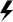
\includegraphics{graphics/logo_electricity}}
        \hbox{\hspace{9.8cm}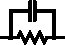
\includegraphics{graphics/logo_impedance}}
    }
  \end{center}
  \vspace{0.5cm}
  
  This thesis is separated into two parts, both linked to the behaviour of double-layers.
  In~\cref{part:doubleLayersOnInsulators} these layers are used as a means of converting fluid-mechanical energy into electrical energy.
  The primary application of such a harvester would be to power electronic water meters.
  Domestic water meters are typically installed where electrical connection is not feasible; harvesting energy here may makes electronic metering more feasible long-term.
  My findings show that double layer based energy harvesters are not efficient enough for this application yet.
  Recent literature on the subject suggests large gains in efficiency may be possible using more exotic materials.

  \Cref{part:doubleLayersOnConductors} models the electrical impedance of submerged electrodes.
  Double-layers play a large part in determining the electrical impedance between metal-fluid interfaces.
  This work is important to designers of medical implants; and by extension, anybody who relies on the implants themselves.
  Engineers use solutions of saline to mimic the environment experienced by their implants once implanted.
  This gives them a way to test the implant without injuring anyone.
  A way of characterising the interface between electrodes in solution is to model it mathematically.
  Such a model was created by my supervisor, Jonathan Scott.
  I use that model to compare electrodes placed in solutions of saline to those placed in a living animal.
  Measurements of the two show they are quite different from one another.
  I create a mixture using low-cost ingredients that closely resembles the electrical impedance of a live animal.

\phantomsection\addcontentsline{toc}{chapter}{Abstract}

\chapter*{Acknowledgement}
\phantomsection\addcontentsline{toc}{chapter}{Acknowledgement}
Thanks to Jonathan Scott (my chief supervisor), Steve Newcombe (Waikato University's award winning glass blower) and Peter Single (the senior electrical engineer at Saluda Medical) for their time, resources and patience.
Thank you to my second supervisor, Marcus Wilson, for checking up every so often and help proof-reading.
Thanks also go to the University of Waikato for a funding the first three years of this work with a Waikato Doctoral Scholarship.
Without this funding I could not have undertaken this research.
The support of my partner, Sarah, and my mother, Gina, has kept me on track.
Lastly, thank you to everyone who has contributed to open-source projects, especially those part of
\begin{itemize}
\item The Linux kernel and GNU tools
\item Gnome desktop environment
\item Inkscape vector drawing software
\item Gimp image manipulation program
\item The Arch Linux distribution
\item \TeX \space and its derivative \LaTeX
\item Python
\item ngSpice
\end{itemize}
Work done throughout this thesis has relied entirely on those tools

\tableofcontents{}
\listoffigures
\listoftables
\doublespacing

%% Introduction

\chapter{Introduction}
  \label{chap:introduction_main}
  \pagenumbering{arabic}
  %!TEX root = ../../thesis.tex


%% INTRODUCTION


Is it possible to harvest energy from water without moving parts?
What is the electrical impedance between electrodes in an electrolyte solution?
Although seemingly unrelated, the answer to both lies in behaviour that occurs where liquids comes into contact with solids.
That behaviour is the formation of arranged layers of liquid against the solid surface, called a double layer.
This thesis is separated into two parts, each addressing one of the two questions above related to double layers.
\Cref{part:doubleLayersOnInsulators} studies double layers on insulating solids as a means of energy conversion.
A number of double layer based power harvesters are fabricated and their output is measured.
Converting fluid energy into electrical using double layers would allow for a ``no moving parts'' or ``solid-state'' energy harvester.
Such a harvester could potentially outlast a mechanically based equivalents (due to reduced wear on moving components) and be cheaper to produce (owing to a lower component count).
One application of particular interest is smart metering of domestic water usage.
\Cref{part:doubleLayersOnConductors} models the electrical impedance between two electrodes when submerged in an electrolyte.
Double layers play a large role in this impedance as they dictate the concentration of ions at the electrode's surface.
Measurement of interface impedance allows for direct comparison between a range of environments into which electrodes are placed.
This is important when designing an implant that will be inserted into a person.
Before introducing background material on interfacial double layers, my motivation for doing this work is discussed.
This is followed by a statement of originality and an outline of the structure of this thesis.


\section{Motivation}
  \label{sect:introduction_motiviation}


  My research began with the question ``is it possible to harvest energy from water without moving parts?''
  The motivation to answer this question lay in the idea of building an energy harvester to power an electronic water meter.
  Doing this without the moving parts of more traditional mechanisms, such as turbines, should increase the harvester's life-span and be generally more robust.
  I started by looking at three possible harvesting mechanisms:
  \begin{itemize}
    \item piezoelectric oscillators,
    \item electrostatic generators, and
    \item streaming potential cells
  \end{itemize}
  The piezoelectric oscillator was the equivalent of a water whistle with a vibrational energy harvester attached.
  The electrostatic generator was a version of Lord Kelvin's Electrostatic Generator with a harvesting application~\cite{Thomson1867a}.
  And the streaming potential cell was a mystery at the time.
  We knew geologists used streaming potentials to measure underground water flow.
  The only thing we knew about the mechanism was that forcing water through something somehow generated a voltage.
  Learning about that mechanism and answering the following questions started me on the path that became this thesis.
  \begin{enumerate}
    \item Where does streaming voltage come from?
    \item What role does the geometry of a streaming device play?
    \item Could you change the materials to get more voltage?
  \end{enumerate}
  After experimentation and energy budgeting, I eventually concluded that streaming cell harvesters are not yet practical.
  Low conversion efficiency, a susceptibility to clogging and the need for high manufacturing tolerances make them unsuited for domestic water metering.
  However, this research allowed me to gain  a working knowledge of interfacial double layers.

  During my doctoral studies my supervisor, Jonathan Scott, took a sabbatical at Saluda Medical in Sydney.
  At the time, Saluda were developing a medical implant for spinal cord stimulation.
  Jonathan and Saluda's senior electronic engineer developed an electrical model of the impedance presented by electrodes immersed in a solution of saline.
  That model uses electrical components to simulate the electrical impedance between an electrode and an electrolyte.
  This means it can be entered into electrical simulation software and used to simulate an implanted electrode.
  Much of the behaviour the model simulates is due to double layers.
  Saluda's engineers use a dilute solution of phosphate buffered saline to approximate human spinal cavities into which their electrodes are implanted.
  They do not know how good this approximation is, but it was the most appropriate mixture they had.
  The alternative was to embed an electrode in a live animal and measure the response - that is also what they do.
  Live animal experiments are costly and how they differ from solutions of saline is still unknown.
  The interface model is the starting point for the second phase of my research, which characterises the interface between an electrode and biological solutions.
  I have leveraged my understanding of interfacial double layers from \cref{part:doubleLayersOnInsulators} to understand how the model worked, and use it correctly.


\section{Statement of Originality}

  The work contained in this thesis is my own except where otherwise acknowledged.
  % Measurements of the energy consumed during an EEPROM write, an ADC measurement, a single instruction being executed, and during sleep mode for six 8-bit microprocessors are my own.
  % The relationship between an electrolyte's conductivity and the impedance of the constant phase element, presented in~\Cref{part:doubleLayersOnConductors}, is my own.
  % The recipe for a mixture that improves the match between live sheep spine and saline is my own.
  % The measurement configuration for sampling Faradaic current which removes the effect of double layer capacitance between electrodes in an electrolyte is my own.


\section{Publications Arising From This Work}


  \begin{itemize}
    \item Jones, M.H. \& Scott, J. (2014). \emph{Scaling of Electrode-Electrolyte Interface Model Parameters In Phosphate Buffered Saline.} Published in IEEE Transactions on Biomedical Circuits and Systems, Issue 99.
    \item Jones, M.H. \& Scott, J. (2014). \emph{Feasibility of Harvesting Power to Run a Domestic Water Meter Using Streaming Cell Technology.} In proceedings of the 21st Electronics New Zealand Conference, ENZCON 2014, Waikato University, Hamilton, New Zealand.
    \item Jones, M.H. \& Scott, J.B. (2011). \emph{The energy efficiency of 8-bit low-power microcontrollers.} In Proceedings of the 18th Electronics New Zealand Conference, ENZCON 2011, Massey University, Palmerston North, 21-22 November 2011, pp. 87-90.
  \end{itemize}


\section{Thesis Outline}


  This thesis is broken into two parts.
  \Cref{part:doubleLayersOnInsulators} is concerned with energy harvesting with double layers, specifically by the use of streaming cells.
  \Cref{part:doubleLayersOnConductors} measures and models the impedance of an interface, specifically those between implant electrodes.
  Put simply, \cref{part:doubleLayersOnInsulators} deals with double layers on insulating surfaces, and \cref{part:doubleLayersOnConductors} deals with double layers on conductive surfaces.

  The next chapter (\cref{chap:background}) contains background material on double layers, including their formation and a breakdown of their structure.
  The topics of streaming cells and impedance modelling are introduced in that chapter.
  Then, \cref{part:doubleLayersOnInsulators} begins by looking at streaming cells for the purpose of running an energy harvesting water meter.
  It starts at \cref{chap:part1_streamingCellHarvesters} with a brief mathematical analysis, followed by streaming cell fabrication, and then measurements of their ability to harvest energy.
  \Cref{chap:part1_waterMetering} estimates the amount of energy that would be available to a streaming cell energy harvester.
  \Cref{chap:part1_energyHarvestingRequirements} looks at the amount of energy needed to run microprocessors and wireless transmitters.
  This concludes with an estimate of the amount of energy required to run an electronic water meter.
  To conclude \cref{part:doubleLayersOnInsulators}, \cref{chap:part1_conclusion} combines the data obtained and the feasibility of streaming cell energy harvesting for electronic water metering is discussed.

  The second part of the thesis (\cref{part:doubleLayersOnConductors}) starts with an overview of the electrode interface model (\cref{chap:theInterfaceModel}).
  \Cref{chap:interfaceParameters} deals with measurement of the various model parameters in both phosphate buffered saline (\cref{sect:pbs_measurements}) and inside a live sheep's spinal cavity (\cref{sect:sheep_measurements}).
  Finally, \cref{chap:fluid_mimicry} presents work on the creation of a mixture designed to better represent the environment inside sheep spine compared to phosphate buffered saline (PBS).


%% Part 1 - Energy Harvesting

\part{Double Layers on Insulators: Harvesting Energy}
  \label{part:doubleLayersOnInsulators}
  In~\cref{chap:introduction_main}, basic principles of double layers were put forward.
  It is the electrical conductivity of the solid material that divides the two topics of this thesis.
  \Cref{part:doubleLayersOnInsulators} looks specifically at double layer formation between liquids and non-conductive solids, e.g., glass.
  Later, in~\cref{part:doubleLayersOnConductors}, conductive materials will be examined with a rather different application.

  The previous introduction shows that double layers are simply collections of charged ions.
  Can we collect these ions and use them to generate electrical power?
  Doing so would provide a method of energy harvesting without moving parts.
  \Cref{part:doubleLayersOnInsulators} explores energy harvesting applications of interfacial double layers.
  I build and measure a streaming cell harvester at test the idea of using it to run an electronic water meter.
  To see if such an application is feasible, I create a power budget of energy available, and energy required by the electronics.
  This work is wrapped up with a discussion of practicalities and final conclusions regarding feasibility and future work.

  \chapter{Introduction}
    \label{chap:harvesterIntroduction}
    %!TEX root = ../../thesis.tex

{\color{red}
Background information specific to power harvesting and double layers on insulating surfaces}

  \chapter{The Streaming Cell Energy Harvester}
    \label{chap:harvestingEnergy}
    %!TEX root = ../../../thesis.tex

This chapter begins with a mathematical analysis of streaming cells and operating parameters.
Then, in \cref{sect:part1_energyHarvesting_buildingStreamingCells}, a variety of streaming cell designs are built.
Early attempts at making streaming cells are presented, followed by more successful streaming cell designs.
Ten streaming cells are made using that design with each having slightly different geometric dimensions.
The electrical output and energy conversion efficiency of these cells is measured in \cref{sect:part1_energyHarvesting_measuringStreamingCells}.
Measurement results are discussed in~\cref{sect:part1_energyHarvesting_discussion}, followed by my concluding remarks.


\section{General Analysis}
  \label{sect:part1_energyHarvesting_generalAnalysis}


  A basic model of operation for a streaming cell is established.
  This determines what parameters are important when maximising a cell's output power.


  \subsection{Mathematics}


    Mathematical analysis of streaming cells provides a basic understanding of the parameters involved with their output and geometry.
    Rigorous mathematical analysis of streaming cell performance is extremely involved and is well detailed in the literature~\cite{Yang1998}.
    As aspects of a double layer's structure are still not fully understood, the mathematics behind them is still being developed.
    Computer simulation and mathematical models continue to shed light on ionic organisation at liquid-solid interfaces~\cite{Kornyshev2007}.
    For that reason, I have not attempted to model a streaming cell physically.
    Instead, I piece together a relatively simple mathematical model quantifying important operating parameters.


    \subsubsection*{Streaming voltage}

      Gu and Li derived the following equation relating the streaming voltage to the pressure applied across a streaming cell~\cite{Gu2000}.
      \begin{equation}
      \frac{V_{s}}{\Delta P} = \frac{\varepsilon_{r}\,\varepsilon_{0}\,\zeta}{\mu(\sigma+\frac{2}{\delta}\lambda)}
      \label{eq:part1_energyHarvesting_streamingVoltage}
      \end{equation}
      \noindent where:
      \begin{description}
          \item $V_{s}$ is streaming voltage
          \item $\Delta P_{z}$ is pressure differential (across the channel)
          \item $\epsilon_{r}$ is the relative permittivity of the liquid
          \item $\epsilon_{0}$ is the absolute permittivity of free space
          \item $\zeta$ is zeta potential
          \item $\mu$ is the fluid's viscosity
          \item $\sigma$ is the fluid's bulk conductivity
          \item $\delta$ is the channel's height
          \item $\lambda$ is the channel's surface conductivity
      \end{description}
      This equation is specific to parallel plate channels, of the type constructed in the following section.
      It requires that the width to height ratio of the channel is greater than 20, which it is for the cells constructed here.
      Gu and Li use this equation as a means of finding the zeta potential and surface conductance by rearranging it into the following form:
      \begin{equation}
        \frac{\varepsilon_{r}\, \varepsilon_{0}\, \Delta P}{\mu\, V_{s}\, \sigma} = \frac{1}{\zeta} + \left(\frac{2\, \lambda}{\zeta\, \sigma}\right)\, \frac{1}{\delta}
      \end{equation}
      Later, the streaming voltage of ten cells with the same dimensions of those used by Gu and Li will be measured.
      The left hand side of this equation will be plotted against the inverse of channel height to see if their results can be replicated.
      If successful, this will give a way of determining the zeta potential and surface conductance of the fabricated cells.


    \subsubsection*{Streaming current}


      Gu and Li, also derive a similar equation for streaming current~\cite{Gu2000}.
      This equation, shown below, has been slightly rearranged to match the form of~\ref{eq:part1_energyHarvesting_streamingVoltage}
      \begin{equation}
          \frac{I_{s}}{\Delta P} = \frac{\varepsilon_{r}\,\varepsilon_{0}\,\zeta\,W\,\delta}{\mu\,L}
          \label{eq:part1_energyHarvesting_streamingCurrent}
      \end{equation}
      where
      \begin{description}
          \item $W$ is the width of the channel
          \item $L$ is the length of the channel
      \end{description}
      This equation is similar to that given by Olthuis et al.\ for a porous plug, but has been derived specifically for rectangular channels\cite{Olthuis2005}.


  \subsection{Electrical model}
    \label{sub:part1_energyHarvesting_generalAnalysis_electricalModel}


    % Model
    \begin{figure}
        \centering
            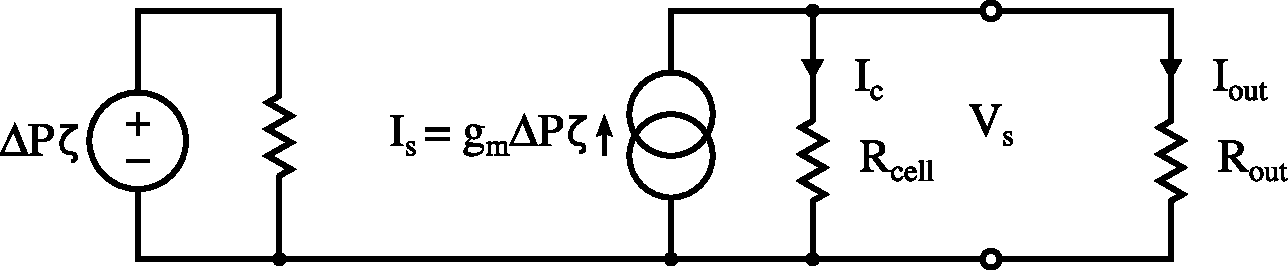
\includegraphics[width=\textwidth]{content/pt1/01-PowerHarvesting/graphics/StreamingCell_EquivalentCircuit_output}
        \caption{\label{fig:StreamingCell_Schematic-representation}Schematic diagram of a streaming cell with connected load resistance.}
    \end{figure}
    Figure \ref{fig:StreamingCell_Schematic-representation} depicts schematically how a streaming cell operates when connected to an external load.
    A model of this sort is commonly used to analyse the behaviour transistors.
    This particular model is based on the work of Olthuis et al.\ in \cite{Olthuis2005}, but has been modified slightly.
    Instead of showing $\zeta$ as the equivalent voltage source, it is shown here instead with the pressure applied ($\Delta P$).
    This change was made because there is no way of controlling the zeta potential - it determined by the properties of the particular interface.
    However, the amount of pressure developed across the cell is controllable, and from \cref{eq:part1_energyHarvesting_streamingCurrent} it is shown to be directly proportional to streaming current.
    In fact, the transconductance ($g_{m}$) for this model is \cref{eq:part1_energyHarvesting_streamingCurrent}.
    The model aids analysis in that it shows the electrical configuration of an external load resistance ($R_{out}$).
    As shown, any load resistance placed across the cell is being placed in parallel with the internal electrical resistance of the cell.
    This will help to determine how best to optimise the cell in order to maximise its electrical output.


  \subsection{Optimisation}

    Having a mathematical model of a streaming cell allows for optimisation of its operating parameters.
    The model shows that any load placed across a streaming cell is actually placed in parallel with that cell's internal resistance.
    Therefore, choosing a suitable load is an important design consideration.
    It is possible to optimise the cell's output for maximum power output, or maximum efficiency.
    So which is best suited to harvesting applications?

    Streaming cells are not batteries.
    The only time energy can be extracted from a streaming cell is when pressure developed across it.
    This only happens because of liquid flowing through it.
    When harvestable power is available, we need to collect as much of it as possible -- \emph{no matter how much is wasted}.
    Because a cell is incapable of storing energy, any energy that we could not capture will be lost.

    The story would be different for battery applications.
    In those situations would be advantageous to optimise for maximum efficiency.
    Doing so will conserve the energy in a battery and ensure that as little as possible goes to waste.
    This might be something a cell phone designer aims to achieve, but is less important for batteries accelerating an electric car.

    In situations requiring maximum efficiency, the efficiency of the system approaches \SI{100}{\percent} as the power delivered approaches \SI{0}{\percent}.
    In situations requiring maximum power, the maximum achievable efficiency is \SI{50}{\percent}.
    This means we can only harness half of the electrical power developed by a cell, at best.


    \subsubsection*{Optimising $R_{out}$ for maximum power}


      Using Ohm's Law it is possible to form an equation linking the total power ($P_{cell}$) to the total electrical resistance across the cell ($R_{tot}$).
      \begin{eqnarray}
          P & = & V\times I\nonumber \\
          V & = & I\times R\nonumber \\
          P & = & I^{2}\times R\nonumber \\
          P_{cell} & = & I_{s}^{2}\times R_{tot}
          \label{eq:DeterminingOutputPower_basic}
      \end{eqnarray}
      Where $I_{s}$ is the streaming current created by pumping ions through the channel.
      As the output resistance and internal cell resistance are in parallel we can find the output current ($I_{out}$) by treating the cell as a resistor divider (as is shown in~\cref{fig:StreamingCell_Schematic-representation}).
      Using a resistor divider equation for current in parallel branches yields:
      \begin{eqnarray}
          I_{out} & = & I_{s}\times\frac{R_{cell}}{R_{cell}+R_{out}}
          \label{eq:DeterminingOutputPower_extended}
      \end{eqnarray}
      Combining \eqref{eq:DeterminingOutputPower_basic} and \eqref{eq:DeterminingOutputPower_extended} we can extract the power dissipated in a load attached across the cell.
      \begin{eqnarray}
          I_{out} & = & I_{s}\times\frac{R_{cell}}{R_{cell}+R_{out}}\nonumber \\
          P_{out} & = & \left[I_{s}\times\frac{R_{cell}}{R_{cell}+R_{out}}\right]^{2}\times R_{out}
          \label{eq:DeterminingOutputPower_result}
      \end{eqnarray}

      Equation \eqref{eq:DeterminingOutputPower_result} takes into account the internal dissipation within the cell due to its own internal resistance.
      In order to optimise the output power it is necessary to find the value of output resistance ($R_{out}$) that maximises the output power.

      A parallel resistance system where we try to maximise the output power suggests this is a maximum power transfer theorem problem.
      The maximum power transfer theorem states that in order to maximise the power delivered to an external load from a source which itself has an internal resistance, one must make the two resistance equal.


    % \subsubsection*{Maximum power transfer theorem for a current source}


    %   This theorem is shown for resistors in series but no clear proof was found for a current source with two resistances in parallel.
    %   Here I prove that the maximum power theorem holds for a current source with resistors in parallel.
    %   This is not new work, but is included for completeness.

    %   First we take \cref{eq:DeterminingOutputPower_result} and treat the streaming current ($I_{s}$) as a constant, differentiate with respect to $R_{out}$ and find the condition that gives a maximum/minimum power output.
    %   \begin{eqnarray}
    %       P_{out} & = & \left[I_{s}\times\frac{R_{cell}}{R_{cell}+R_{out}}\right]^{2}\times R_{out}\nonumber\\
    %       \frac{P_{out}}{R_{out}} & = & \left[1\times\frac{R_{cell}}{R_{cell}+R_{out}}\right]^{2}\nonumber\\
    %       \frac{\partial P_{out}}{\partial R_{out}} & = & \frac{R_{cell}^{2}}{(R_{cell}+R_{out})^{2}}-\frac{2\times R_{cell}^{2}\times R_{out}}{(R_{cell}+R_{out})^{3}}\nonumber\\
    %       0 & = & \frac{R_{cell}^{2}}{(R_{cell}+R_{out})^{2}}-\frac{2\times R_{cell}^{2}\times R_{out}}{(R_{cell}+R_{out})^{3}}\nonumber\\
    %       \frac{2\times R_{cell}^{2}\times R_{out}}{(R_{cell}+R_{out})^{3}} & = & \frac{R_{cell}^{2}}{(R_{cell}+R_{out})^{2}}\nonumber\\
    %       \frac{2\times R_{cell}^{2}\times R_{out}}{R_{cell}+R_{out}} & = & R_{cell}^{2}\nonumber\\
    %       2\times R_{cell}^{2}\times R_{out} & = & R_{cell}^{2}\times(R_{cell}+R_{out})\nonumber\\
    %       2\times R_{out} & = & R_{cell}+R_{out}\nonumber\\
    %       R_{out} & = & R_{cell}
    %       \label{eq:maximumPowerTheorem_norton}
    %   \end{eqnarray}

    %   This shows that there is either maximum or minimum power transfer to $R_{out}$ when the value of $R_{out}$ matches that of $R_{cell}$.
    %   By plotting the power output as a function of the ratio of the two resistances (shown in \cref{fig:Plot-of-PowerTheorem}), we can see it is indeed a maximum.
    %   This shows the assumption of the maximum power transfer theorem in the case of streaming cell output to be correct.
    %   Usefully, it is shown that the absolute magnitudes of both $R_{out}$ and $R_{cell}$ have no effect on the output power - only their relative sizes (which in this case is equal).

    %   \begin{figure}
    %       \centering
    %           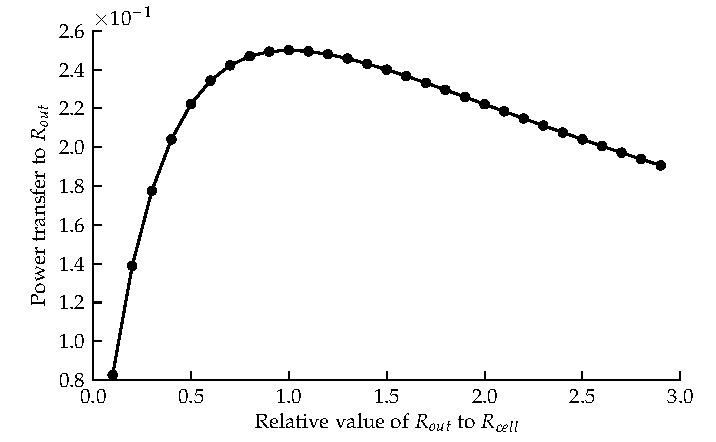
\includegraphics{content/pt1/01-PowerHarvesting/graphics/maximumPowerThereom}
    %       \caption{\label{fig:Plot-of-PowerTheorem}Plot of Equation \ref{eq:DeterminingOutputPower_result} when $I_{s}=1A$ and $R_{cell}=1\Omega$}
    %   \end{figure}


    \subsubsection*{Optimising streaming cell parameters}


      We now use the optimised values of $R_{out}$ and $R_{cell}$ to calculate the maximum available power.
      This is done by substituting $R_{out}$ and $R_{cell}$ for simply $R$ in \eqref{eq:DeterminingOutputPower_result} as follows.
      \begin{eqnarray}
          P_{out} & = & \left[I_{s}\times\frac{R_{cell}}{R_{cell}+R_{out}}\right]^{2}\times R_{out}\nonumber \\
          P_{max} & = & \left[I_{s}\times\frac{1}{2}\right]^{2}\times R\nonumber \\
          P_{max} & = & \frac{I_{s}^{2}R}{2}
          \label{eq:streamingCell_maxPower}
      \end{eqnarray}
      As $P=I^{2}R$ (via the power equation and Ohm's Law) this indicates at best we can capture half of the available power.

      It is now possible to combine the equation for maximum power, \eqref{eq:streamingCell_maxPower}, and that for streaming current, \eqref{eq:part1_energyHarvesting_streamingCurrent}.
      \begin{eqnarray}
          P_{max} & = & \frac{I_{s}^{2}R}{2}\nonumber \\
          P_{max} & = & \left(\frac{\varepsilon\,\zeta\,W\,\delta\,\Delta P}{\mu\,L}\right)^{2}\times\frac{R}{2}
          \label{eq:streamingCell_maxPower_substituted}
      \end{eqnarray}
      where $\varepsilon=\varepsilon_{0}\,\varepsilon_{r}$ and $R=R_{cell}=R_{out}$.

      To get a better feel for this equation, it may help to substitute in the parameters that affect $R$.
      From here we will refer to $R$ as the internal electrical resistance of the cell.
      It also refers to the external resistance in the maximum power condition, but we are free to vary that to match the internal resistance.

      We begin with the understanding that:
      \begin{eqnarray}
          R & \propto & \frac{L}{A\,\sigma}\label{eq:cell_resistance_electrical}\\
          R_{h} & \propto & \frac{L\,\mu}{A}\label{eq:cell_resistance_hydro}
      \end{eqnarray}
      where $\sigma$ is the conductivity of the liquid and $A$ is the cross-sectional area of the cell.
      The first equation \eqref{eq:cell_resistance_electrical} states that the electrical resistance will increase with cell length and decrease with the cross-sectional area of the cell and the conductivity of the fluid.
      The second \eqref{eq:cell_resistance_hydro} states that the fluid mechanical resistance will increase with the length of the cell and the viscosity of the fluid, and decrease with the cross-sectional area of the cell.

      We can identify the presence of $R_{h}$ in equation \eqref{eq:streamingCell_maxPower_substituted}.
      Starting with this equation we substitute equation \eqref{eq:cell_resistance_electrical} in and rearrange to produce an approximate relationship between pressure, cell length and area:
      \begin{eqnarray}
          P_{max} & = & \left(\frac{\varepsilon\,\zeta\,W\,\delta\,\Delta P}{\mu\,L}\right)^{2}\times\frac{R}{2}\nonumber\\
          P_{max} & \propto & \left(\frac{W\,\delta}{\mu\,L}\right)^{2}\times\left(\varepsilon\,\zeta\,\Delta P\right)^{2}\times \frac{L}{A\,\sigma} \times\frac{1}{2}\nonumber\\
          P_{max} & \propto & \left(\frac{A}{\mu\,L}\right)^{2}\times\left(\varepsilon\,\zeta\,\Delta P\right)^{2}\times \frac{L}{A\,\sigma} \times\frac{1}{2}\nonumber\\
          P_{max} & \propto & \frac{A^{2}}{L^{2}}\times\left(\frac{\varepsilon\,\zeta\,\Delta P}{\mu}\right)^{2}\times \frac{L}{A} \times\frac{1}{2\,\sigma}\nonumber\\
          P_{max} & \propto & \frac{A}{L}\times\left(\frac{\varepsilon\,\zeta\,\Delta P}{\mu}\right)^{2}\times\frac{1}{2\,\sigma}\nonumber\\
          P_{max} & \propto & \left(\frac{\varepsilon\,\zeta\,\Delta P}{\mu}\right)^{2}\times\frac{A}{2\,L\,\sigma}\nonumber\\
          P_{max} & \propto & \frac{\Delta P^{2}\,A}{L}\times \frac{\varepsilon^{2}\,\zeta^{2}}{2\,\mu^{2}\,\sigma}
          \label{eq:streamingCell_maxPower_relationship}
      \end{eqnarray}

      This equation \eqref{eq:streamingCell_maxPower_relationship} suggests that a cell with a small length, large area and high pressure is the best candidate for maximising power output.
      When using tap water we have no control over the remaining parameters; highlighting the importance of cell geometry and applied pressure.


\section{Streaming Cell Fabrication}
  \label{sect:part1_energyHarvesting_buildingStreamingCells}


  Building a streaming cell seemed a simple task at the outset.
  This section gives a brief overview of the work related to creating that first working streaming cell.


  \subsection{First streaming cells}


    \begin{figure}
      \centering
      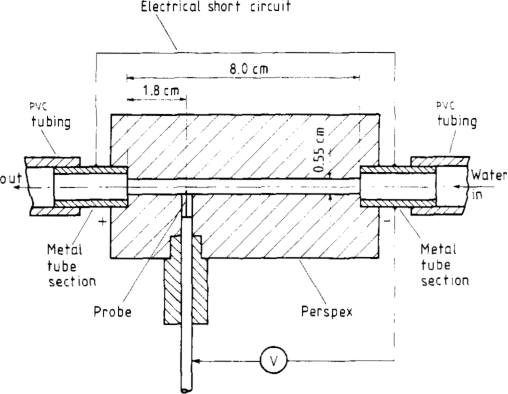
\includegraphics{content/pt1/01-PowerHarvesting/graphics/VargaSeymour1986_cell}
      \caption[Diagram of a cavitation device, taken from ~\cite{Varga1986}]{\label{fig:first_cell_diagram}Diagram of a cavitation device, taken from ~\cite{Varga1986}, reported to be able to generate over \SI{50}{\volt} across its ends by pumping water through it.}
    \end{figure}

    \begin{figure}
      \centering
      \includegraphics[scale=0.9]{content/pt1/01-PowerHarvesting/graphics/StreamingCell_v0}
      \caption[Photo showing a first generation of streaming device.]{\label{fig:first_cell}Photo of a first generation of streaming device. The device built by summer research student Jonathon McMullan to create the streaming voltages reported by Varga and Seymour.}
    \end{figure}
    \begin{figure}
      \centering
      \includegraphics[scale=0.7]{content/pt1/01-PowerHarvesting/graphics/StreamingCells_v1}
      \caption{\label{fig:first_cells}Photo showing two examples of a second design of streaming cell made entirely from glass.}
    \end{figure}

    The work that first sparked the interest of both my primary supervisor and I in streaming devices was that of Varga and Seymour~\cite{Varga1986}.
    In that paper it was reported that a device employing cavitation as a means of increasing the resistance between two bodies of  water was capable of developing over \SI{50}{\volt} across its ends.
    A diagram of the cavitation device is shown as \cref{fig:first_cell_diagram}.
    An attempt to replicate the results of that paper was made by summer research student Jonathon McMullan.
    Jonathon built a replica of the device, shown as \cref{fig:first_cell}; but was unable to reproduce streaming phenomena.

    My supervisor and I became sceptical of streaming cells at this point and looked elsewhere for energy harvesting ideas.
    The following year, summer research student Wane Crump and I conducted experiments to determine the amount of charge that could be transported on water droplets.
    This work was related to the idea of an electrostatic generator.
    See \cref{appendix:chargedDropletts} for details of the droplet based harvesting research.

    Later, other designs of streaming cells, namely those of Gu and Li~\cite{Gu2000}, were found in the literature.
    Their design of streaming cell looked simple and easy to fabricate, so attempts were made to replicate them.
    Employing Waikato University's glass-blower, Steve Newcombe, two streaming cells were fabricated entirely from soda-lime glass.
    These streaming cells are shown in \cref{fig:first_cells}.
    Each of the two channels were made by placing a \SI{50}{\micro\meter} sheet of copper between the glass slides; then wielding the glass slides together to seal the cell; and finally, etching the copper out with acid.
    The cells were then wielded (with glass) to the two side tubes that held the copper electrodes.
    By varying the length of the two channels (one of \SI{2}{\centi\meter}, the other \SI{4}{\centi\meter}) we hoped to determine what role length played on channel output characteristics.

    Both of the cells burst under the water pressure applied from lab taps.
    A crack along the right hand reservoir is visible on the \SI{2}{\centi\meter} wide channel.
    Attempts were made to strengthen the channels by coating joins with industrial glues, but none were successful.


  \subsection{Robust streaming cells}


    The two previous attempts to create streaming cells had failed.
    In the moments before failure, the all-glass streaming cells developed measurable voltage across their terminals.
    I knew I was close, but the all-glass design needed revising to increase the amount of pressure they could hold.
    A new design was found that solved the problem of cracking.
    It favoured the used of epoxy resin and acrylic to contain the channels, allowing for more flex without the risk of cracking.
    Aspects of the design were taken from a paper by Gu and Li~\cite{Gu2000}.

    \begin{figure}[p]
      \centering
      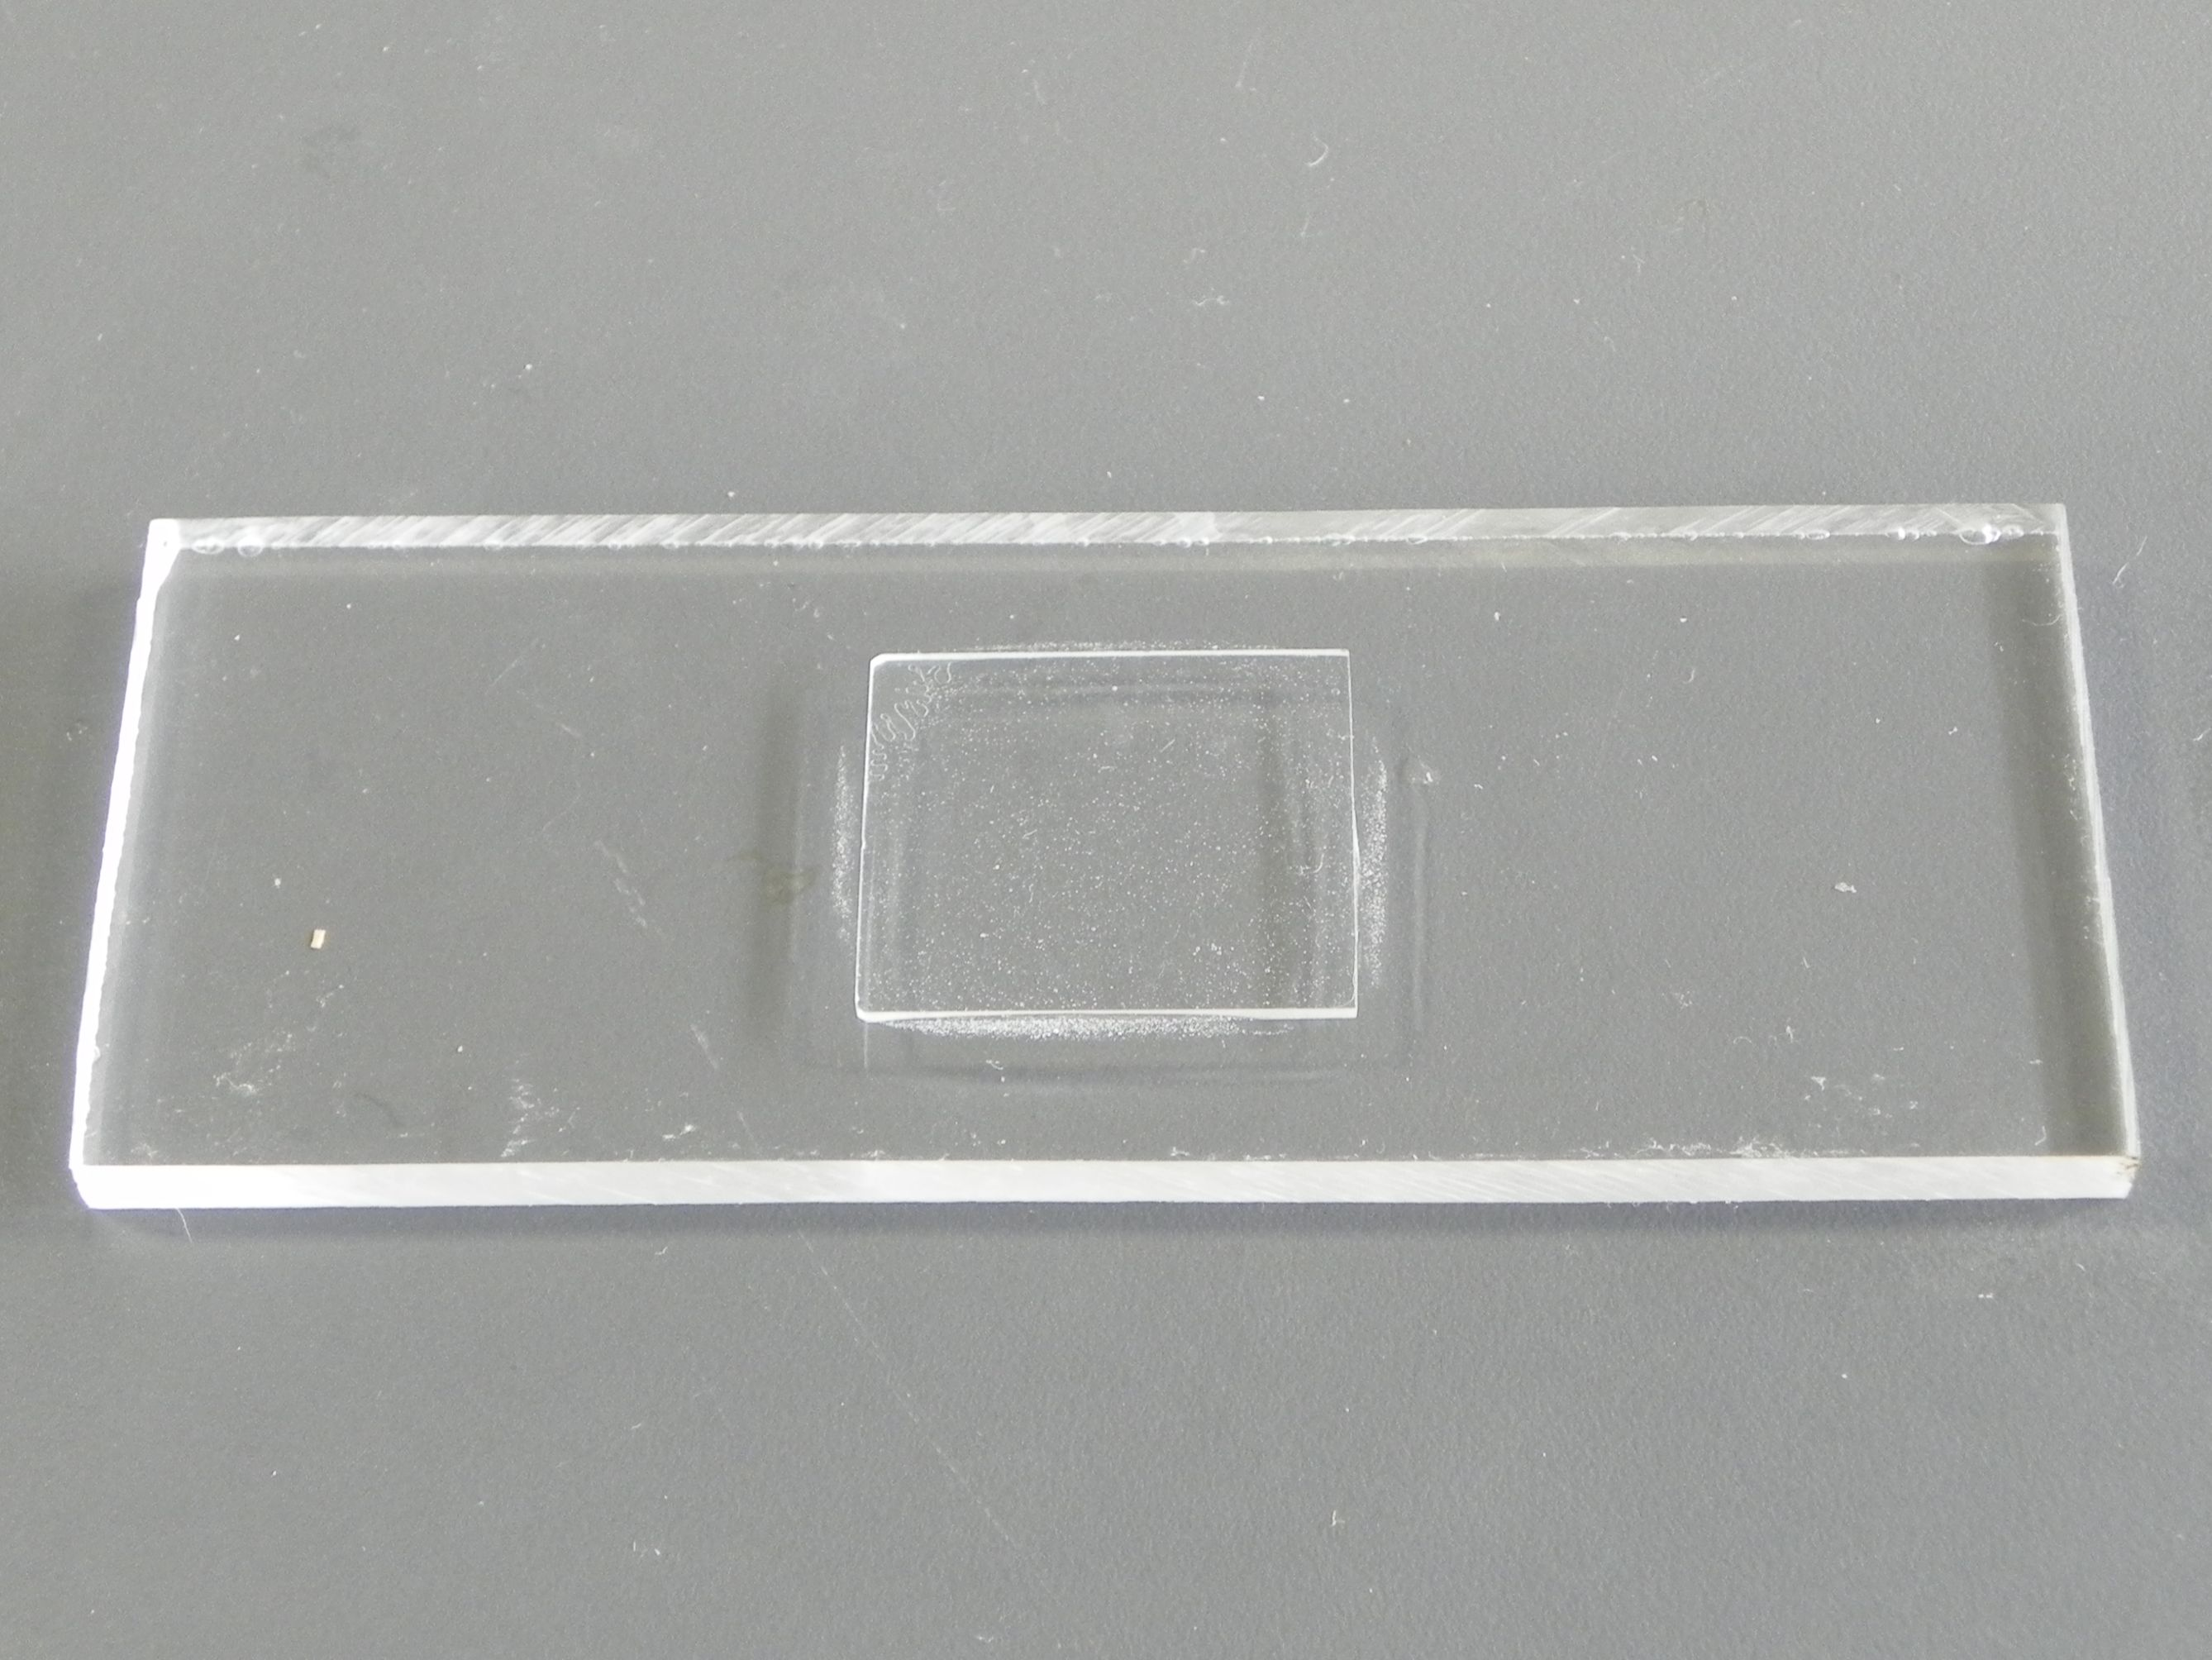
\includegraphics[width=0.5\textwidth]{content/pt1/01-PowerHarvesting/graphics/Photo_streamingPotential_Assembly_Step1.JPG}
      \caption{\label{fig:Photo_streamingPotential_Assembly_Step1}Photo showing half of a glass slide glued to acrylic base plate. Part of the process for constructing a streaming cell.}
    \end{figure}
    \begin{figure}[p]
      \centering
      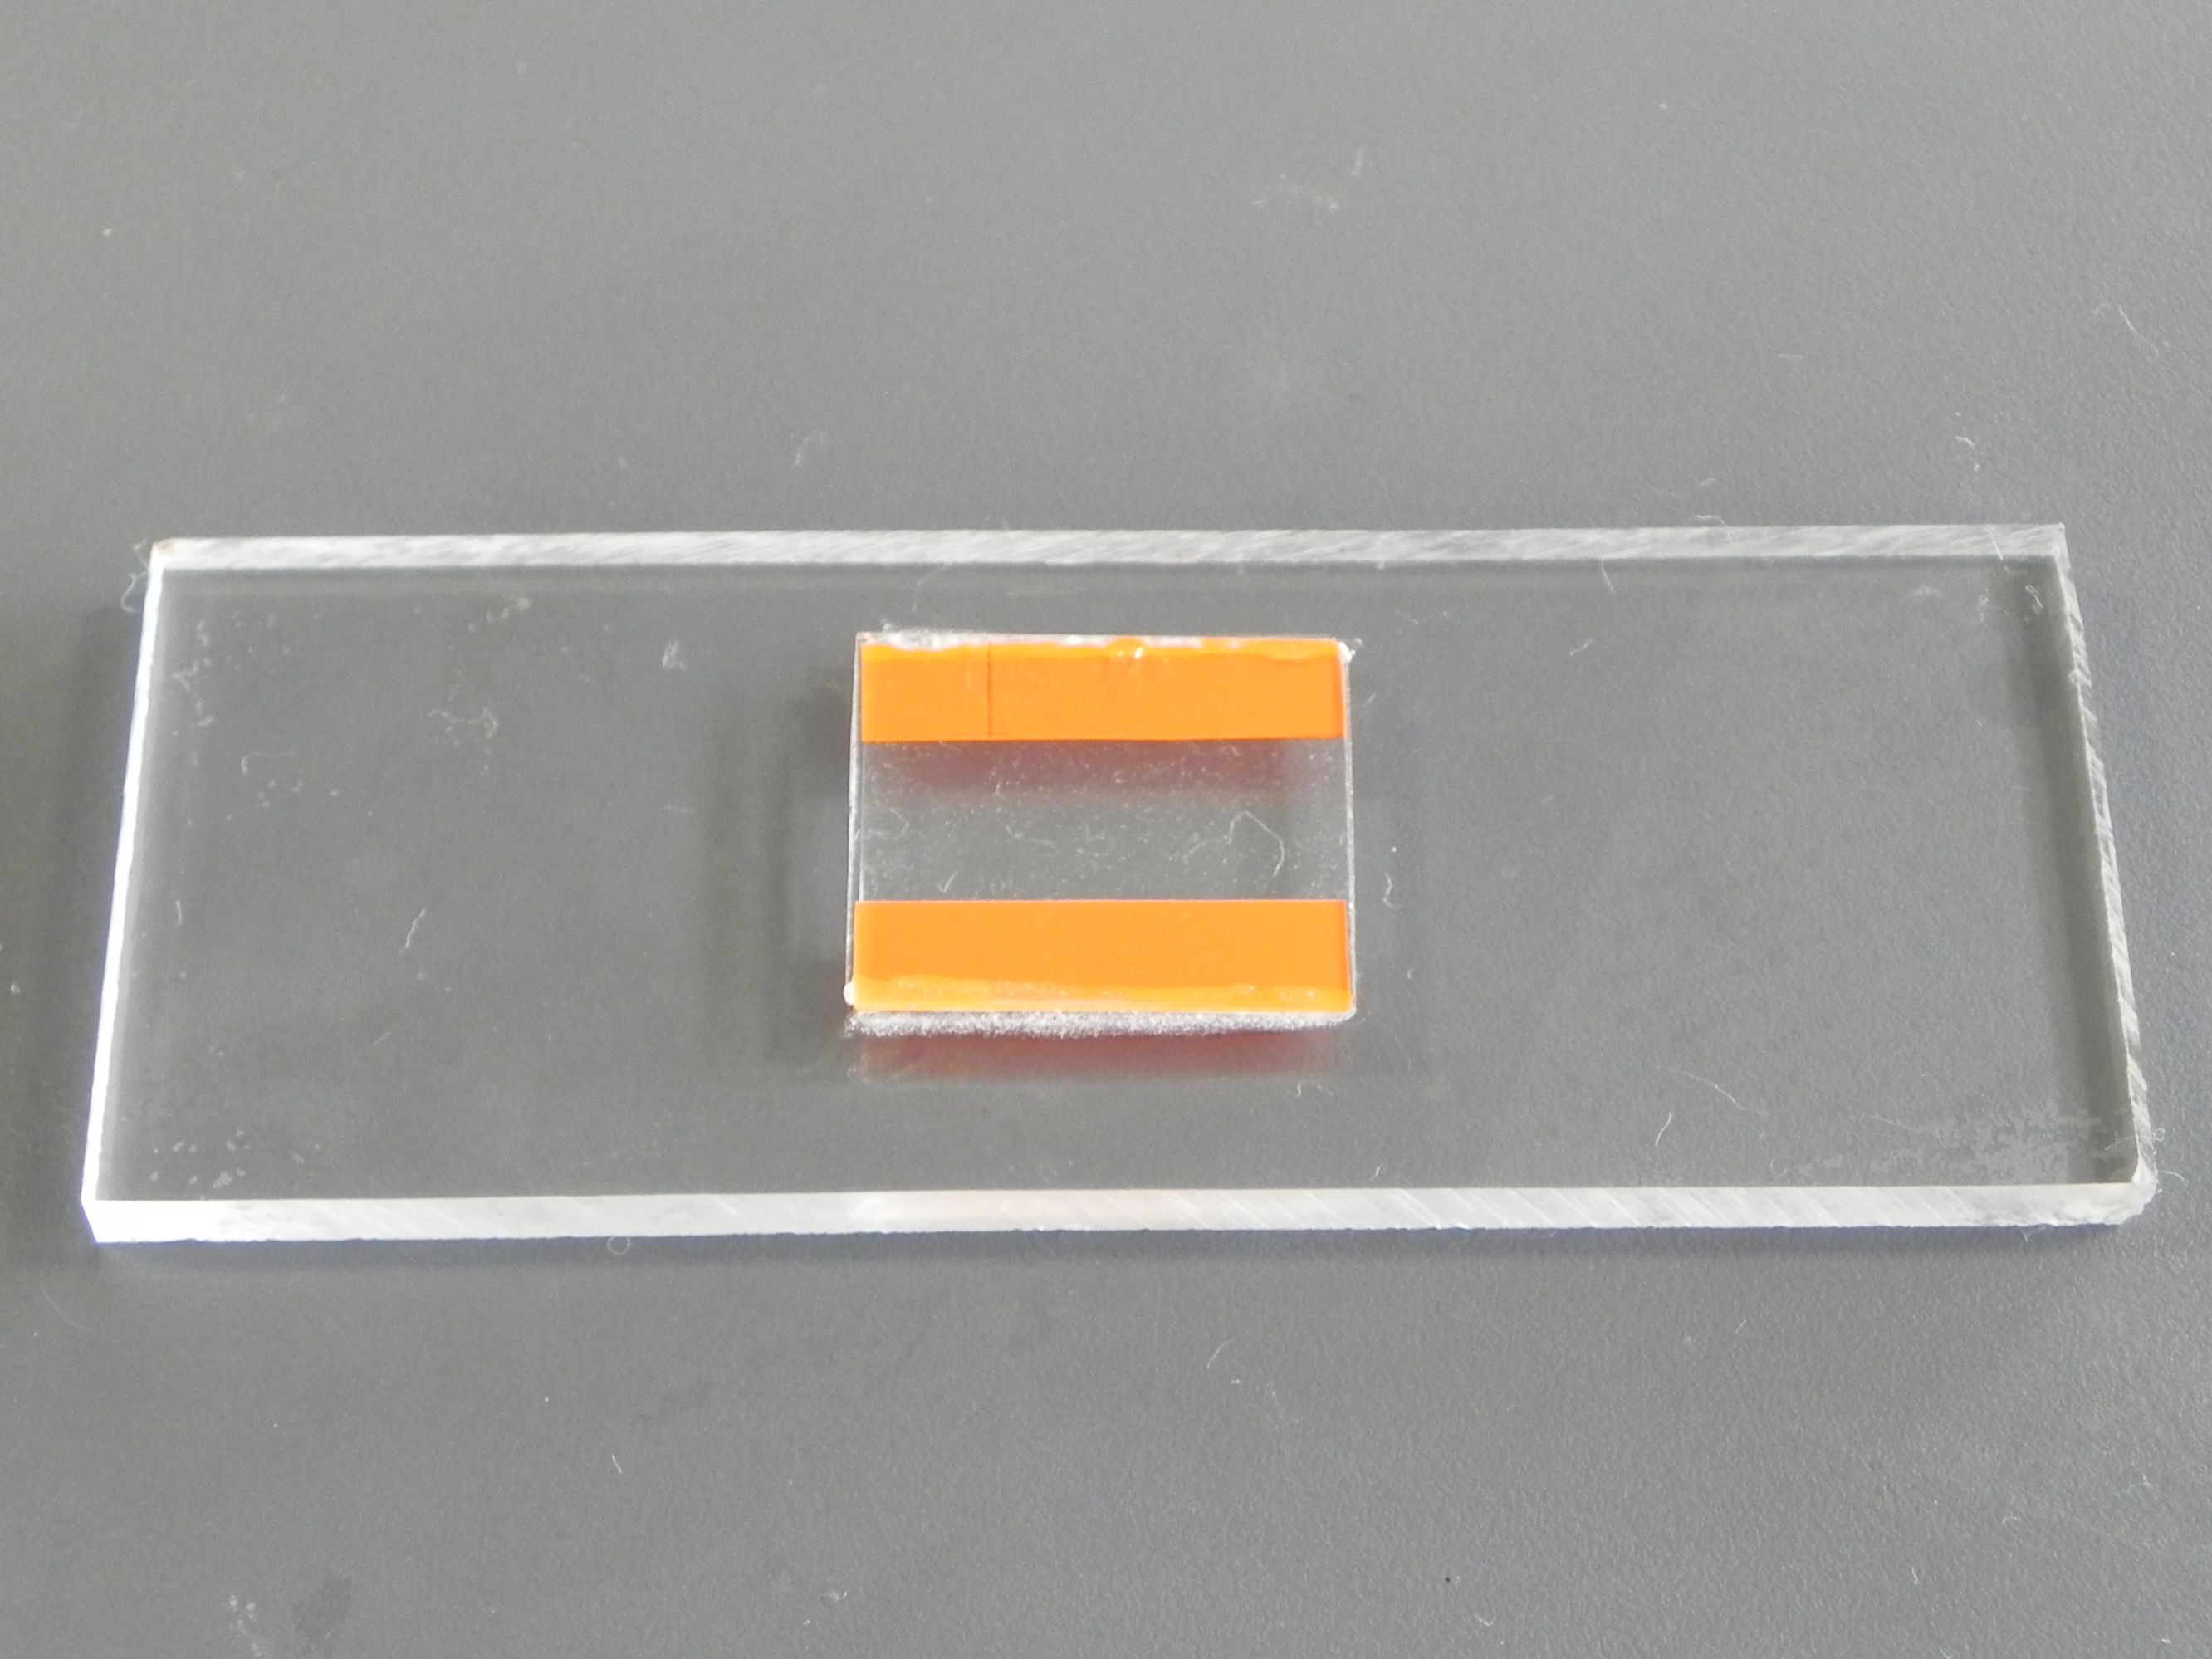
\includegraphics[width=0.5\textwidth]{content/pt1/01-PowerHarvesting/graphics/Photo_streamingPotential_Assembly_Step2.JPG}
      \caption{\label{fig:Photo_streamingPotential_Assembly_Step2}Photo showing plastic shims sandwiched between two slide halves. Part of the process for constructing a streaming cell.}
    \end{figure}
    \begin{figure}[p]
      \centering
      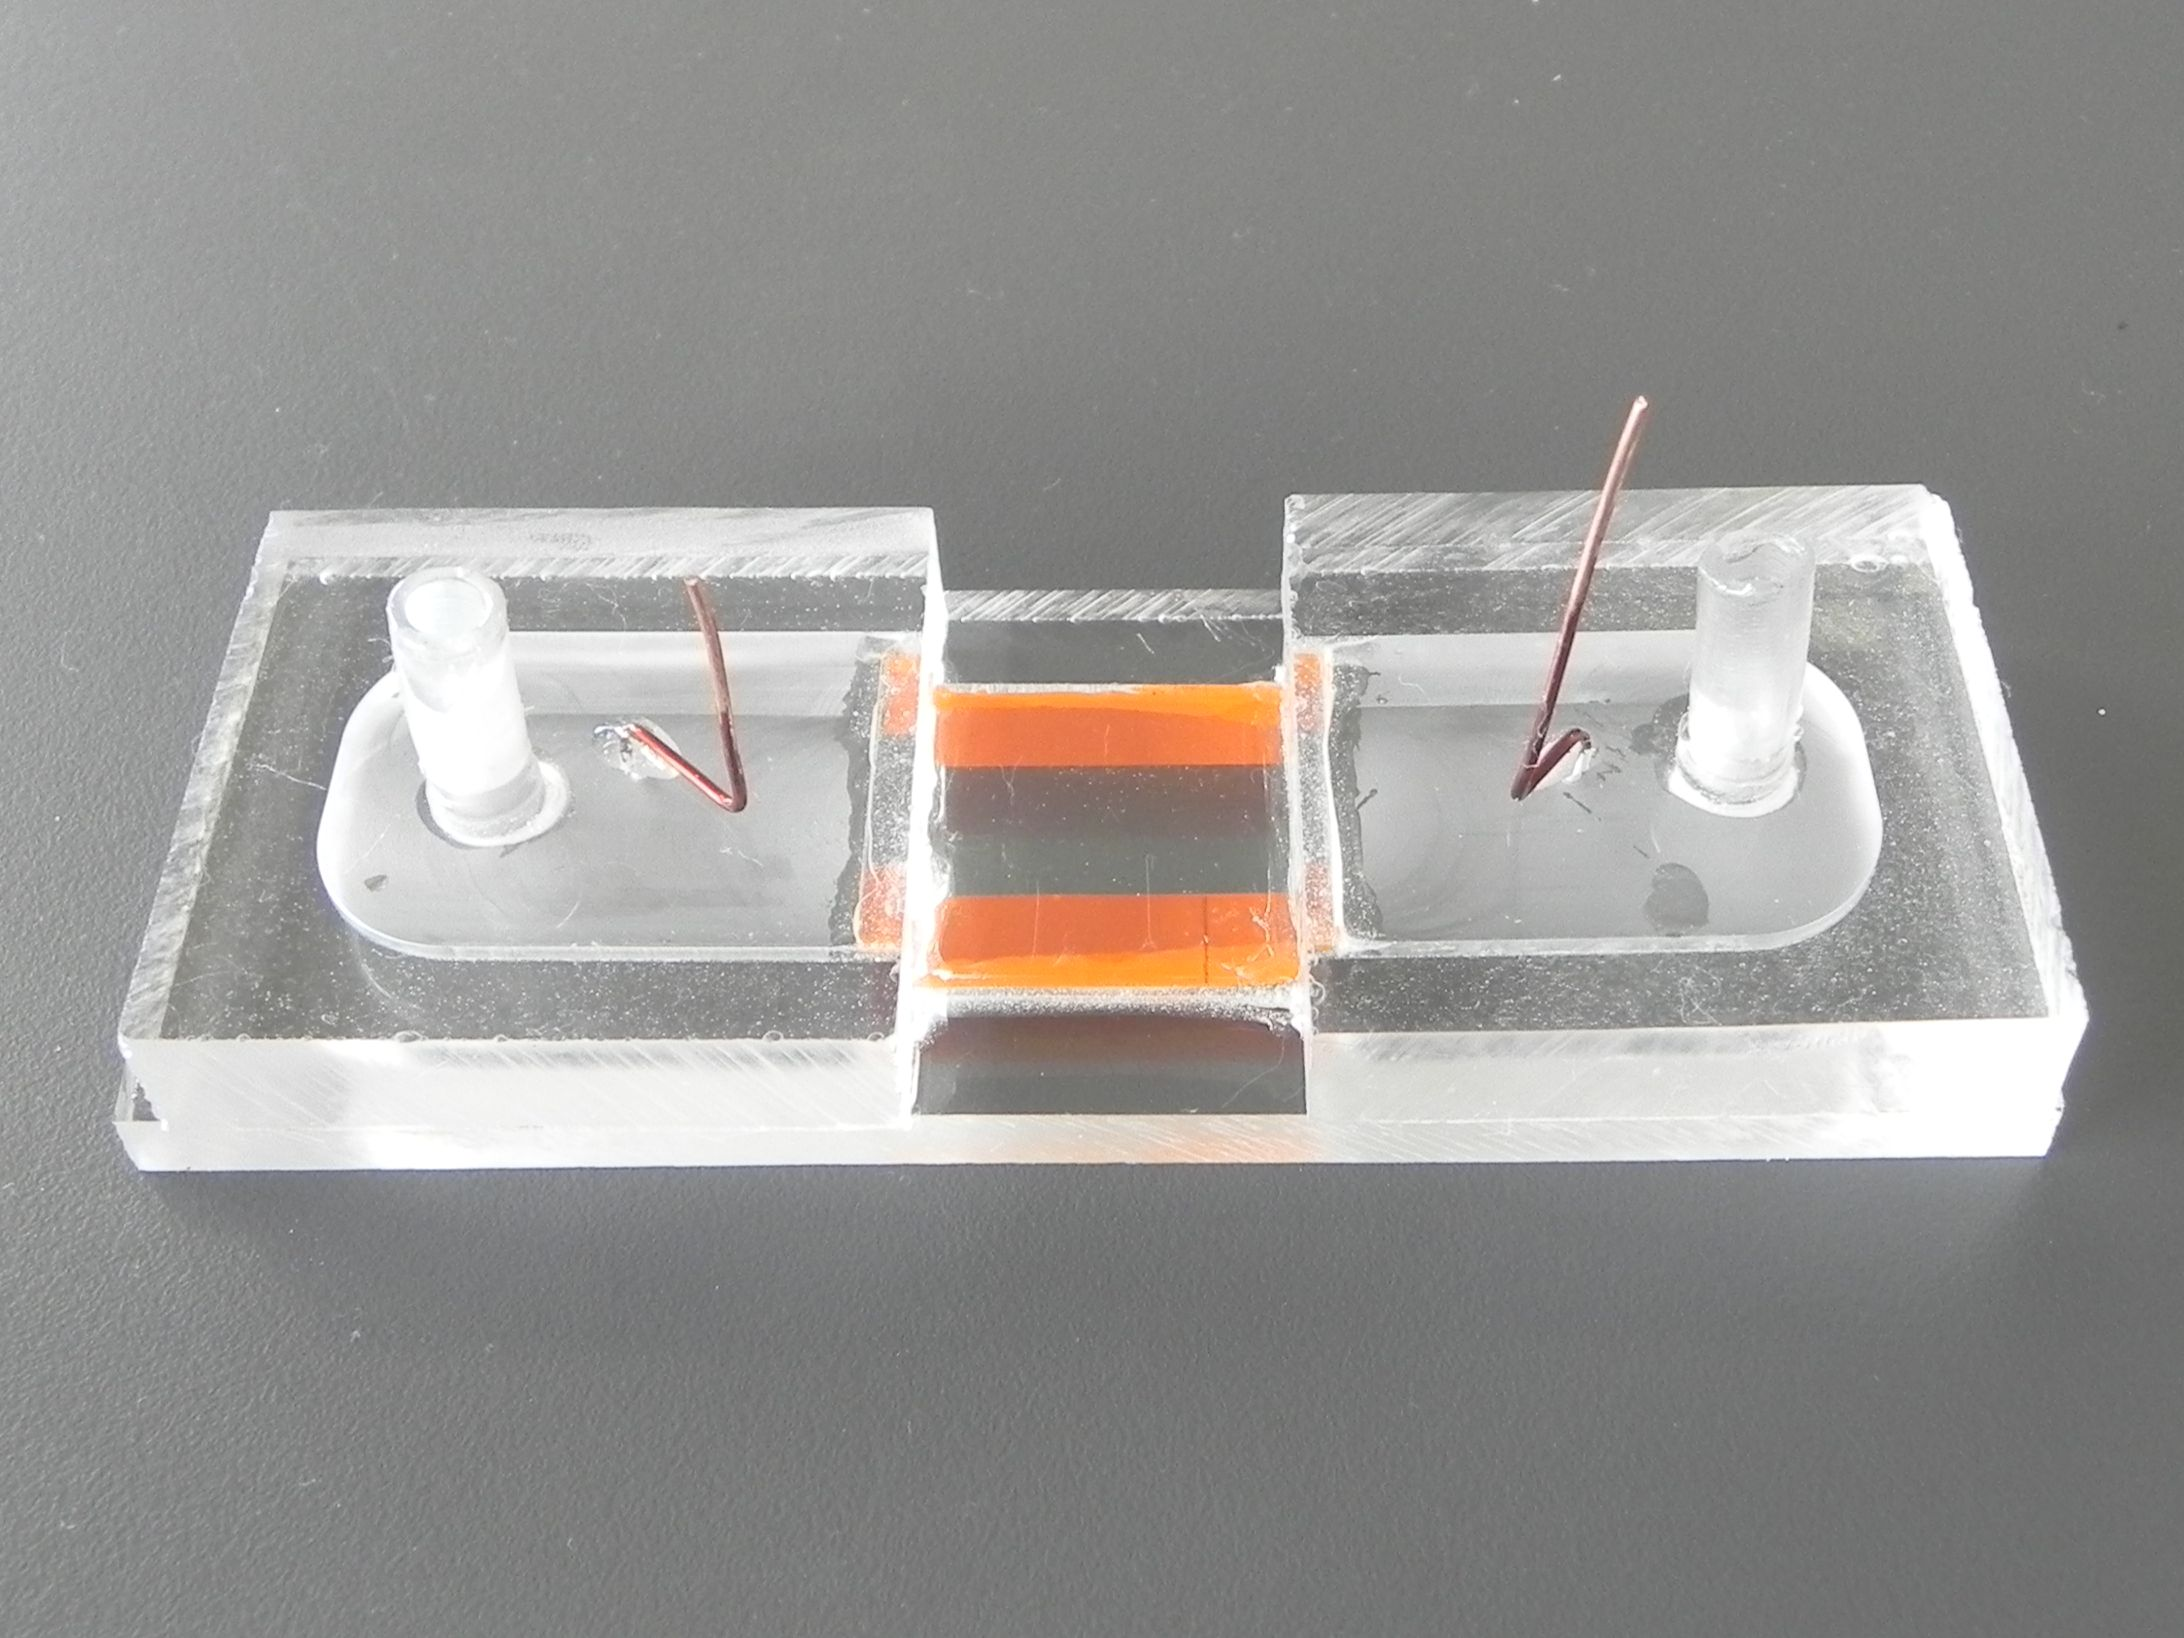
\includegraphics[width=0.5\textwidth]{content/pt1/01-PowerHarvesting/graphics/Photo_streamingPotential_Assembly_Step3.JPG}
      \caption{\label{fig:Photo_streamingPotential_Assembly_Step3}Photo showing final streaming cell assembly.}
    \end{figure}


    \subsubsection*{Construction}

      \begin{table}
        \begin{tabular}{r|c|l}
          Item & Brand & Product details\tabularnewline\hline
          Microscope slides & Sail Brand & JIA 7101WT - 26 x 76mm\tabularnewline
          Shims & Garlock & Colorplast - 50$\,\mu$m,80$\,\mu$m, 120$\,\mu$m and 250$\,\mu$m\tabularnewline
          Epoxy & Selleys & Araldite - Ultra Clear Resin\tabularnewline
          Pressure sensor & Honeywell & 24PC15SMT - 0 -- $\pm$15 PSI\tabularnewline
        \end{tabular}
        \caption{\label{Table_StreamingCell_MaterialsUsed}Materials used to construct the streaming potential cells}
      \end{table}
      Construction begins by sectioning standard microscope slides into halves.
      This gives glass panels of approximately \SI{26}{\milli\meter} $\times$ \SI{38}{\milli\meter} $\times$ \SI{1}{\milli\meter}.
      A single panel is then epoxied to an acrylic base plate, as is shown in Figure~\ref{fig:Photo_streamingPotential_Assembly_Step1}.
      Once set, plastic shims are cut to the required size, covered with a very thin layer of epoxy, and placed along the edges of the slide.
      The shims line the sides of the glass panel such that they leave a \SI{1}{\centi\meter} gap through the centre.
      A second glass slide is then placed on top of the shims and epoxy resin is used to seal the sides.
      Pressure was applied to the stack while the epoxy set to ensure the epoxy was distributed correctly and to control the channel height.
      A photo of the shims glued between the two slide halves is shown in Figure~\ref{fig:Photo_streamingPotential_Assembly_Step2}.
      Once set, each channel is examined under a microscope to determine the internal channel height.
      Each of the four corners were measured to ensure the internal dimensions remained rectangular once set.
      To finish, acrylic reservoirs where mounted over each end of the channel.
      These reservoirs facilitate the connection of fluid tubes and voltage probes to each end of the channel.
      The final assembly is shown in Figure \ref{fig:Photo_streamingPotential_Assembly_Step3}.
      A full list of materials used to construct the channels is presented as Table~\ref{Table_StreamingCell_MaterialsUsed}.
      A total of ten channels were made and tested using this method.


\section{Measurements}
  \label{sect:part1_energyHarvesting_measuringStreamingCells}


  Of the papers describing experiments using streaming potential cells (\cite{Gu2000,Mala1997,Scales1992,VanderHeyden2006}), I chose that of Gu and Li to replicate~\cite{Gu2000}.
  Their method employs a simple cell design, discussed in the previous section, and a detailed description of the experimental procedure.
  This section details measurement of ten streaming cells based on those of Gu and Li.


  \subsection{Experimental setup}
    \label{sub:part1_energyHarvesting_measuringStreamingCells_experimentalSetup}


    Measurement of each harvester was made in a laboratory using high-sensitivity measurement instruments and a lab water tap.
    Each cell's output power was measured with a precision source measurement unit (SMU) and applied pressure was monitored with a differential pressure sensor.

    The Agilent E5270B is a mainframe system that holds banks of SMUs with connections to a GPIB computer interface.
    The Department of Engineering's E5270 contains three SMUs, each having the ability to measure currents as low as one femto-Ampere.
    The device uses separate `force' and `sense' connections to ensure the voltage/current being set is accurately controlled where they meet.
    Additionally, it uses tri-axial cables to minimise any interference from outside sources; important when measuring such low currents.

    The input resistance to the E5270's measurement units are specified as \SI{13}{\giga\ohm}.
    It is essential to use such a high impedance measurement due to the high internal resistance of the cell.
    I later show that the internal electrical resistance of the cell is in the order of \SI{5}{\mega\ohm}, so the E5270's input impedance is roughly two thousand times larger.
    The internal resistance of a typical multimeter is \SI{10}{\mega\ohm}, too close to that of the cell and would therefore affect the measured output.

    The pressure sensor used was a Honeywell 26PC SMT Series differential pressure sensor.
    It comes as surface mount package, making it a cost effective solution, but delicate to set up.
    On its exterior are two ports to which rubber tubes are attached.
    Between those ports, internal to the sensor, sits a diaphragm.
    That diaphragm controls the resistance between two nodes in the sensor's bridge circuit (shown in figure \ref{fig:PressureSensorSchematic}).
    \begin{figure}
        \centering
        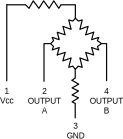
\includegraphics{content/pt1/01-PowerHarvesting/graphics/PressureSensorSchematic}
        \caption{\label{fig:PressureSensorSchematic}Schematic diagram of the differential pressure sensor bridge circuit (taken from \cite{Honeywell2003})}
    \end{figure}
    By applying \SI{10}{\volt} DC between the `Vcc' and `GND' pins, the output voltage between outputs `A' and `B' correspond to the applied pressure.
    Measurement of that output voltage was done using the precision measurement mainframe.

    The mainframe was controlled from a PC running Python scripts utilising the open source Python-vxi11 library~\cite{Python-ivi2014}.
    This allows sweeping the amount of current drawn from the harvester while recording the corresponding voltage drop.
    This is the equivalent of varying the load resistance, which allows us to find the point of maximum power transfer.

    \Cref{fig:measurementSetup} shows the measurement setup as a diagram.
    It shows connection of the measurement mainframe, bench-top power supply, streaming cell, pressure sensor, and the lab tap.
    Table~\ref{tab:measurementSetup_legend} provides details of the abbreviated electrical connection labels used in the figure~\ref{fig:measurementSetup}.

    \begin{figure}
        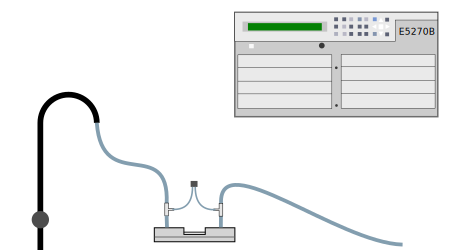
\includegraphics{content/pt1/01-PowerHarvesting/graphics/measurementSetup}
        \caption{\label{fig:measurementSetup}Diagram showing the measurement setup used to measure power output from streaming cell energy harvesters.}
    \end{figure}

    \begin{table}
        \centering
        \begin{tabular}{r|l}
        CELL - A & Voltage/current at high-pressure side of cell\\
        PRESS. - A & Output A of pressure sensor\\
        PRESS. - B & Output B of pressure sensor\\
        CELL - B & Voltage/current at low-pressure side of cell
        \end{tabular}
        \caption{\label{tab:measurementSetup_legend}Definitions for labels used in \cref{fig:measurementSetup}}
    \end{table}


  \subsection{Measurement issues}


    There are two issues with the measurement setup that may impact the measurements.
    Firstly, the electrodes used were copper and are susceptible to polarisation by electrolysis.
    Secondly, the differential pressure sensor is only rated to 15\thinspace PSI (approximately \SI{100}{\kilo\pascal}), less than half the maximum pressure developed across the cell.

    Electrolysis on at the electrode surface causes the electrodes to polarise.
    This results in a semi-permanent offset voltage appearing between the electrodes.
    That offset voltage is opposite in polarity to what is developed while cell is in operation.
    By reversing the flow of water through the cell the polarisation can be reversed.
    Use of more suitable electrode materials would reduce this effect, for instance platinum black electrodes.
    Copper was used for the electrodes as it was cheap, easily obtainable, and easy to work with.
    Offset voltages can be removed after measurement by subtraction.
    Obviously this is not a perfect solution but will be sufficient as the offset itself can be measured so it will be well known.

    From measurement of the output \emph{voltage} of the cells, the presented graphs and figures have been adjusted to remove the effects of electrolysis.
    This was done by adding an offset to the measured data to shift the y-intercept up to \SI{0}{\volt}.
    This provides a more accurate representation of the situation had platinum black electrodes been used.
    As no absolute data is taken from these measurements, the y-intercept adjustment does not affect any subsequent predictions made about the cells.
    Only the gradient of the output, relative to the pressure applied is used; and even then, only to select a suitable candidate cell for power measurement.
    \emph{Most importantly}, no offsets have been applied to measurements of the cell power output.

    Although the maximum rated pressure of sensor was 15\thinspace PSI (approximately \SI{100}{\kilo\pascal}), the sensor's output remained linear up to our maximum pressure of 40\thinspace PSI (\SI{275}{\kilo\pascal}).
    I expect that exceeding the sensors specified pressure will result in a lower `mean time to failure', but its output remained true.
    As a precaution, a tyre pressure gauge was used to roughly confirm the output of the sensor at the end of the cell measurements.
    This was a crude test, however it's output matched that of the differential pressure sensor, so was taken as a good indication of its accuracy.


\section{Results}
  \label{sect:part1_energyHarvesting_results}


  Results from streaming cell measurement are broken into two sub-sections.
  The first presents the output voltage of the ten cells in response to applied water pressure.
  From these measurements, the cell with the highest voltage/pressure ratio is found.
  The second sub-section shows the maximum power that can be harvested from that cell.
  These are the most important measurements as they reveal the energy conversion efficiency of the cells.


  \subsection{Streaming voltage versus pressure}



    \Cref{fig:streamingCell_all_adjusted} shows adjusted results of streaming voltage measurements from each of the ten cells.
    A full set of figures, one cell per graph, can be found in \cref{appendix:streamingCellMeasurements} as \Crefrange{fig:VvsP_26um}{fig:VvsP_245um}.
    It represents the first successful measurements I had made of streaming cells.
    During these measurements three cells burst under pressure; two were dropped and subsequently shattered; and one suffered epoxy failure, loosing its acrylic base plate.
    No measurements of flow rate or output current were made during these early experiments.
    As a result they reveal very little about the efficiency of the cells themselves.
    We cannot determine either the mechanical energy put into the cells, nor the output power available.
    However, we can relate these measurements to those made by Gu and Li; as will be shown and discussed shortly.

    \begin{figure}
        \centering
        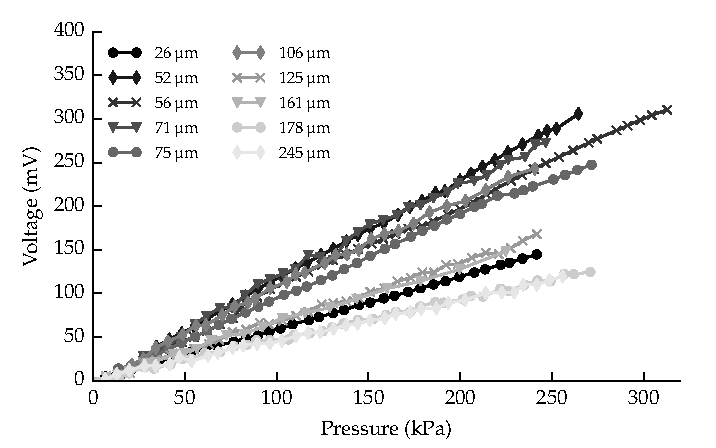
\includegraphics{content/pt1/01-PowerHarvesting/graphics/graph_streamingVoltageGradient_vs_height}
        \caption{\label{fig:streamingCell_all_adjusted}Plot showing adjusted streaming voltages versus applied pressure.}
    \end{figure}

    \begin{figure}
        \centering
        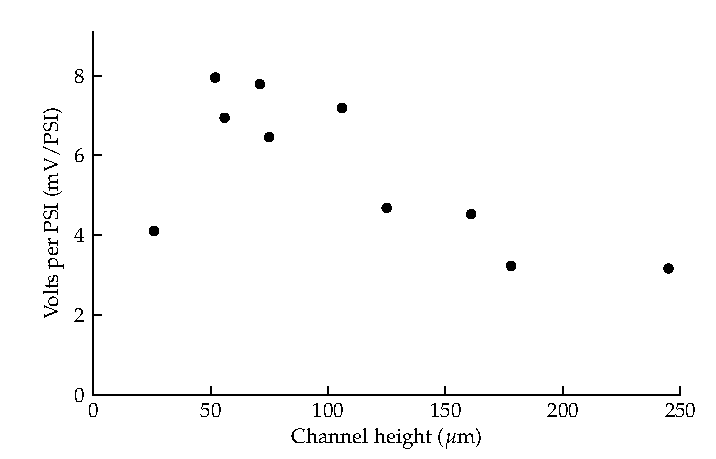
\includegraphics{content/pt1/01-PowerHarvesting/graphics/streamingCell_slopeVsChannelHeight}
        \caption{\label{fig:streamingCell_scatter_voltGradVsHeight}Scatter plot of voltage/pressure gradient versus channel height for each of the measured channels.}
    \end{figure}

    \begin{figure}
        \centering
        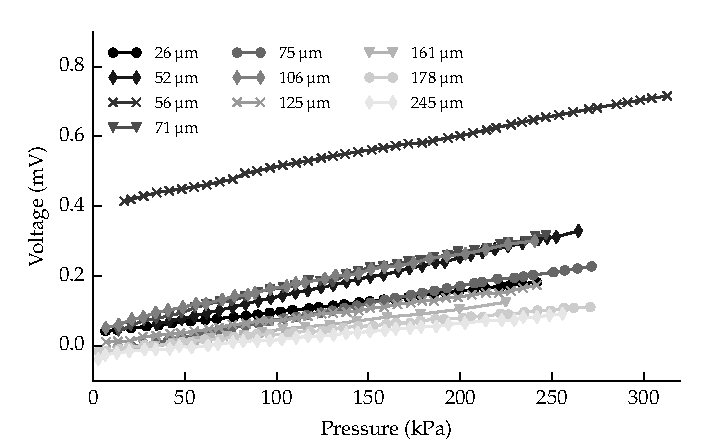
\includegraphics{content/pt1/01-PowerHarvesting/graphics/graph_streamingVoltageGradient_vs_height_noCorrection}
        \caption{\label{fig:streamingCell_all_unadjusted}Plot showing unadjusted streaming voltages versus applied pressure.}
    \end{figure}

    The cell having an internal height of \SI{56}{\micro\meter} required an offset adjustment of \SI{405}{\milli\volt} to remove its vertical offset.
    This indicates that the electrodes were highly polarised by the time measurements were made.
    This effect is especially evident in \cref{fig:streamingCell_all_unadjusted}, which shows raw measured data without vertical offset adjustment.
    Some of the traces exhibit a certain amount of `jitter' in their pressure-to-voltage gradients.
    This is likely due to the time difference between adjacent measurement points.
    Measurement points were not taken monotonically, instead being extracted from a number of pressure cycles.

    \Cref{fig:streamingCell_scatter_voltGradVsHeight} shows the streaming voltage to pressure gradients versus channel height.
    This data has been taken from the previous graph (\cref{fig:streamingCell_all_adjusted})) to show the response as a function of channel height.

    % Edit checkpoint 2015-09-13 19:43


  \subsection{Output power versus load resistance}


    \begin{figure}
        \centering
        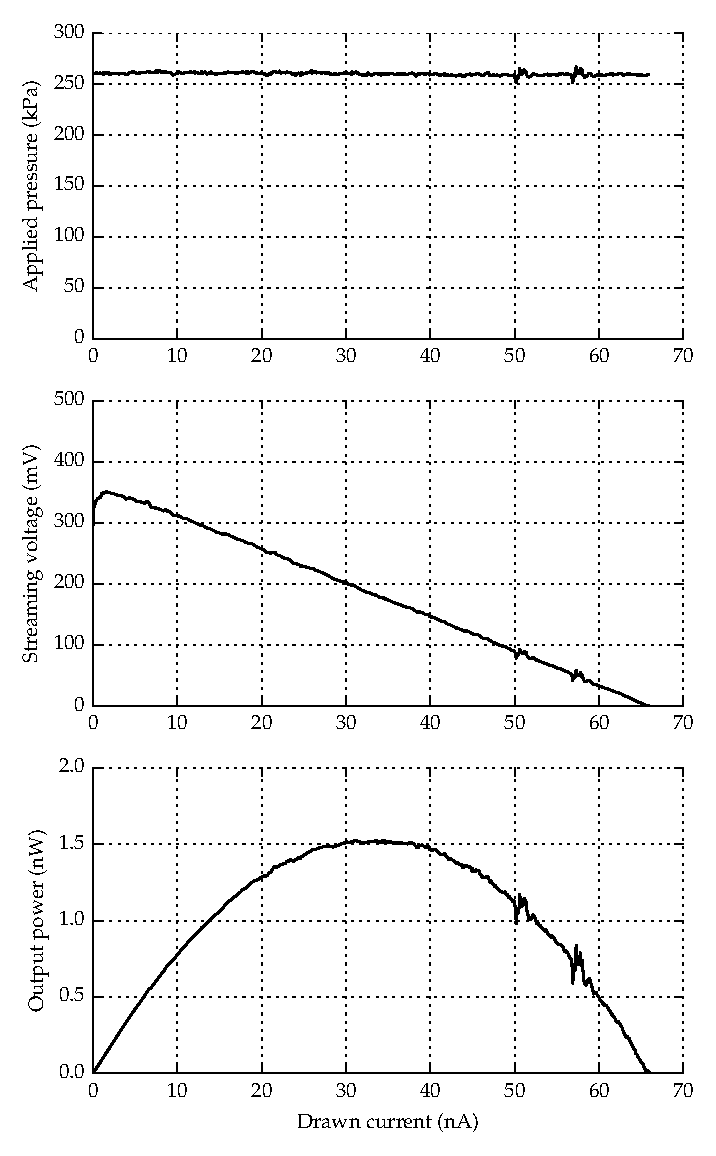
\includegraphics{content/pt1/01-PowerHarvesting/graphics/graph_streamingCell_outputPower_resistanceSweep}
        \caption{\label{fig:streamingCell_maxPower}Graph showing output power versus effective load resistance for a \SI{71}{\micro\metre} high channel at a pressure of \SI{260}{\kilo\pascal}.}
    \end{figure}

    \Cref{fig:streamingCell_maxPower} shows the characteristic power curve of the \SI{71}{\micro\meter} high streaming cell channel.
    Pressure fluctuations near the end of the experiment are due to usage of the departments water system.
    Their effect is visible in both the streaming voltage and output power traces, highlighting the strong coupling to applied pressure.

    The maximum power delivered by the cell was \SI{1.52}{\nano\watt}, corresponding to a current draw of \SI{33.5}{\nano\ampere} with a streaming voltage of \SI{182}{\milli\volt}.
    Generating this power required \SI{260}{\kilo\pascal} of pressure, resulting in a flow rate of \SI{2.05}{\milli\litre\per\second}.
    This equates to \SI{539}{\milli\watt} of pumping power lost to the device and therefore an energy conversion efficiency of \SI{0.28}{\micro\percent}.


\section{Discussion}
  \label{sect:part1_energyHarvesting_discussion}


  Initial measurements of streaming voltage revealed that the output voltage is directly proportional to applied pressure.
  Containing pressures reaching \SI{260}{\kilo\pascal} within glass structures is difficult.

  Comparing the streaming voltage measurements taken from each of the ten cells to the measurements made by Gu and Li yielded surprising results.
  In their paper~\cite{Gu2000}, they determined the zeta potential ($\zeta$) and surface conductivity ($\lambda$) by plotting measurements and fitting a linear equation to their data.
  The use the y-intercept of the resulting line to give the inverse zeta potential and the slope of the line gave information about the surface conductivity.

  \begin{figure}
      \centering
      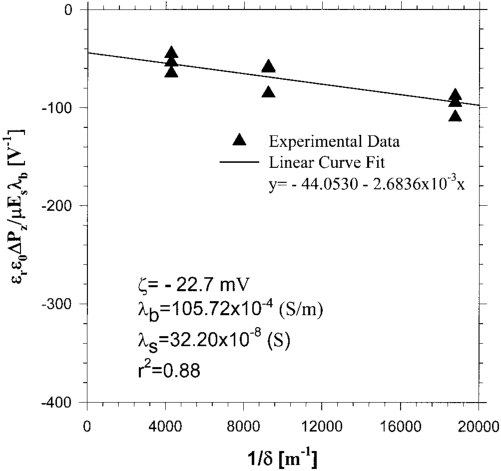
\includegraphics{content/pt1/01-PowerHarvesting/graphics/GuLi_DIUF}
      \caption{\label{fig:Gu_Li_comparison_DUIF}Plot showing measured data from Gu and Li's paper on streaming cells relating the streaming voltage and pressure differential to the channel height with distilled water as the working fluid ~\cite{Gu2000}.}
  \end{figure}

  \begin{figure}
      \centering
      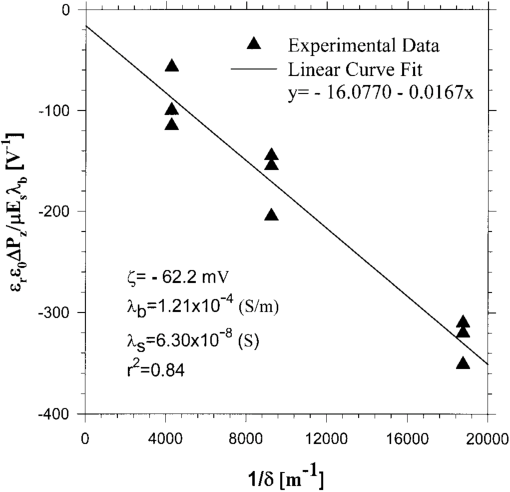
\includegraphics{content/pt1/01-PowerHarvesting/graphics/GuLi_NaCl}
      \caption{\label{fig:Gu_Li_comparison_NaCl}Plot showing measured data from Gu and Li's paper on streaming cells relating the streaming voltage and pressure differential to the channel height with a \SI{1}{\milli\mole} sodium chloride solution as the working fluid~\cite{Gu2000}.}
  \end{figure}

  Their results for three streaming cells are shown here (taken from \cite{Gu2000}) as \cref{fig:Gu_Li_comparison_DUIF,fig:Gu_Li_comparison_NaCl}.
  The first (\cref{fig:Gu_Li_comparison_DUIF}) shows measurements when distilled water is used as the working fluid; the second (\cref{fig:Gu_Li_comparison_NaCl}) shows the measurements for a weak saline solution.
  It is interesting to note that they have what looks to be fairly linear data, although it is hard to tell with only three channel sizes.

  \begin{figure}
      \centering
      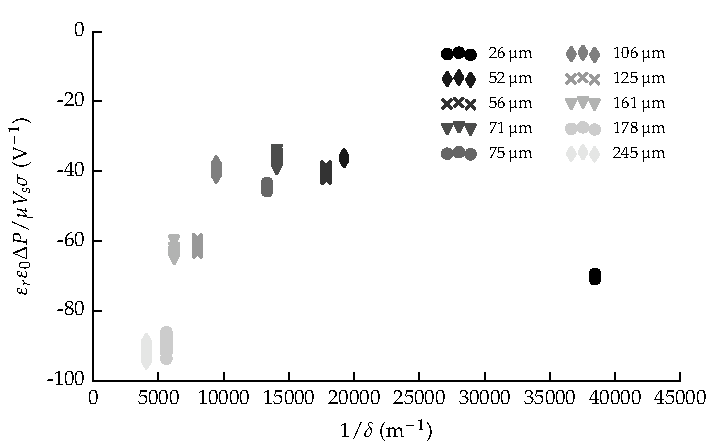
\includegraphics{content/pt1/01-PowerHarvesting/graphics/graph_streamingComparison_gu}
      \caption{\label{fig:streamingCell_scatter_Gu_Li}Scatter plot with results of streaming cell measurements in terms of those made by Gu and Li~\cite{Gu2000} (for comparison).}
  \end{figure}

  By comparison, \cref{fig:streamingCell_scatter_Gu_Li} plots the same variables from measurements taken from the ten streaming cells fabricated here.
  In this graph $\lambda_{b}$ has been replaced with $\sigma$, where both refer to the bulk conductivity of the solution; and $E_{s}$ has been replaced with $V_{s}$, were both refer to the streaming potential.
  The response to variation of channel height is clearly non-linear.
  Their method of finding the zeta potential rests on the following rearrangement:
  \begin{eqnarray}
      \frac{\varepsilon_{r}\varepsilon_{0}\Delta P}{\mu V_{s}\sigma} = \frac{1}{\zeta} + \left( \frac{2\,\lambda}{\zeta \sigma}\right)\,\frac{1}{\delta}
  \end{eqnarray}
  where $\lambda$ is the surface conductivity and $\delta$ is the channel height.
  So as the channel height ($\delta$) tends to infinity, the left hand side tends toward the zeta potential ($\zeta$).
  This notion seems counter intuitive since the zeta potential is defined at the plane of sheer (as shown in \cref{fig:doubleLayer_anatomy}), relative to the solution bulk.
  The equation is stating that no-matter how far you separate the walls, the minimum voltage-pressure gradient you can get is still set by the zeta potential.

  Measurement of the output power generated by the \SI{71}{\micro\meter} streaming cell is promising.
  From this measurement the power transfer curve is evident.
  Referring back to the model presented as \cref{fig:StreamingCell_Schematic-representation}, we can now calculate the channels internal electrical resistance ($R_{cell}$).
  We know from the graph that the maximum power transfer occurred at a current of \SI{33.5}{\nano\ampere} with a streaming voltage of \SI{182}{\milli\volt}.
  Via Ohm's law this equates to a load resistance ($R_{out}$) of \SI{5.43}{\mega\ohm}, which from the maximum power theorem we know must be equal to the cells internal resistance.


\section{Concluding Remarks}
  \label{sect:part1_energyHarvesting_conclusion}

  Conversion of mechanical pumping into electrical energy can be done with narrowly separated plates of glass.
  The conversion efficiency seen here was low, much lower than reported in the literature.
  A channel \SI{1}{\centi\meter} by \SI{3}{\centi\meter} by \SI{71}{\micro\meter} produced \SI{1.5}{\nano\watt} under a pressure differential of \SI{260}{\kilo\pascal}.
  That took \SI{359}{\milli\watt} of pumping power to produce, yielding an efficiency in the order of \SI{0.1}{\micro\percent}.
  Precision engineering, with regards to cell construction, will likely lead to greater efficiency.
  This is based on reports from the literature, where higher efficiency channels utilised much narrower channels.

  Measurements of ten streaming cells were compared to the results published by Gu and Li.
  The linear relationship of Gu and Li between channel height and their plotted parameter could not be reproduced.
  Instead, results showed a highly non-linear relationship as shown in~\cref{fig:streamingCell_scatter_Gu_Li}.
  The gradient of measurement points within the range of channel heights measured by Gu and Li is reversed.
  The reason for the discrepancy is not clear.

  The streaming voltage was found to scale linearly with the applied pressure.
  This could potentially be useful as a means of sensing water flow rates.
  A dual purpose such as power sourcing and flow measurement lends itself well to water metering applications.


  % Edit checkpoint 2015-09-13 19:49


  \chapter{Applicability to Water Metering}
    \label{chap:wirelessWaterMetering}
    %!TEX root = ../../../thesis.tex

% Introduction
Water metering is becoming increasingly common throughout the world~\cite{Chang2012}.
Sourcing and processing drinkable water is an expensive task.
Cheap and reliable methods for reading water meters is important.
As supplies of drinkable water become constrained, volumetric pricing will become increasingly common.
Harvesting energy at the location of metering would eliminate the need for batteries.
If energy harvesting could be done without moving parts, lower component wear should lead to increased service life versus mechanical meters.
This chapter investigates the feasibility of using streaming cell technology as a means of powering electronic water meters.

\Cref{chap:part1_streamingCellHarvesters} discussed electric power generation from streaming cells.
A \SI{0.2}{\micro\percent} conversion efficiency from water flow and pressure was demonstrated.
Also, streaming voltage was found to be directly proportional to the pressure across a cell.
Can that pressure dependence be used as a method to meter water consumption while generating power? Probably.
However, questions like this are only relevant if the harvester is feasible.
Its feasibility is dictated by whether or not it can provide enough energy.
To find that out, the following questions must be answered:
\begin{enumerate}
  \item What quantity of energy is there available to harvest?
  \item What fraction can be harnessed?
  \item How much power do we need?
\end{enumerate}
The second question was answered in \cref{chap:part1_streamingCellHarvesters}, (\SI{0.0002}{\percent}); and the third will be answered in \cref{chap:part1_energyHarvestingRequirements}.
This chapter estimates the quantity of energy available for harvesting in a typical domestic setting.

% Edit checkpoint 2015-09-16 19:14


\section{Trends in Water Metering}

  %
  In New Zealand - Auckland City, Tauranga City, Nelson City, Whangarei District, and the Tasman District have already implemented water metering~\cite{WaterNewZealand2011}.
  For residents of Wellington, New Zealand's capitol city, water metering is optional.
  In metered locations, meter readers must manually read the display of each meter; a long and laborious task.

  % Automatic meter reading systems
  Automatic meter reading systems (AMR) are an alternative method of collecting that data.
  Hamilton City Council is trialling such systems in remote areas in the hopes of adopting them for wide-spread use.
  There are two types of automatic meter reading systems:
  an external reader (with communication interface) that attaches to a compatible meter, or an all-in-one unit that meters and reports usage.
  These systems offer advantages separate from taking away the laborious job of meter reading.
  Increased billing frequency helps customers reduce their consumption by giving more frequent feedback.
  They remove the need to access the customer's property~\cite{Chang2012}.
  Electronic analysis of the meters readings provides an easy way to detect water leaks.

  % Leakages
  It is estimated that \SI{10}{\percent} of post-meter water consumption is due to leakage in the residential sector~\cite{Britton2013}.
  Measuring night-time water flow is a convenient way of estimating flow due to leakage.
  Britton et al.\ show that communicating with customers whose homes showed signs of leakage that a night-time flow reduction of \SI{89}{\percent} is achievable.
  In contrast, a control group's night-time usage increased by over \SI{50}{\percent} during the same time-frame.
  The benefits of automatic water metering are not limited to billing, but improving the network as a whole.

  % Installation
  \begin{figure}
    \centering
    \includegraphics[width=0.9\textwidth]{content/pt1/02-WirelessWaterMeter/graphics/meter}
    \caption{\label{fig:Photo_DomesticWaterMeter}Photo showing a domestic water meter, and installation, (Kent PSMT 25mm) typical of an Auckland residential area.}
  \end{figure}
  Domestic water meters are typically installed at a property's boundary in a plastic box set into the ground.
  An installation typical for an Auckland residential area is shown in \cref{fig:Photo_DomesticWaterMeter}.
  The meter is installed over five meters into the property from the road-side.
  It is not feasible to connect it to a source of power because of its location.
  No commercially available domestic energy harvesting water meters, suitable for burial, exist on the market as of January 2015.

  % Approaches
  \begin{figure}
    \centering
    \label{fig:Photo_waterwareMeter}
    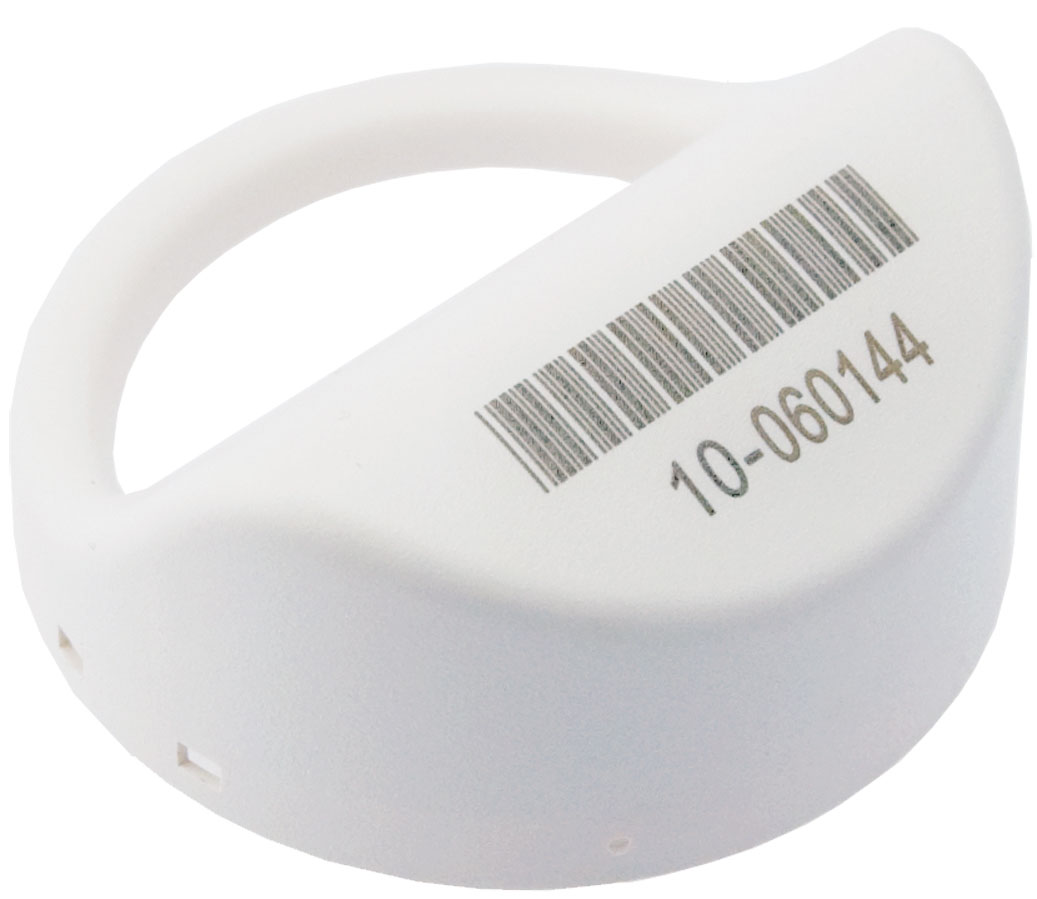
\includegraphics[width=0.5\textwidth]{content/pt1/02-WirelessWaterMeter/graphics/hydro-WMBUSWLESSM}
    \caption[Photo of a wireless transmitting module from Waterware NZ.]{
      Photo of a wireless transmitting module from Waterware NZ.
      The device attaches to a compatible water meter and contains its own battery~\cite{BMeters2014}.
    }
  \end{figure}
  A common configuration for wireless automatic meter reading is to have a reader/transmitter device that is separate to the meter itself.
  Such a device usually attaches to the meter's display or has a wire connecting it to the meter.
  Being detachable and tamper-proof means it must be powered by batteries.
  A commonly stated battery life for such units is ten years~\cite{BMeters2014}, close to a battery's shelf-life.
  We investigate the possibility of replacing these batteries with a streaming cell based energy harvester.
  A harvester removes the need for batteries, but needs to be plumbed into the water feed.
  It if for this reason that the resulting device would most likely replace the meter, as opposed to being an attachment.


  \section{Mechanical Design of a Harvester}

    % Issuse with scaling
    In \cref{chap:part1_streamingCellHarvesters}, energy was converted between fluid-mechanical to electrical using a single channel.
    Harvesting for electronic water meters will require more energy than that channel could produce.
    There are multiple ways of scaling the streaming cell design used in \cref{chap:part1_streamingCellHarvesters}.
    The channel can be made wider, doubling the width will double the output power;
    multiple channels can be stacked together, multiplying the output by the number of channels formed.
    Scaling the harvester is not considered a problem, but the pressure drop it develops is.
    High fluid resistance is inevitable since practical efficiencies are only obtained when the internal dimensions are small.

    % Intended harvester design
    \begin{figure}
      \centering
      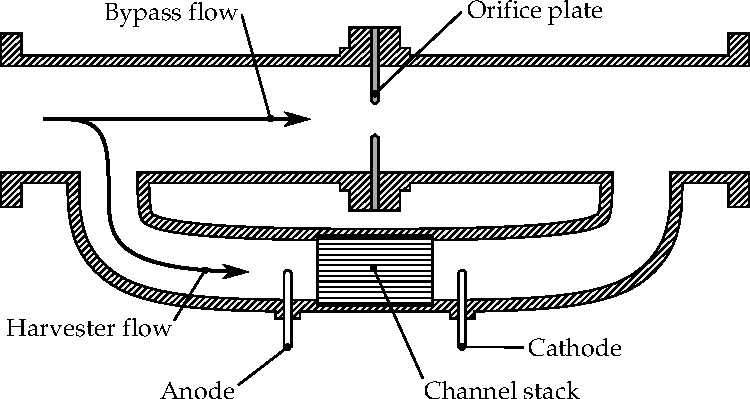
\includegraphics[width=0.9\textwidth]{content/pt1/02-WirelessWaterMeter/graphics/harvester}
      \caption{\label{fig:Diagram_harvester}Diagram showing the intended design of streaming cell harvester suitable for domestic connection.}
    \end{figure}
    To control the pressure drop across the harvester, the mechanical design shown in~\cref{fig:Diagram_harvester} is proposed.
    It gives the capability of controlling the hydrodynamic resistance of the unit as a whole by means an orifice plate.
    The plate sits in the ``main line'' causing a pressure differential in proportion to the flow rate.
    An orifice plate with a hole equal in diameter to the main pipe causes no pressure differential as it causes no flow obstruction.
    Conversely, a plate without a hole forces all liquid through the harvester, causing the maximum pressure differential.
    Using an appropriate sized orifice plate, the customer will be unaware of the harvester's presence and a suitable pressure differential will be developed.
    For the sake of analysis we assume the orifice plate will be sized to match the pressure loss of a mechanical meter.
    This assumption means the amount of harvestable energy is equal to the amount dissipated in a mechanical water meter.
    The following section quantifies the amount of energy a water meter dissipates over an average week in a typical Auckland home.


  \section{Quantifying Harvestable Energy}
  \label{sect:part1-WirelessWaterMeter-QuantifyingHarvestableEnergy}

    % Recap
    Using a bypass pipe with an orifice plate, the pressure drop across a streaming cell energy harvester can be controlled.
    The following calculations are based on the assumption that the streaming cell energy harvester will be set to collect the same amount of energy currently lost inside a typical mechanical meter.

    % Water usage information
    \begin{table}
      \centering
      \begin{tabular}{r l|r|r|l}
        Item                    & Measurement & Summer & Winter & Unit\\
        \hline\hline
        \multirow{4}{*}{Shower} & Duration    & 6.6    & 7.0    & minutes\\
                                & Volume      & 50.0   & 52.5   & litres\\
                                & Flow        & 8.1    & 8.0    & litres/minute\\
                                & Frequency   & 0.9    & 0.9    & /person/day\\
        \hline
        \multirow{2}{*}{Washing}& Volume      & 122    & 123    & litres\\
                                & Frequency   & 0.35   & 0.36   & /person/day\\
        \hline
        \multirow{2}{*}{Toilet} & Volume      & 6.6    & 6.8    & litres\\
                                & Frequency   & 4.9    & 4.5    & /person/day\\
      \end{tabular}
      \caption{
          \label{tab:consumption_figures}
          Average usage characteristics for a shower, washing machine and toilet.
          Data obtained from~\cite{Heinrich2008}.
      }
    \end{table}
    Heinrich monitored water consumption of 51 homes throughout Auckland in 2008~\cite{Heinrich2008}.
    His report shows the majority of domestic water is consumed by the shower (\SI{30}{\percent}), washing machine (\SI{27}{\percent}) and toilet (\SI{20}{\percent}).
    Together these account for over \SI{75}{\percent} of domestic water consumption.
    Data from \cref{tab:consumption_figures} was used to build a typical water usage profile.
    Heinrich published a similar report in 2007 that contained water flow profiles, the flow profile of the toilet has been taken from that report~\cite{Heinrich2007}.

    % Profile
    \begin{figure}
      \centering
      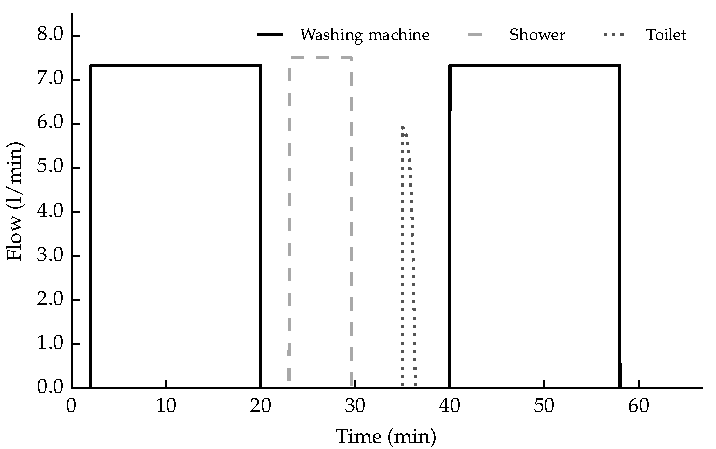
\includegraphics[width=\linewidth]{content/pt1/02-WirelessWaterMeter/graphics/graph_profile}
      \caption[Graph showing a water consumption profile of constructed instances of washing machine use, a shower and a toilet flush.]{
          Graph showing a water consumption profile of constructed instances of washing machine use, a shower and a toilet flush.
          The washing machine's wash and rinse cycles are separated in time.}
      \label{fig:profileSample}
    \end{figure}
    \Cref{fig:profileSample} shows the flow rates for each of the three items considered (toilet, shower and washing machine).
    Volumes for each of the events, and flow profile of the toilet, match the measurements reported by Heinrich.
    Specifically, the total volumes for each are: \SI{122}{\litre}, \SI{49.5}{\litre} and \SI{6.22}{\litre} for the washing machine, shower and toilet respectively.

    % Pressure loss
    \begin{figure}
        \centering
        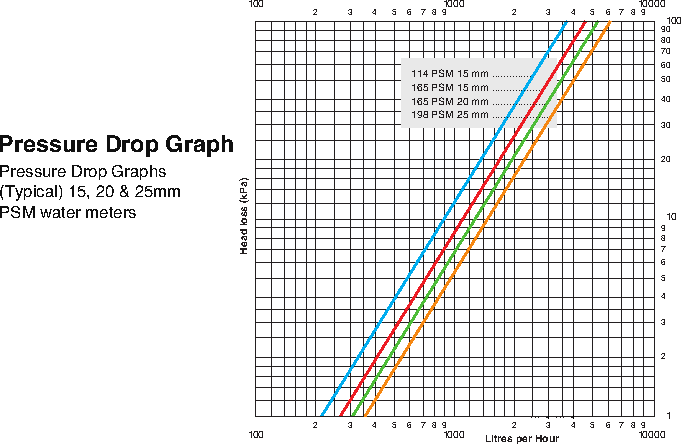
\includegraphics[width=\linewidth]{content/pt1/02-WirelessWaterMeter/graphics/Kent-PSM-HeadLoss}
        \caption{
            \label{fig:headloss}
            Log-log graph showing the pressure developed across the Kent PSM series mechanical water meters. Taken from~\cite{Elster2008}.
        }
    \end{figure}
    The Kent 25-PSMT series mechanical water meter is the most commonly installed water meter in the Auckland district~\cite{WatercareNewZealand2014}.
    \Cref{fig:headloss} shows the head-loss, or pressure differential, versus flow rate for the Kent PSM range of meters.
    The following equation was created to describe the trace representing the \SI{25}{\milli\meter} PSMT meter:
    \begin{equation}
        \Delta P = e^{3.725\thinspace log(flow) - 9.5}
        \label{eqn:Flow_to_pressure_25mmPSMT}
    \end{equation}
    \begin{figure}
        \centering
        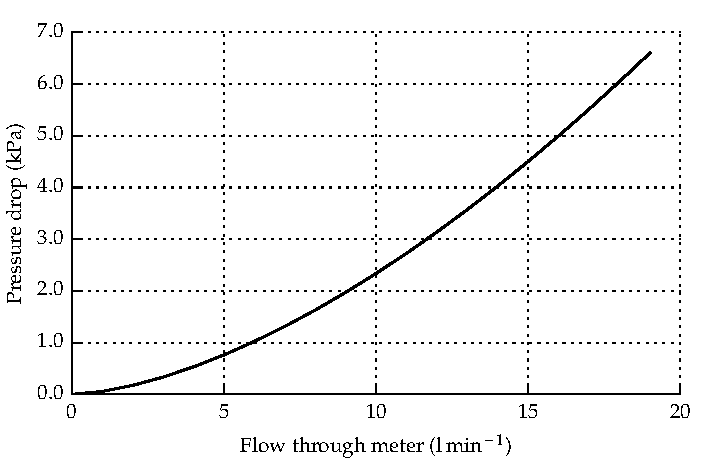
\includegraphics[width=\linewidth]{content/pt1/02-WirelessWaterMeter/graphics/graph_pressureLoss}
        \caption{Graph showing fitted curve to the pressure loss graph presented as \cref{fig:headloss}.}
        \label{fig:headloss_fit}
    \end{figure}
    \Cref{eqn:Flow_to_pressure_25mmPSMT} is plotted in \cref{fig:headloss_fit} on linear scales.

    % Calculating power loss
    Knowing the pressure differential as a function of flow provides a means of converting between flow and power dissipation.
    Like an electrical resistance, power dissipated by a fluid-flow obstruction is the product of the difference in driving force across the resistance and the flow through it.
    In this case the driving force is pressure and the flow is volumetric.
    \begin{align}
      \label{eqn:pressure_flow_to_power}
      power &= pressure \cdot flow\nonumber \\
      Watt &= Pascal \cdot \frac{cubic meter}{second}\nonumber \\
      \frac{kg\cdot m^{2}}{s^{3}} &= \frac{kg}{m\cdot  s^{2}} \thinspace \frac{m^{3}}{s}
    \end{align}
    \Cref{eqn:pressure_flow_to_power} shows the units that will be used to determine power dissipation and ensures they balance.
    \begin{figure}
        \centering
        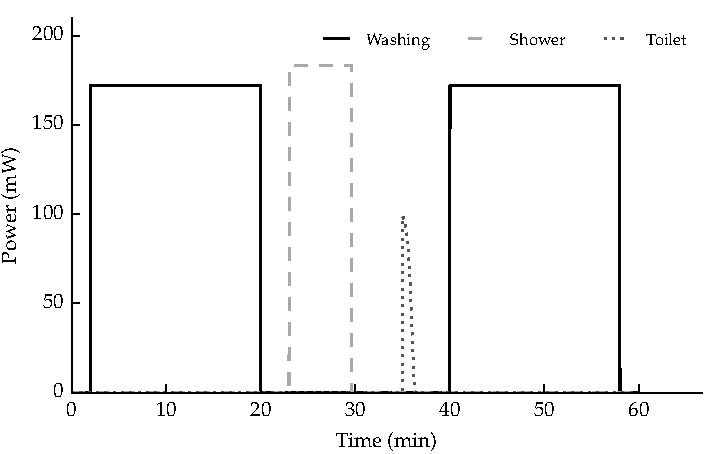
\includegraphics[width=\linewidth]{content/pt1/02-WirelessWaterMeter/graphics/graph_harvest}
        \caption{Graph of calculated power dissipation in a typical domestic mechanical water meter for each of the sample profile events.}
        \label{fig:powerDissipated_meter}
    \end{figure}
    \begin{table}
      \centering
      \begin{tabular}{r|r}
          Washing & \SI{172}{\joule}\\
          Shower  & \SI{72.6}{\joule}\\
          Toilet  & \SI{5.07}{\joule}
      \end{tabular}
      \caption{
        \label{tab:energy_dissipation_figures}
        Calculated energy dissipation within a mechanical water meter for a single washing machine cycle, shower and toilet use.
      }
    \end{table}
    Running the profiles of \cref{fig:profileSample} through \cref{eqn:Flow_to_pressure_25mmPSMT}, with relevant unit conversions, yields~\cref{fig:powerDissipated_meter}.
    It shows the power dissipated within the water during each event.
    Integrating each trace with respect to time gives the total energy lost over the course of each.
    Those energy figures are provided in~\cref{tab:energy_dissipation_figures}.

    % Total energy available
    \begin{figure}
        \centering
        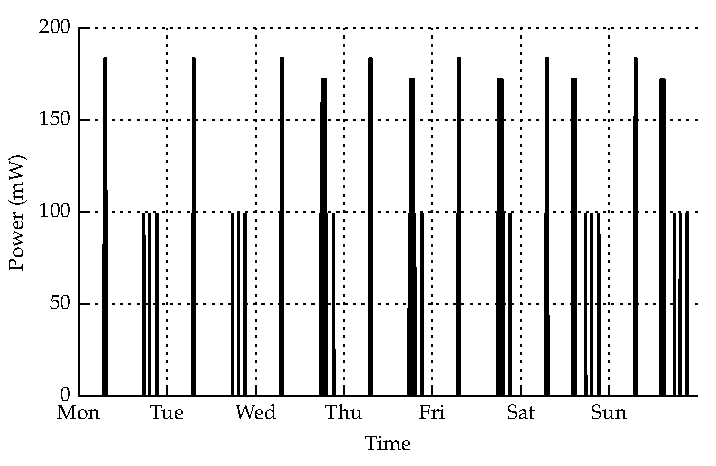
\includegraphics[width=\linewidth]{content/pt1/02-WirelessWaterMeter/graphics/graph_profileEnergy}
        \caption{
          \label{fig:profile_powerDissipation}
          Graph of power dissipation within a mechanical water meter over a week for a two occupant dwelling.
        }
    \end{figure}
    Average use frequencies for each event type are reported by Heinrech and are shown earlier in~\cref{tab:consumption_figures}.
    Using these figures, and by selecting appropriate times of day, an energy dissipation profile representative of one week was constructed.
    Five uses of a washing machine, fourteen showers, and fifty six toilet flushes occur during this time.
    This profile is shown as~\cref{fig:profile_powerDissipation}.
    The profile fits usage figures of a home having two occupants, although most homes have more than two occupants.
    A systematic bias toward underestimating typical water usage has been used where possible.
    This underestimation also occurs by not including water use by means other than washing machines, showers or toilets.
    The intention is that the feasibility of harvesting, if the results showed near a possibility, would be more robust in light of these biases.
    \begin{table}
      \centering
      \begin{tabular}{r|r}
          Washing & \SI{860}{\joule}\\
          Shower  & \SI{1020}{\joule}\\
          Toilet  & \SI{283.9}{\joule}
      \end{tabular}
      \caption{
          \label{tab:energy_dissipation_total_figures}
          Calculated total energy dissipation over a period of one week within a mechanical water meter for typical use of a washing machine, shower and toilet.
      }
    \end{table}
    \Cref{tab:energy_dissipation_total_figures} combines the energy dissipation for each event type over a week.
    The total energy dissipated in the meter during such a week is \SI{2.16}{\kilo\joule}.
    Daily energy available is expected to fluctuate due to sporadic use of the washing machine in most homes.
    Ignoring washing machine use, indicative of weekday consumption, the quantity of harvestable energy is expected to be about \SI{280}{\joule} per day.

    % Summary
    Knowing the quantity of energy available to a harvester is a key factor determining its feasibility.
    The efficiency of converting energy into the electrical domain was measured in~\cref{chap:part1_streamingCellHarvesters} and was found to be \SI{0.2}{\micro\percent}.
    Based on that figure the measured cell would collect \SI{560}{\nano\joule} of energy per day from a two person home.
    Energy output that low is unlikely to be sufficient for automatic meter reading.
    The literature indicates the efficiency measured in~\cref{chap:part1_streamingCellHarvesters} was low.
    It may still be possible to close the gap between what we can produce and what we need.
    The amount of energy required to run an electronic water meter is estimated next.

    % Edit checkpoint 2015-09-16 19:48


  \chapter{Energy Requirements}
    \label{chap:energyRequirements}
    %!TEX root = ../../../thesis.tex

The amount of energy lost in a mechanical water meter has been estimated, as has the fraction of that energy which can be harnessed.
Now, the amount of energy required to operate an electronic water meter is sought.
This estimation will reveal how much further the cells built earlier would need to be improved to be viable.

\section{Microcontrollers}

  Central to the operation of an electronic water meter is the microcontroller (MCU).
  The primary function of the microcontroller is to read and log the amount of water consumed by the meter.
  The programme contained on the controller will also decide when to transmit that data and monitor energy usage.
  It is therefore a key component and is expected to consume the majority of energy.

  This chapter compares the power consumption and operational efficiencies of six low power MCUs deemed suitable for use in electronic metering applications.
  These microprocessors are low power, general purpose, 8-bit processors from Microchip, Atmel, and Freescale.
  Each of the microprocessors will have their energy consumption recorded while carrying out various functions over a range of supply voltages.
  Such measured functions are analogue-to-digital conversion, non-volatile memory writes, processing, and sleeping.


  \subsection{Selection of low power processors}

    \begin{sidewaystable}
      \begin{centering}
        \begin{tabular}{|l|l|l|l|l|l|l|l|}
        \cline{2-8}
        \multicolumn{1}{l|}{} & PIC16F1827  & PIC16F887  & PIC16F688  & PIC12F675  & ATtiny25V  & ATtiny13V  & MC9S08QG8 \tabularnewline
        \hline
        Vdd (min)  & 1.8  & 2.0  & 2.0V  & 2.0  & 1.8  & 1.8  & 1.8 \tabularnewline
        Vdd (max)  & 5.5  & 5.5  & 5.5V  & 5.5  & 5.5  & 5.5  & 3.6 \tabularnewline
        I (sleep)  & 30nA  & 50nA  & 50nA  & 1nA  & 100nA & <100nA & 450nA\tabularnewline
        CLOCK (min)  & 31kHz  & 31kHz & 31kHz & 31kHz & 16kHz & 16kHz & 1MHz \tabularnewline
        CLOCK (max)  & 32MHz  & 8MHz  & 8MHz  & 4MHz  & 16MHz & 9MHz  & 10MHz\tabularnewline
        EEPROM  & 256B  & 256B  & 256B  & 128B  & 128B  & 64B  & \dag{}\tabularnewline
        Serial  & USI  & USI  & USI  & --  & USI  & --  & USI \tabularnewline
        USART  & UART  & UART  & UART  & --  & --  & --  & -- \tabularnewline
        ADC  & 10bit  & 10bit & 10it  & 10bit & 10bit & 10bit & 10bit\tabularnewline
        \hline
        \end{tabular}
      \end{centering}

      \begin{centering}
      \dag Has 8,192 bytes of software programmable flash (16 pages of 512 bytes each).
      \end{centering}

      \begin{centering}
      \ddag Has 256 bytes of software programmable flash (4 pages of 64 bytes each).
      \end{centering}

      \caption{\label{tab:MCUfeaturecomparison} Feature comparison of benchmarked microprocessors.}
    \end{sidewaystable}

    The following processors were chosen from the three chosen manufacturers.
    \begin{itemize}
    \item Microchip PIC16F1827
    \item Microchip PIC16F688
    \item Microchip PIC12F675
    \item Atmel ATtiny25V
    \item Atmel ATtiny13V
    \item Freescale MC9S08QG8
    \end{itemize}
    A basic feature comparison of the MCU selection is shown in table \ref{tab:MCUfeaturecomparison}.





% \section{Power consumption}

% Each of the MCUs were programmed to carry out various tasks which
% were performed over their specified range of operating voltages and
% operating frequencies. While the chips where carrying out these tasks
% their power consumption was measured by an Agilent E5270B Precision
% Mainframe via a PC and a Tektronix MSO 4054 Oscilloscope for timing
% purposes. Details on how each of the tests where carried out, as well
% as raw data, can be found in appendix %\ref{Appendix:Measurements} .


  \subsection{Benchmarking power consumption}

    It is important to ensure that each processor is operated so as to minimise power consumption, which meant taking certain precautions.
    Spare pins were set as outputs and tied to Vdd with \SI{10}{\kilo\ohm} resistors.
    Unused peripherals were disabled including any watchdog timers and brownout detection circuitry.
    To allow more accurate sleep current measurements, the chips were placed in a chip carrier with \SI{10}{\kilo\ohm} resistors soldered between the general purpose pins and Vdd.
    The chip and carrier was washed in isopropyl alcohol and dried before being suspended by connections to the measurement device.
    This step minimises leakage current between the pins due to oils and dirt that may be transferred by touching or resting on a table.
    Measurements were carried out using the Agilent E5270B Precision Measurement Mainframe.
    This device has been used for most other measurement situations throughout this thesis for its high impedance inputs and measurement accuracy.


    \subsubsection{Sleep mode}


      \begin{figure}
        \centering
        \includegraphics{content/pt1/03-EnergyRequirements/graphics/Graph_All_Sleeping_Current}
        \caption{\label{fig:All_Sleep_Current}Graph showing current consumed by MCUs in sleep mode versus supply voltage.}
      \end{figure}

      A microprocessor in sleep mode is essentially powered off, the difference being that volatile data is preserved.
      In order to consume as little power as possible an MCU should spend as much time in sleep mode as possible.
      The power consumption while sleep states will determine a large part of the water meters overall energy requirements.

      \Cref{fig:All_Sleep_Current} shows the amount of current consumed by each MCUs while in their deepest sleep states.
      Surprisingly, the PIC16F1827 consumes the most current in this state, almost one thousand times more than the specified sleep current of \SI{30}{\nano\ampere}\cite{PIC16F1827}.
      The Freescale MC9S08QG8 consumed energy at an average of 11\% higher than specified \cite{MC9S08QG8}.
      Both the Atmel ATtiny13V and ATtiny25V fell within their specification, \cite{AtmelATtiny13,AtmelATtiny25} respectively.
      The Microchip PIC12F675 fell within specification\cite{PIC12F675} and was clearly ahead in terms of minimum current draw during sleep.

      There appears to be a trade-off between the two Atmel processors in the way of minimum power consumption and minimum response to Vdd.
      The ATtiny13V required approximately 2.7 times less power than the ATtiny25V at 1.8V, but above 2.5V the ATtiny25V is more draws less current.

      As the PIC16F1827 was so far off its specified value, measurements were repeated numerous times using code written in both assembler and HI-TECH C.
      A total of five different processors were tried, all giving the same result.
      All steps outlined in the PIC16F1827's datasheet to reduce power consumption had been followed.


    \subsubsection*{Disclaimer on processing}


      Measuring the amount of power required to process information is complicated.
      The way each chip carries out processing operations internally can differ from one another, even though all produce the same result.

      \begin{table}
        \centering
        \begin{tabular}{|c|c|}
          \cline{2-2}
          \multicolumn{1}{c|}{} & Instructions\tabularnewline
          \hline
          PIC16F1827 & 53\tabularnewline
          \hline
          PIC16F688 & 35\tabularnewline
          \hline
          PIC12F675 & 35\tabularnewline
          \hline
          ATtiny25V & 120\tabularnewline
          \hline
          ATtiny13V & 120\tabularnewline
          \hline
          MC9S08QG8 & 145\tabularnewline
          \hline
        \end{tabular}
        \caption{\label{tab:Number-of-instructions}Number of instructions in microprocessor instruction set for benchmarked microprocessors.}
      \end{table}


      \begin{algorithm}
        \begin{lstlisting}
        if (danger >= 5) flight();
        else fight();
        \end{lstlisting}
        \caption{\label{alg:Simple-C-code-representation}Simple C-code representation of a branch instruction.}
      \end{algorithm}


      To illustrate, algorithm \ref{alg:Simple-C-code-representation} shows a simplified programme.
      To determine  the programme's outcome the processor must first evaluate whether `danger' is greater than or equal to five.
      Then it will either branch to the function `fight' or continue on to execute the function `flight'.

      \begin{algorithm}
        \begin{lstlisting}
        load 5 into register 001
        load danger into register 002
        branch-if-greater-or-equal 001 002 flight_call
        call-subroutine fight
        jump-to continue
        [flight_call]
        call-subroutine flight
        [continue]
        \end{lstlisting}
        \caption{\label{alg:Psudo-machine-code1}Pseudo machine-code representation
        of a branch instruction.}
      \end{algorithm}

      \begin{algorithm}
        \begin{lstlisting}
        load danger into register 001
        subtract-from-register 001 5
        branch-if-minus 001 fight_call
        call-subroutine flight
        jump-to continue
        [fight_call]
        call-subroutine fight
        [continue]
        \end{lstlisting}
        \caption{\label{alg:Psudo-machine-code2}Pseudo machine-code representation of an alternative branch instruction.}
      \end{algorithm}


      Algorithms \ref{alg:Psudo-machine-code1} and \ref{alg:Psudo-machine-code2} demonstrate two different ways of implementing \ref{alg:Simple-C-code-representation} using pseudo machine-code.
      The decision of which to use is made by the compiler, which \emph{should} take the instructional efficiency of the specific MCU into account.
      This is an overly simplistic example, but it illustrates that there are multiple paths leading to the same result.
      Importantly, not all of those paths require the same amount of effort on the processor's behalf.
      This means that the compiler's ability to optimise code efficiently plays a role in determining the overall performance of the chip.
      This also means that the programmer should not be concerned with instructional efficiency as the compiler should transform C-code into machine code that best suits the target MCU.

      Another factor in processing efficiency comes down to the number of different instructions it is capable of.
      The list of instructions a processor is capable of is called its instruction set.
      Most 8-bit MCUs are based on reduced instruction set computing (RISC) architecture, as opposed to complex instruction set computing (CISC).
      When compared to a CISC based CPU, a RISC based chip is simpler and therefore usually cheaper to produce and simpler to program.
      However, ``Instruction traces from CISC machines consistently show that few of the available instructions are used in most computing environments''\cite{ComputerArch}, meaning that many of the extended operations in CISC designs are underutilised.
      Processors with smaller instruction sets are capable of achieving the more complex operations by chaining multiple instructions together.
      This means that processors with smaller instruction sets may take longer to execute certain instructions.
      Finally, the frequency of a microprocessor isn't necessarily the frequency at which it performs operations, although sometimes it is.
      For instance, the Atmel and Freescale microprocessors perform one instruction per clock cycle, whereas the Microchip processors perform one instruction every four clock cycles.


    \subsubsection{Processing}

      \begin{figure}
        \centering
        \includegraphics{content/pt1/03-EnergyRequirements/graphics/Graph_PIC16F1827_Clock_Power}
        \caption{\label{graph:CLK_POWER_16F1827}Graph showing power consumed by the PIC16F1827 while processing versus supply voltage.}
      \end{figure}

      \begin{figure}
        \centering
        \includegraphics{content/pt1/03-EnergyRequirements/graphics/Graph_PIC16F688_Clock_Power}
        \caption{\label{graph:CLK_POWER_16F688}Graph showing power consumed by the PIC16F688 while processing versus supply voltage.}
      \end{figure}

      \begin{figure}
      \centering
        \includegraphics{content/pt1/03-EnergyRequirements/graphics/Graph_PIC12F675_Clock_Power}
        \caption{\label{graph:CLK_POWER_12F675-1}Graph showing power consumed by the PIC12F675 while processing versus supply voltage.}
      \end{figure}

      \begin{figure}
      \centering
        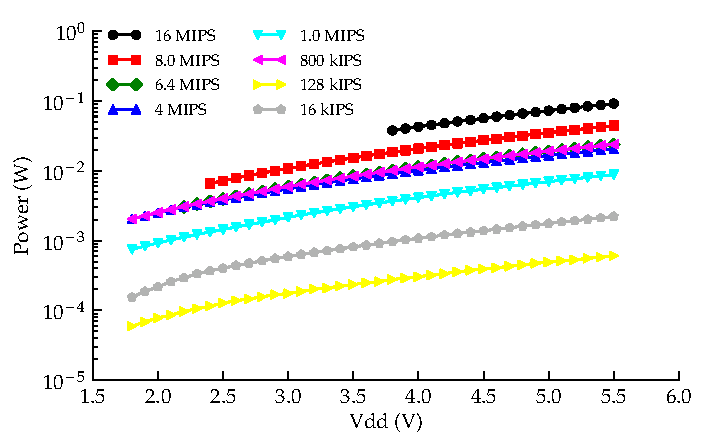
\includegraphics{content/pt1/03-EnergyRequirements/graphics/Graph_ATtiny25V_Clock_Power}
        \caption{\label{graph:CLK_POWER_ATtiny25V}Graph showing power consumed by the ATtiny25V while processing versus supply voltage.}
      \end{figure}

      \begin{figure}
        \centering
        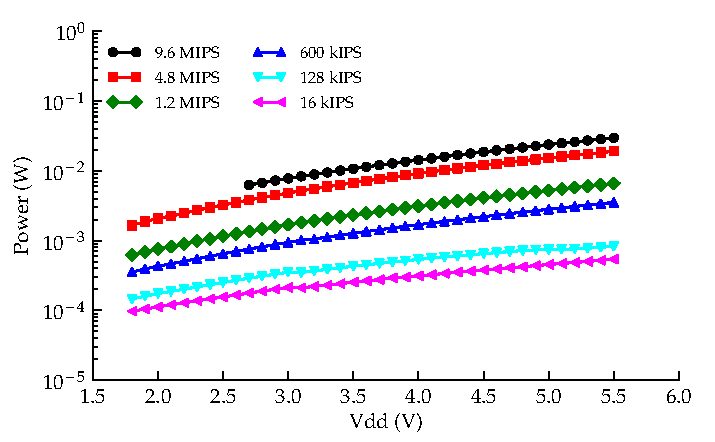
\includegraphics{content/pt1/03-EnergyRequirements/graphics/Graph_ATtiny13V_Clock_Power}
        \caption{\label{graph:CLK_POWER_ATtiny13V}Graph showing power consumed by the ATtiny13V while processing versus supply voltage.}
      \end{figure}

      \begin{figure}
        \centering
        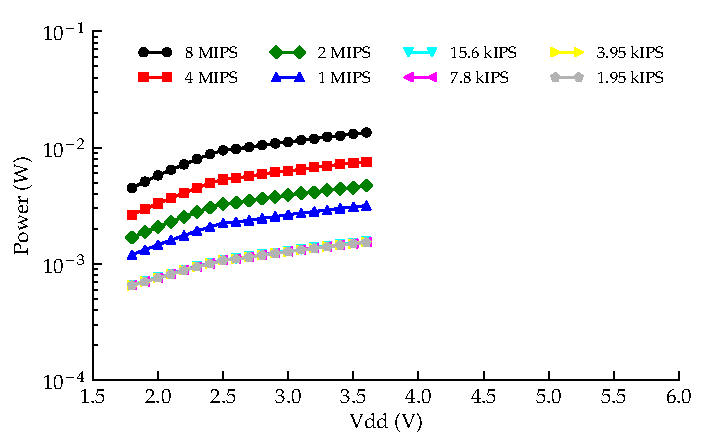
\includegraphics{content/pt1/03-EnergyRequirements/graphics/Graph_MC9S08QG8_Clock_Power}
        \caption{\label{graph:CLK_POWER_MC9S08QG8}Graph showing power consumed by the MC9S08QG8 while processing versus supply voltage.}
      \end{figure}

      Results in this section are expressed in terms of instructions per second (IPS).
      The Microchip PIC16F1827 displayed the lowest energy usage with \SI{10}{\micro\ampere} while clocking \SI{7.75}{\kilo IPS} (as shown in \cref{graph:CLK_POWER_16F1827}).
      Microchip MCUs complete one instruction every four clock cycles, so the \SI{7.75}{\kilo IPS} actually corresponds to a standard clock frequency of \SI{31}{\kilo\hertz}.

      % Edit checkpoint 2015-09-17 18:59

      \Cref{graph:CLK_POWER_16F688} shows that the PIC16F688 consumes less power than the PIC16F1827 at low voltages for the same instruction rates (except at 7.75kIPS).
      There appears to be a flatter response in power consumption with respect to Vdd in the PIC16F1827.
      Again, this appears to be a similar trade-off to what was mentioned earlier (in \cref{fig:All_Sleep_Current}) with the Atmel chips.

      The PIC12F675 (\cref{graph:CLK_POWER_12F675-1}) used approximately the same power as the PIC16F688 (\cref{graph:CLK_POWER_16F688}) for its \SI{1}{\mega IPS} trace.
      \Cref{graph:CLK_POWER_ATtiny25V,graph:CLK_POWER_ATtiny13V} show both Atmel MCUs having similar requirements.
      The MC9S08QG8, although being able to clock the slowest, performed very poorly at low frequencies.
      At \SI{1.95}{\kilo IPS} it consumed approximately the same amount of power as the Microchip MCUs operating at \SI{1}{\mega IPS}.

      Overall, the PIC16F1827 gives the widest range of power consumption options, with the ATtiny25V offering similar performance options.

    \subsubsection*{Joules of energy consumed per instruction cycle\label{sub:Joules-of-energy}}

      A convenient, and more insightful way to interpret the previous processing power consumption graphs is to calculate the energy spent per instruction performed.
      The energy cost of an instruction cycle can be calculated using equation \ref{eq:JPI calculation}.

      \begin{equation}
      E_{i}=\frac{I\times Vdd}{f_{i}}\label{eq:JPI calculation}
      \end{equation}
      where $E_{i}$ is the number of joules consumed per instruction, $I$ is the current draw, $Vdd$ is the input voltage and $f_{i}$ is the instruction frequency.

      Figure \ref{fig:Per-instruction-cycle} compares the most energy efficient operating conditions of each of the tested chips.
      What is most interesting about this graph is the high degree of overlap.
      Also, the greater efficiencies occur at high operating frequencies.
      A simple rule of thumb for selecting the most power efficient operating frequency based on these results is to choose the highest frequency where the MCU can operate over its full input voltage (Vdd) range.
      For comparison, figure \ref{fig:Per-instruction-ATtiny13V} shows the trade-off made when selecting a higher frequency, which is typical across the range of MCUs tested.

      \begin{figure}
      \begin{centering}
      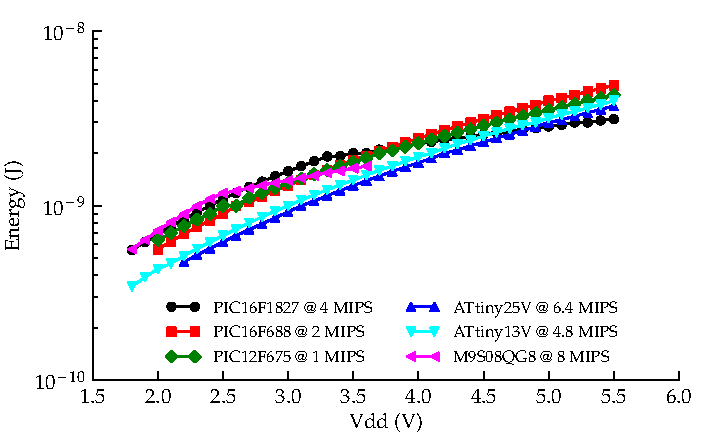
\includegraphics{content/pt1/03-EnergyRequirements/graphics/Graph_All_Clock_JPI}
      \par\end{centering}

      \protect\caption{\label{fig:Per-instruction-cycle}Graph showing instruction cycle energy consumption for each MCU versus supply voltage.}
      \end{figure}
      \begin{figure}
      \begin{centering}
      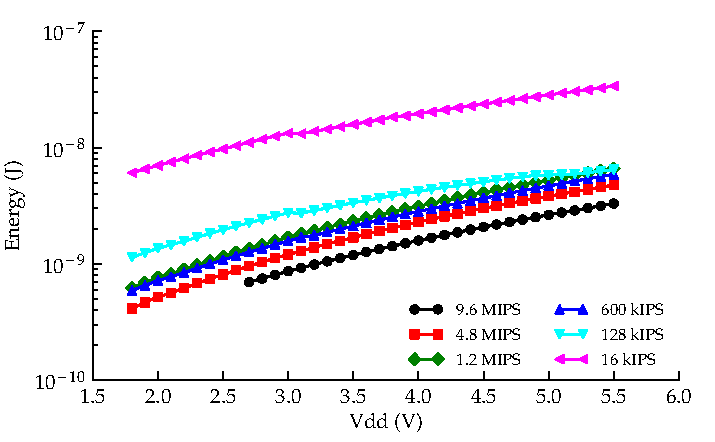
\includegraphics{content/pt1/03-EnergyRequirements/graphics/Graph_ATtiny13V_Clock_JPI}
      \par\end{centering}

      \protect\caption{\label{fig:Per-instruction-ATtiny13V}Graph showing instruction cycle energy consumption of the ATtiny13V versus supply voltage.}
      \end{figure}



    \subsubsection{Instruction efficiency}

      \begin{algorithm}
        \begin{lstlisting}
          unsigned short lfsr = 0xACE1u;
          unsigned period = 0;
          do {
            lfsr = (lfsr >> 1) ^ (-(lfsr & 1u) & 0xB400u);
            ++period;
          } while(lfsr != 0xACE1u);
        \end{lstlisting}
        \caption{\label{alg:Benchmarking-algorithm}Benchmarking algorithm}
      \end{algorithm}

      Calculating the amount of energy consumed per instruction only shows part of processor efficiency.
      The amount of processing done per instruction is not taken into account in such measurements.
      Some MCUs have extra instructions that are designed to help speed up code execution by combining commonly used groups of instructions.
      To shed light on instructional efficiency, the number of instructions each of the processors takes to complete a benchmark function is found.
      This will allow for a more accurate representation of execution efficiency.
      The function used to benchmark each of the processors is a linear feedback shift register based pseudo-random number generator \cite{Wikipedia2015}.
      It is well suited to an 8-bit microprocessor as it requires no complex math functions, uses little memory and has a well defined end.
      The code for this function is shown as \cref{alg:Benchmarking-algorithm}.
      It starts with a 16-bit number and runs it through the linear feedback register in a tight loop until the initial value of the 16-bit feedback register is produced again.
      This function steps through every possible combination of bits possible in a 16-bit number (except for 0 and 65535) in a pseudo-random order before exiting the loop.
      The function combines the exclusive-OR (XOR), bit shifting, bitwise AND, increment a value and numerical comparison operations in a tight loop.
      The benchmarking function was compiled and run on each of the MCUs operating at a range of supported frequencies.

      \begin{figure}
          \begin{centering}
              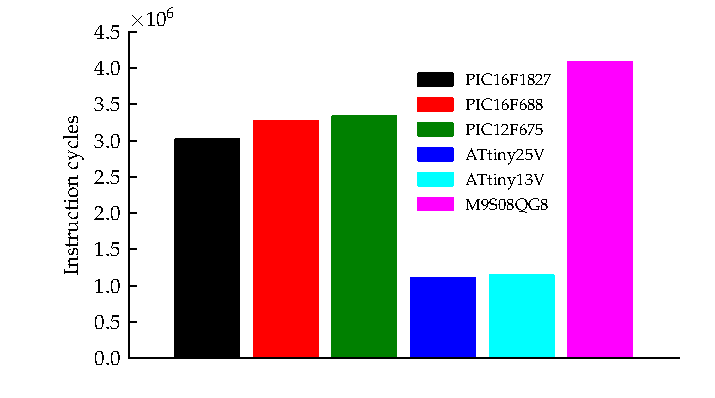
\includegraphics{content/pt1/03-EnergyRequirements/graphics/Graph_All_Clock_Benchmark}
          \end{centering}
          \protect\caption{\label{fig:GraphBar_All_Benchmark}Graph showing the number of instruction cycles taken to complete a benchmark routine for each MCU.}
      \end{figure}

      To determine the instructional efficiency, the code was set to toggle the state of a digital output pin.
      The toggle frequency of that pin was recorded using a Tektronix MSO 4054 oscilloscope.
      The number of instruction cycles each chip took to complete the benchmark was deduced by multiplying the time taken to complete the benchmark by the instruction cycle frequency.
      The results of the benchmark are shown in \cref{fig:GraphBar_All_Benchmark}.
      To calculate the number of instruction cycles taken by the Microchip family of processors, one quarter of the chip's operation frequency was used.
      This meant that the number of clock cycles consumed was four times higher.
      It is clear from \cref{fig:GraphBar_All_Benchmark} that the Atmel (ATtiny25V and ATtiny13V) microprocessors are by far the most efficient microprocessor in terms of executing code using a minimum number of instructions of the selection.
      The reason for this is most probably due to the larger instruction set and higher compiler optimisation.



    \subsubsection{Non-volatile memory}

      In order for a microprocessor to keep information about its current state and recorded data in the event of power loss it must write to non-volatile memory.
      Non-volatile memory is implemented as either electrically erasable and programmable read only memory (EEPROM) or Flash memory.
      Flash memory is similar to EEPROM with the exception that it must be erased in large blocks, or pages, before it can be written to.
      All of the tested MCUs have on-board EEPROM with the exception of the MC9S08QG8 which has flash memory instead.
      Table \ref{tab:MCUfeaturecomparison} shows the amount of non-volatile memory space available on each of the chips.

      \begin{figure}
        \centering
        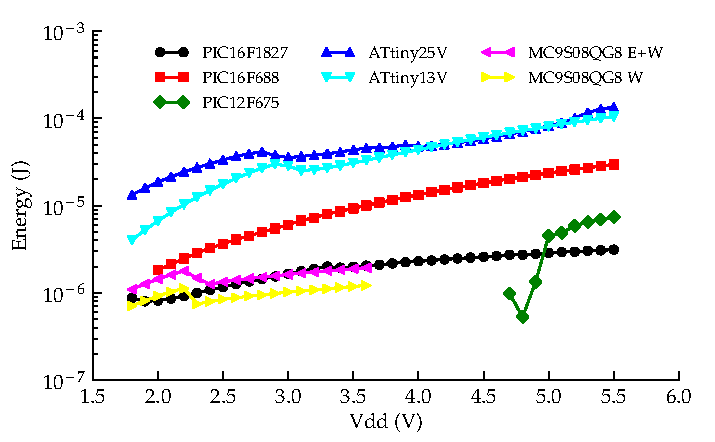
\includegraphics{content/pt1/03-EnergyRequirements/graphics/Graph_All_EEPROM_JPO}
        \caption{\label{fig:Energy-consumed-EEPROM}Graph showing energy consumed per non-volatile erase/write operation versus MCU supply voltage.}
      \end{figure}

      The energy consumption of each of the chips with EEPROM memory during a 1-byte write operation is shown as \cref{fig:Energy-consumed-EEPROM}.
      A curious situation arose with the PIC12F675 where its calculated energy consumption was negative when operated below \SI{4.7}{\volt}.
      It consumed \emph{less} current while performing write operations than running through the same code loop without performing writes.
      The measurement was repeated several times and produced the same result.
      Those data points were excluded from the plot as they do not represent the true energy cost of writing to EEPROM.
      It is likely that while writing to EEPROM other parts of this chip are disabled or put to sleep.

      In the case of the MC9S08QG8, which has Flash memory instead of EEPROM, the power consumption in the `E + W' trace was calculated as $1/512^{th}$ of consumed page erase energy consumption added to the energy cost of a single write operation.
      The trace labelled `W' (magenta) shows the energy cost for a single write operation.
      In order for the MC9S08QG8 to perform a write operation, the destination byte must have already been pre-erased at an earlier point in time.
      This may be useful for power harvesting since the energy expensive page erase operation, which consumes an average of \SI{302}{\micro\joule}, can be performed when available energy is plentiful.
      These results show that the Microchip and Freescale microprocessors are the most energy efficient when writing to non-volatile memory.



    \subsubsection{Analog-to-digital conversion}

      The operation of an electronic water meter may require that analogue-to-digital conversions are made.
      Measuring the amount of energy consumed per conversion was done in much the same way as the previous tests.
      Each of the chips had similar converters feature-wise.
      Results form the measurements are presented as \cref{fig:Energy-consumed-ADC}.

      \begin{figure}
        \centering
        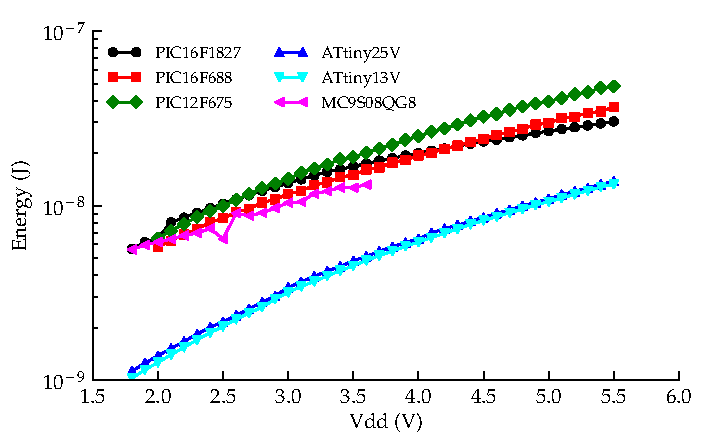
\includegraphics{content/pt1/03-EnergyRequirements/graphics/Graph_ALL_ADC_JPM}
        \caption{\label{fig:Energy-consumed-ADC}Graph showing the energy consumed per ADC measurement versus MCU supply voltage.}
      \end{figure}


  \section{Wireless Transmission}

    Because water meters are typically installed in remote areas where grid connection is unavailable, data must be collected via wireless interface.
    In Hamilton, a major utility provider has established a wireless mesh network between smart electricity meters installed in residential homes.
    That network utilises ZigBee wireless transceivers, making ZigBee an convenient choice for transmitting water metering data \cite{MalcolmSouness-WELNetworks2012}.
    Two types of wireless transmitters were chosen for energy measurement, a HOPE RF RFM12B transceiver and a Digi International Xbee Series 2 transceiver.
    The power consumption versus time during a wake, send one hundred and sixty bytes, and power down cycle was captured for both transceivers.
    By integrating the area under this curve the total energy consumed per transmission is found.
    The transmitters were kept \SI{1}{\meter} from there receivers with no obstructions between them.
    This represents ideal transmission conditions, something that our electronic water meter is very unlikely to encounter.
    The actual RF reception between a base station and installed meter will vary greatly between installations and weather conditions.
    For example, wet ground is likely to obstruct RF transmission due to the transmitter being shielded by a more conductive medium.
    Instead of trying to quantify the energy required in those situations, the best case was measured and an estimate of the worst case is estimated to be one hundred times larger.
    The transmit power can increase by a factor of 320 for the RFM module, however the transmit power only represents a proportion of total power usage.
    The modules must power up, start their internal oscillators, receive the data to be transmitted from the main processor and then transmit the data packets.
    I have crudely estimated that the difference between the lowest and the highest total power consumption, based on reception alone, will be a factor of 100.

    \begin{figure}
      \centering
      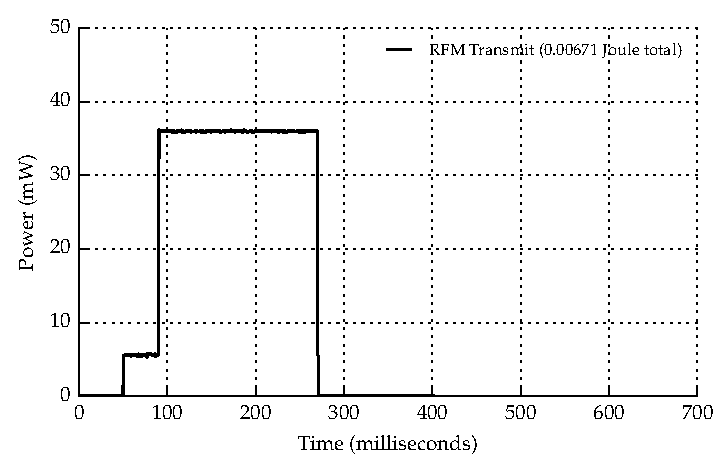
\includegraphics{content/pt1/03-EnergyRequirements/graphics/Graph_RFMPower.pdf}
      \caption{\label{fig:Energy-consumed-RFM12B}Graph of power draw from a HopeRF RFM12B transceiver module versus time during a power-up and transmit sequence.}
    \end{figure}

    \begin{figure}
      \centering
      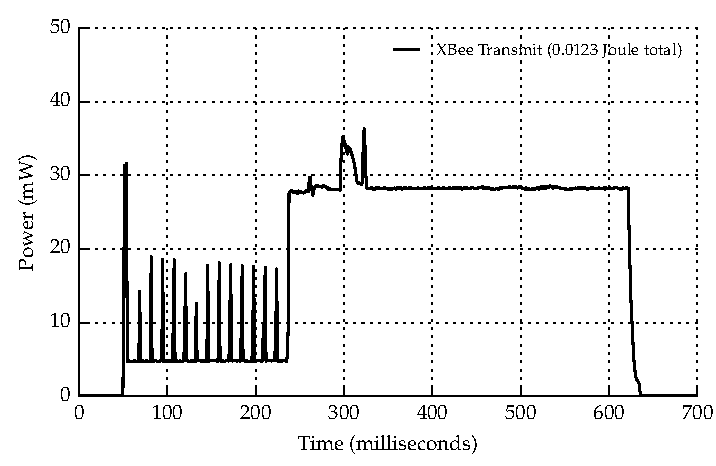
\includegraphics{content/pt1/03-EnergyRequirements/graphics/Graph_XbeePower.pdf}
      \caption{\label{fig:Energy-consumed-XBee}Graph of power draw from a Digi International Xbee Series 2 transceiver module versus time during a wake \& transmit sequence.}
    \end{figure}

    The RFM12B was operated at 433MHz, a frequency that is expected to increase the transmission through walls and soil.
    It has a maximum output power of \SI{5}{\decibel m} (\SI{3.2}{\milli\watt}) at this frequency.
    The Xbee has a maximum output power of \SI{0}{\decibel m} (\SI{1}{\milli\watt}) and operates at \SI{2.4}{\giga\hertz}.
    \Cref{fig:Energy-consumed-RFM12B,fig:Energy-consumed-XBee} show the captured power consumption during the tests.
    The RFM12B used about half as much energy sending the same data as the Xbee.
    Combined with its ability to operate at 433 MHz, the RFM12B is a sensible choice for the electronic water meter.
    In total the RFM consumed \SI{6.71}{\milli\joule} and the Xbee consumed \SI{12.3}{\milli\joule}.
    Adjusting these figures for the worst case (multiplying by one hundred) gives \SI{671}{\milli\joule} for the RFM12B and \SI{1.23}{\joule} for the Xbee.

  \section{Final Estimate of Energy Requirements}

    A crude estimation of an electronic water meter's microprocessor event loop is as follows.
    \begin{enumerate}
      \item Sleep for 1 second
      \item Execute 1000 instructions
      \item Make 2 analogue conversions
      \item Write 2 bytes to non-volatile memory
    \end{enumerate}
    This would allow the microprocessor to watch the display of a mechanical water meter and store the readings.
    This loop would occupy approximately one second, so it will occur 86400 times per day.
    Every so often the collected data would need to be transmitted, a potentially costly exercise in terms of energy usage.
    On top of the previously stated event loop is a data transmission loop which would execute every six hours.
    \begin{enumerate}
      \item Execute 1000000 instructions (Data compression)
      \item Power up and transmit 160 bytes of using RF transceiver
      \item Write 10 bytes to non-volatile memory
    \end{enumerate}

    \begin{table}
      \centering
      \begin{tabular}{|l|l|l|l|}
        \hline
        Mode & Count & Unit & Energy \\ \hline
        Sleep & 1 & seconds & \SI{97.4}{\nano\joule} \\
        Processing & 1000 & instructions & \SI{1.14}{\micro\joule} \\
        ADC & 2 & conversions & \SI{2.56}{\nano\joule} \\
        EEPROM & 2 & bytes & \SI{79.0}{\micro\joule} \\ \hline \hline
        &&Total (per day) & \SI{6.93}{\joule} \\ \hline
      \end{tabular}
      \caption{\label{tab:EnergyBudget-EventLoop} Estimated daily energy expenditure for basic processing functionality}
    \end{table}

    \begin{table}
      \centering
      \begin{tabular}{|l|l|l|l|}
        \hline
        Mode & Count & Unit & Energy \\ \hline
        Processing & 1000000 & instructions & \SI{1.14}{\milli\joule} \\
        Transmit & 160 & bytes & \SI{1.23}{\joule} \\
        EEPROM & 10 & bytes & \SI{394}{\micro\joule} \\ \hline \hline
        &&Total (per day) & \SI{4.93}{\joule} \\ \hline
      \end{tabular}
      \caption{\label{tab:EnergyBudget-Transmission}Estimated daily energy expenditure required to transmit 160 characters every six hours}
    \end{table}

    \Cref{tab:EnergyBudget-EventLoop,tab:EnergyBudget-Transmission} combine the measurements and estimates form the previous sections with the event loop estimation.
    They show that approximately \SI{12}{\joule} would be consumed per day by an electronic water meter.
    It was shown in \cref{sect:part1-WirelessWaterMeter-QuantifyingHarvestableEnergy} that \SI{280}{\joule} of energy is already dissipated in a mechanical water meter per day.
    This equates to a conversion efficiency of \SI{4.28}{\percent}, which would be the minimum efficiency required to run the meter continuously.

    % Edit checkpoint 2015-09-17 19:35

    %\section{Microcontrollers}
        %%!TEX root = ../../../thesis.tex

Harvesting power directly from flowing water opens the possibility of low-maintenance smart metering.


At the heart of a smart metering system is the microcontroller (MCU),
which among other things will be keeping track of the amount of water
consumed. In order to know whether it is possible to extract enough
power from a domestic water supply it is necessary to assess how much
power is required to run a microprocessor and any associated hardware.

In this chapter I compare power consumption and operational efficiencies
of six low power MCUs deemed suitable for running a power harvesting
water meter. The microprocessors to be investigated are low power,
general purpose 8-bit MCUs from three mainstream manufacturers, Microchip,
Atmel and Freescale. Measurement of power consumption will be carried
out during processing, sleeping and whilst undertaking two tasks that
are essential for smart water metering, analog-to-digital conversion
and non-volatile writes to memory.


\subsection{Selection of appropriate controllers}

The following microprocessors have been chosen as they represent a
well spaced selection from the three mainstream MCU manufacturers.
\begin{itemize}
\item Microchip PIC16F1827
\item Microchip PIC16F688
\item Microchip PIC12F675
\item Atmel ATtiny25V
\item Atmel ATtiny13V
\item Freescale MC9S08QG8
\end{itemize}
A basic feature comparison of the MCU selection is shown in table
%\ref{tab:MCUfeaturecomparison}.

\begin{sidewaystable}
\begin{centering}
\begin{tabular}{|l|l|l|l|l|l|l|l|}
\cline{2-8}
\multicolumn{1}{l|}{} & PIC16F1827  & PIC16F887  & PIC16F688  & PIC12F675  & ATtiny25V  & ATtiny13V  & MC9S08QG8 \tabularnewline
\hline
Vdd (min)  & 1.8  & 2.0  & 2.0V  & 2.0  & 1.8  & 1.8  & 1.8 \tabularnewline
Vdd (max)  & 5.5  & 5.5  & 5.5V  & 5.5  & 5.5  & 5.5  & 3.6 \tabularnewline
I (sleep)  & 30nA  & 50nA  & 50nA  & 1nA  & 100nA & <100nA & 450nA\tabularnewline
CLOCK (min)  & 31kHz  & 31kHz & 31kHz & 31kHz & 16kHz & 16kHz & 1MHz \tabularnewline
CLOCK (max)  & 32MHz  & 8MHz  & 8MHz  & 4MHz  & 16MHz & 9MHz  & 10MHz\tabularnewline
EEPROM  & 256B  & 256B  & 256B  & 128B  & 128B  & 64B  & \dag{}\tabularnewline
Serial  & USI  & USI  & USI  & --  & USI  & --  & USI \tabularnewline
USART  & UART  & UART  & UART  & --  & --  & --  & -- \tabularnewline
ADC  & 10bit  & 10bit & 10it  & 10bit & 10bit & 10bit & 10bit\tabularnewline
\hline
\end{tabular}
\par\end{centering}

\begin{centering}
\dag Has 8,192 bytes of software programmable flash (16 pages of 512
bytes each).
\par\end{centering}

\begin{centering}
\ddag Has 256 bytes of software programmable flash (4 pages of 64
bytes each).
\par\end{centering}

\centering{}\protect\caption{\label{tab:MCUfeaturecomparison} Feature comparison of selected MCUs.}
\end{sidewaystable}



% \section{Power consumption}

% Each of the MCUs were programmed to carry out various tasks which
% were performed over their specified range of operating voltages and
% operating frequencies. While the chips where carrying out these tasks
% their power consumption was measured by an Agilent E5270B Precision
% Mainframe via a PC and a Tektronix MSO 4054 Oscilloscope for timing
% purposes. Details on how each of the tests where carried out, as well
% as raw data, can be found in appendix %\ref{Appendix:Measurements} .


\subsection{Power consumption benchmarks}

Where possible the chips were configured to have each of their pins
set to outputs, held high, whilst being tied to Vdd via 10k$\Omega$
resistors. All chips had their peripherals disabled (where appropriate)
including any watchdog timers and brownout detection circuitry.

To allow more accurate sleep current measurements, the chips were
placed in a chip carrier with 10k$\Omega$ resistors soldered between
the pins (except ground and Vdd) and Vdd. They chip and carrier was
then washed in isopropyl alcohol and dried before being suspended
by connections to the the E5270. These steps were taken to reduce
any current leakage between pins due to fingerprints or dirt.


\subsection{Sleeping}

\begin{figure}
\begin{centering}
\includegraphics{content/pt1/02-Microcontrollers/graphics/Graph_All_Sleeping_Current}
\par\end{centering}

\centering{}\protect\caption{\label{fig:All_Sleep_Current}Current consumed by investigated MCUs
while in sleep mode.}
\end{figure}


A microprocessor in sleep mode is basically switched off, the only
difference being that volatile data is preserved provided the input
voltage doesn't fall below a minimum threshold voltage. In order to
consume as little power as possible an MCU should spend as much time
in sleep mode as is feasible. Power consumption during sleep therefore
plays a significant role in a chips ability to conserve power over
time.

\prettyref{fig:All_Sleep_Current} shows the amount of current consumed
by each of the MCUs while in their sleep state, note the log scale
on the y-axis. It can be seen that the PIC16F1827 consumes the most
current. This is somewhat contradictory to its specified sleep current
of 30nA \cite{PIC16F1827} (the second lowest of the set) at almost
1000 times higher. The Freescale MC9S08QG8 consumed energy at an average
of 11\% higher than specified \cite{MC9S08QG8}. Both the Atmel ATtiny13V
and ATtiny25V fell within their specification, \cite{AtmelATtiny13}
and \cite{AtmelATtiny25} respectively. There appears to be a trade-off
made between the two chips in the way of minimum power consumption
and minimum response to Vdd. The ATtiny13V required approximately
2.7 times less power than the ATtiny25V at 1.8V, but this advantage
rapidly falls away as Vdd moves up from 1.8V (and negated after 2.5V
Vdd). The Microchip PIC12F675 fell within specification\cite{PIC12F675}
and was the clear winner of the tested MCUs.

As the PIC16F1827 was so far off its specified value, the measurement
was repeated numerous times using code written in both assembler and
HI-TECH C as well as trying five different chips. All steps in the
datasheet to reduce power consumption where followed and all configuration
options where set, however no improvement was made.


\subsection{Processing}

Measuring the amount of power it takes to process information is not
a simple task. The way each chip carries out processing operations
internally can be quite different from one another, even though they
all produce the same result. This section will focus on the the energy
consumed while processing data and executing code.


\subsubsection*{Behind the scenes \label{sub:Behind-the-scenes}}

\begin{table}
\begin{centering}
\begin{tabular}{|c|c|}
\cline{2-2}
\multicolumn{1}{c|}{} & Instructions\tabularnewline
\hline
PIC16F1827 & 53\tabularnewline
\hline
PIC16F688 & 35\tabularnewline
\hline
PIC12F675 & 35\tabularnewline
\hline
ATtiny25V & 120\tabularnewline
\hline
ATtiny13V & 120\tabularnewline
\hline
MC9S08QG8 & 145\tabularnewline
\hline
\end{tabular}
\par\end{centering}

\centering{}\protect\caption{\label{tab:Number-of-instructions}Instruction set size for each tested
MCU.}
\end{table}


Not all MCUs are created equal, however this doesn't mean that some
are simply ``better'' than others. There are many complex factors
that determine the suitability of a particular MCU for a specific
task, one of which is the ability to crunch numbers. This section
is intended to give some background in plain-english of the relevant
inner workings that affect computational performance.

\begin{algorithm}[H]
\begin{lstlisting}
if (danger >= 5) flight();
else flee();
\end{lstlisting}
\protect\caption{\label{alg:Simple-C-code-representation}Simple C-code representation
of a branch instruction.}
\end{algorithm}


Algorithm \ref{alg:Simple-C-code-representation} shows a simplified
portion of C-code to demonstrate (very simply) how it may be implemented
in various ways. To determine whether or not the outcome of the code
is to fight or flee, the processor must first evaluate whether or
not the variable `danger' is greater than or equal to five and either
branch to the function `flight' or continue on to execute the function
`flee'.

\begin{algorithm}
\begin{lstlisting}
load 5 into register 001
load danger into register 002
branch-if-greater-or-equal 001 002 flee_call
call-subroutine fight
jump-to continue
[flee_call]
call-subroutine flee
[continue]
\end{lstlisting}
\protect\caption{\label{alg:Psudo-machine-code1}Psudo machine-code representation
of a branch instruction.}
\end{algorithm}





\begin{algorithm}
\begin{lstlisting}
load danger into register 001
subtract-from-register 001 5
branch-if-minus 001 fight_call
call-subroutine flee
jump-to continue
[fight_call]
call-subroutine fight
[continue]
\end{lstlisting}
\caption{\label{alg:Psudo-machine-code2}Psudo machine-code representation
of an alternative branch instruction.}
\end{algorithm}


Algorithms \ref{alg:Psudo-machine-code1} and \ref{alg:Psudo-machine-code2}
demonstrate two slightly different ways of implementing \ref{alg:Simple-C-code-representation}
in pseudo machine-code. The decision of which is best is made by the
compiler, which should take the instructional efficiency of the specific
MCU into account. This is an overly simplistic example, but its main
point is to illustrate that there are multiple paths that lead to
the same result. The important thing to note is that not all of those
paths require the same amount of effort. This means that the compiler's
ability to optimise code efficiently plays a role in determining the
overall performance of the chip. This also means that the programmer
shouldn't need to worry too much about instructional efficiency as
the compiler should transform C-code into machine code that best suits
the target MCU.

Another factor in processing efficiency comes down to the number of
different things (or instructions) it can do. All instructions for
each MCU are defined in its instruction set. Most 8-bit MCUs are based
on reduced instruction set computing (RISC) architecture, as opposed
to complex instruction set computing (CISC). This means that when
compared CISC based CPU, a RISC based chip is simpler and therefore
usually cheaper to produce. ``Instruction traces from CISC machines
consistently show that few of the available instructions are used
in most computing environments''\cite{ComputerArch}, meaning that
a lot of the added complexity in CISC designs is mostly underutilised.
To prevent confusion, a processor with a small instruction set can
perform all the same calculations that a processor with a larger instruction
set can so they are no less capable in a calculation sense. What this
means is that the processor with the reduced instruction set may need
to execute multiple instructions in order to achieve the same result
as an instruction from another processor which it doesn't have.

The final thing to note when comparing performance is that the clock
frequency of an MCU isn't necessarily the frequency at which it performs
operations, although sometimes it is.


\subsubsection*{Power consumed while processing}

\begin{figure}
\begin{centering}
\includegraphics{content/pt1/02-Microcontrollers/graphics/Graph_PIC16F1827_Clock_Power}
\par\end{centering}

\protect\caption{\label{graph:CLK_POWER_16F1827}Power consumed by the PIC16F1827 while
processing}
\end{figure}
\begin{figure}
\begin{centering}
\includegraphics{content/pt1/02-Microcontrollers/graphics/Graph_PIC16F688_Clock_Power}
\par\end{centering}

\protect\caption{\label{graph:CLK_POWER_16F688}Power consumed by the PIC16F688 while
processing}
\end{figure}
\begin{figure}
\begin{centering}
\includegraphics{content/pt1/02-Microcontrollers/graphics/Graph_PIC12F675_Clock_Power}
\par\end{centering}

\protect\caption{\label{graph:CLK_POWER_12F675-1}Power consumed by the PIC12F675 while
processing}
\end{figure}
\begin{figure}
\begin{centering}
\includegraphics{content/pt1/02-Microcontrollers/graphics/Graph_ATtiny25V_Clock_Power}
\par\end{centering}

\protect\caption{\label{graph:CLK_POWER_ATtiny25V}Power consumed by the ATtiny25V
while processing}
\end{figure}
\begin{figure}
\begin{centering}
\includegraphics{content/pt1/02-Microcontrollers/graphics/Graph_ATtiny13V_Clock_Power}
\par\end{centering}

\protect\caption{\label{graph:CLK_POWER_ATtiny13V}Power consumed by the ATtiny13V
while processing}
\end{figure}
\begin{figure}
\begin{centering}
\includegraphics{content/pt1/02-Microcontrollers/graphics/Graph_MC9S08QG8_Clock_Power}
\par\end{centering}

\protect\caption{\label{graph:CLK_POWER_MC9S08QG8}Power consumed by the MC9S08QG8
while processing}
\end{figure}


The Microchip PIC16F1827 displayed the lowest energy usage with 10$\mu A$
while clocking 7.75kIPS (as shown in figure \ref{graph:CLK_POWER_16F1827}).
It should be noted that the Microchip MCUs complete one instruction
cycle for every four clock cycles, so the 7.75kIPS corresponds to
a clock frequency of 31kHz. Also, not all instructions take one instruction
cycle to complete (as discussed in section \ref{sub:Behind-the-scenes}).
Figure \ref{graph:CLK_POWER_16F688} shows that the PIC16F688 consumes
less power than the PIC16F1827 while at low voltages for the same
instruction rates (except at 7.75kIPS). However, there appears to
be a flatter response in power consumption with respect to Vdd in
the PIC16F1827, similar to what was seen in figure \ref{fig:All_Sleep_Current}
with the Atmel chips.The PIC12F675 (as shown in \ref{graph:CLK_POWER_16F688})
used the same at the PIC16F688 (figure \ref{graph:CLK_POWER_16F688})
for its 1MIPS trace. Figures \ref{graph:CLK_POWER_ATtiny25V} and
\ref{graph:CLK_POWER_ATtiny13V} show both Atmel MCUs having similar
power requirements.The MC9S08QG8, although being able to clock the
slowest, performed very poorly at low frequencies. At 1.95kIPS it
consumed approximately the same amount of power as the Microchip MCUs
operating at 1MIPS.


\subsubsection*{Joules of energy consumed per instruction cycle\label{sub:Joules-of-energy}}

A convenient, and more insightful way to interpret the previous processing
power consumption graphs is to calculate the energy spent per instruction
performed. The energy cost of an instruction cycle can be calculated
using equation \ref{eq:JPI calculation}.

\begin{equation}
J_{i}=\frac{I\times Vdd}{f_{i}}\label{eq:JPI calculation}
\end{equation}
where $J_{i}$ is the number of joules consumed per instruction, $I$
is the current draw, $Vdd$ is the input voltage and $f_{i}$ is the
instruction frequency.

Figure \ref{fig:Per-instruction-cycle} compares the most energy efficient
operating conditions of each of the tested chips. What is most interesting
about this graph is amount of overlap between each of the chips. Also,
these greater efficiencies occur at high operating frequencies. A
simple rule of thumb for selecting the most power efficient operating
frequency based on these results is to choose the highest frequency
where the MCU can operate over its full input voltage (Vdd) range.
For comparison, figure \ref{fig:Per-instruction-ATtiny13V} shows
the trade-off made when selecting a higher frequency, which is typical
across the range of MCUs tested.

\begin{figure}
\begin{centering}
\includegraphics{content/pt1/02-Microcontrollers/graphics/Graph_All_Clock_JPI}
\par\end{centering}

\protect\caption{\label{fig:Per-instruction-cycle}Per instruction cycle energy consumption
comparison}
\end{figure}
\begin{figure}
\begin{centering}
\includegraphics{content/pt1/02-Microcontrollers/graphics/Graph_ATtiny13V_Clock_JPI}
\par\end{centering}

\protect\caption{\label{fig:Per-instruction-ATtiny13V}Per instruction cycle energy
consumption of the ATtiny13V}
\end{figure}



\subsubsection*{Performance benchmark}

In section \ref{sub:Joules-of-energy} I presented a graph showing
the amount of energy consumed per instruction cycle for each MCU under
ideal operating conditions. But, as discussed in section \ref{sub:Behind-the-scenes},
not all instructions take one instruction cycle to complete. Also,
some MCUs have extra instructions that are designed to help speed-up
code execution by combining commonly used pairs of instructions. This
section will look at how many instruction cycles each MCU takes to
complete a benchmarking function. Which will allow a more accurate
representation of execution efficiency to be made.

For the benchmarking function I wanted something that would consume
a large number of instructions cycles, be well suited to an 8-bit
microcontroller (i.g. no complex maths functions and small memory
footprint) and have a well defined end point. For this I chose a linear
feedback shift register based pseudo-random number generator (as shown
in \ref{alg:Benchmarking-algorithm}), for which the code was sourced
from \cite{LinearFeedbackRegister}.

In short, this function starts with a 16-bit number and runs it through
the linear feedback register in a tight loop until the initial value
of the 16-bit feedback register is produced again. This function steps
through every possible combination of bits possible in a 16-bit number
(except zero; 65535) in a pseudo-random order before exiting the loop.
The function combines the exclusive-OR (XOR), bit shifting, bitwise
AND, increment a value and numerical comparison operations in a tight
loop.

\begin{algorithm}
\begin{lstlisting}
unsigned short lfsr = 0xACE1u;
unsigned period = 0;
do {
	lfsr = (lfsr >> 1) ^ (-(lfsr & 1u) & 0xB400u);
	++period;
} while(lfsr != 0xACE1u);
\end{lstlisting}
\caption{\label{alg:Benchmarking-algorithm}Benchmarking algorithm}
\end{algorithm}


The benchmarking function was compiled and run on each of the MCUs
operating at a range of frequencies. The amount of time each MCU took
to complete the benchmark was timed by watching a pin that toggled
on completion of the benchmark function with a Tektronix MSO 4054
Oscilloscope. The number of instruction cycles each chip took to complete
the benchmark was deduced by multiplying the time taken to complete
the benchmark by the instruction cycle frequency. The results of the
benchmark are shown in figure \ref{fig:GraphBar_All_Benchmark}. It
should be noted that to calculate the number of instruction cycles
taken by the Microchip family of processors (PIC16F1827, PIC16F688
and PIC12F675) the chip frequency divided by four was used, meaning
that the number of clock cycles consumed was four times higher. It
is clear from figure \ref{fig:GraphBar_All_Benchmark} that the Atmel
(ATtiny25V and ATtiny13V) microprocessors are by far the most efficient
microprocessor in terms of executing code using a minimum number of
instructions of the selection.

\begin{figure}
    \begin{centering}
        \includegraphics{content/pt1/02-Microcontrollers/graphics/Graph_All_Clock_Benchmark}
    \end{centering}
    \protect\caption{\label{fig:GraphBar_All_Benchmark}MCU comparison of instructions
    taken to complete a benchmark.}
\end{figure}



\subsection{Non-volatile memory}

In order for a microprocessor to keep information about its current
state and recorded data in the event of power loss it must write to
non-volatile memory. Non-volatile memory is implemented as either
electrically erasable and programmable read only memory (EEPROM) or
Flash memory. Flash memory is similar to EEPROM with the exception
that it must be erased in large blocks, or pages, before it can be
written to. All of the tested MCUs have on-board EEPROM with the exception
of the MC9S08QG8 which has flash memory instead. Table \ref{tab:MCUfeaturecomparison}
shows the amount of non-volatile memory space available on each of
the chips. The energy consumption of each of the chips with EEPROM
memory during a 1-byte write operation (which also includes a 1-byte
erase operation) is shown in figure \ref{fig:Energy-consumed-EEPROM}.
There appears to be a glitch with the PIC12F675 with respect to it's
energy consumption. It's energy consumption was calculated as negative
with a Vdd below 4.7V, meaning that it consumed less current while
performing write operations than running through the same program
loop without performing writes. The measurement was repeated several
times and produced the same result but I did not further pursue the
cause. I have concluded that this is not representative of the MCU
and have disregarded EEPROM measurement data for this chip. In the
case of the MC9S08QG8, which has Flash memory instead of EEPROM, the
power consumption in the E + W case was calculated per erase/write
operation to be $1/512^{th}$ of the page erase energy consumption
added to the energy cost of a single write operation, where the W
case was the energy cost of a single write operation. In order for
the MC9S08QG8 to perform a write operation, the destination byte must
have already been pre-erased at an earlier point in time. This may
be useful for power harvesting since the energy expensive page erase
operation, which consumes an average of 3.02e-4 Joules, can be done
performed when available energy is plentiful.

\begin{figure}
\begin{centering}
\includegraphics{content/pt1/02-Microcontrollers/graphics/Graph_All_EEPROM_JPO}
\par\end{centering}

\protect\caption{Energy consumed by each MCU per non-volatile erase/write operation.\label{fig:Energy-consumed-EEPROM}}
\end{figure}



\subsection{Analog-to-digital conversions.}

To measure the flow of water the chosen MCU will likely either count
pulses record a voltage level from a flow meter. It is possible that
another mechanism such as ultrasonic flow measurement may be used
but for now only analog-to-digital (ADC) measurements will be measured.
For those unfamiliar with an ADC, it is simply a way of converting
a voltage (which is generally free to change) into a digital number
that a MCU can process and/or store. The power consumption per ADC
measurement for each of the tested MCUs is shown in figure \ref{fig:Energy-consumed-ADC}.

\begin{figure}
\begin{centering}
\includegraphics{content/pt1/02-Microcontrollers/graphics/Graph_ALL_ADC_JPM}
\protect\caption{Energy consumed by each MCU per ADC measurement.\label{fig:Energy-consumed-ADC}}

\par\end{centering}

\end{figure}



    %\section{Data Transmission}
        %
\section{Power Consumption}

\begin{figure}
\begin{centering}
\protect\caption{Power consumption of ZigBee}

\par\end{centering}

\end{figure}
\begin{figure}

\begin{centering}
\protect\caption{Power consumption of RFM12B}

\par\end{centering}

\end{figure}



  \chapter{Discussion}
  \label{chap:part_1_discussion}

  \chapter{Conclusion}
  \label{chap:part_1_conclusion}


%% Part 3 - Double layers on conductors
\part{Double Layers on Conductors: Electrical Impedance}
  \label{part:doubleLayersOnConductors}
  \chapter{Introduction}
    \section{Background}
    \section{Literature Review}

  \chapter{An Interfacial Model In The Electrical Domain}
    %!TEX root = ../../thesis.tex

\section{The Scott-Single Interface Model}
  \subsection{Solution resistivity}
  \subsection{Constant phase element}
  \subsection{Faradaic current}
  \subsection{Species depletion}
\section{Methods of Parameter Extraction}
  \subsection{Resistivity and constant phase element}
  \subsection{Faradaic currents}



  \chapter{Extraction of Interface Model Parameters}
    %!TEX root = ../../thesis.tex

\section{Phosphate Buffered Saline}
    \subsection{Resistivity and constant phase element}
    \subsection{Faradaic current}

        Faradaic processes at an electrode/electrolyte interface are modeled
        by the Butler-Volmer equation:

        \begin{equation}
        i_{net}=i_{o}\left\{ \frac{[O]_{(0,t)}}{[O]_{\infty}}e^{\frac{-\alpha_{c}nF\eta}{RT}}-\frac{[R]_{(0,t)}}{[R]_{\infty}}e^{\frac{(1-\alpha_{c})nF\eta}{RT}}\right\}
        \end{equation}


        where:

        \begin{tabular}{rl}
        $i_{net}$ & = net Faradaic current\tabularnewline
        $i_{o}$ & = current exchange density\tabularnewline
        $[O]_{(0,t)}$ & = concentration of oxidising species at electrode surface $(x=0)$\tabularnewline
        $[R]_{(0,t)}$ & = concentration of reducing species at the electrode surface\tabularnewline
        $[O]_{\infty}$ & = bulk concentration of oxidising species in electrolyte\tabularnewline
        $[R]_{\infty}$ & = bulk concentration of oxidising species in electrolyte\tabularnewline
        $\alpha_{c}$ & = cathodic transfer coefficient\tabularnewline
        $n$ & = number of moles of electrons per mole of reactant oxidised\tabularnewline
        F & = Faraday's constant $\approx96,485$\tabularnewline
        R & = the gas constant $\approx8.314$\tabularnewline
        T & = absolute temperature in Kelvin\tabularnewline
        $\eta$ & = electrode overpontential\tabularnewline
        \end{tabular}


    \subsection{Discussion}

\section{Biological parameter measurements}
    \label{sect:sheep_measurements}
    \subsection{Resistivity and constant phase element}
    \subsection{Discussion}


  \chapter{Recipes For Fluid Mimicry}
  \label{chap:fluid_mimicry}
    %!TEX root = ../../thesis.tex

Utilising the measurement methods used previously, I search for a liquid that better replicates a biological impedance.
This work is of benefit to engineers of medical implant devices.
Having the ability to formulate a solution that mimics the electrical conditions inside a living being greatly simplifies testing.

It was discovered through collaboration with Saluda Medical, developers of stimulator implants, that a solution of one-tenth the standard solution of phosphate buffered saline is used as a test fluid.
This solution was the best substitute for a living spine that the engineers had.
It was held in large buckets in the laboratories for use whenever a quick test needed to be carried out.
Electrodes are submerged into these buckets in order to recreate the electrical conditions inside a human spine.

This was not the only way to simulate the impedance conditions inside a person.
As presented in~\cref{sect:sheep_measurements}, the use of anaesthetised sheep were also used.
A sheep's spine has roughly the same dimensions as a humans so it represents a sensible choice in terms of geometry.
However, the resources involved with conducting a live sheep trial were high; requiring use of a hospital operating theatre, surgeon veterinarian, and equipment.

Engineers at Saluda had no way of knowing how well those baths of saline represented a sheep's spine.
It was shown in \cref{sect:sheep_measurements} that the match between the two was weak.
With that knowledge, and the measurement techniques developed thus far, we now ask if it is possible to create a better match.
Such a match would reduce the number of surgical operations the test engineers might need to conduct, saving resources.


\section{Measurements}

This work is a very recent addition to the previous work at the time of writing.
The measurements were not conducted in a laboratory environment, so it is expected that some inaccuracies will exist.
These inaccuracies will be related to:
\begin{enumerate}
    \item a lack of temperature control, meaning temperatures fluctuated between 18 and 26 degrees;
    \item use of consumer grade scales, jeweller's scales for under 5 grams and kitchen above;
    \item use of consumer grade ingredients and distilled water.
\end{enumerate}
The measurement equipment used to conduct the measurements were the same as those used in the lab.

\subsection{Configuration}

The function generator, Agilent 33220A, and oscilloscope, Tektronix TPS 2024, are connected to the electrode array, St. Jude Medical - Octrode, as is shown in \cref{fig:creatingCSF_setup}.
A \SI{10}{\kilo\ohm} resistor was used to measure the current driven between electrodes eight and three.
It had a measured resistance of \SI{9.990}{\kilo\ohm}, as measured with a Fluke Digital Multimeter.

\begin{figure}
    \centering
    \includegraphics[scale=0.95]{content/pt2/graphics/CreatingCSF_setup}
    \caption{\label{fig:creatingCSF_setup}Diagram showing the measurement configuration used to measure the CPE response and resistivity of mixed solutions}
\end{figure}

\subsection{Procedure}

Each measurement run begin at the upper end of the frequency spectrum and proceeded towards the low frequency endpoint.
Starting with the higher frequencies offers a chance to confirm correct measurement set-up early in the measurement.
A sample at the lowest frequency can take over a minute to acquire, where the higher frequencies drop to under a second.
The same frequencies were chosen that were used to measure the situation in live sheep.
This allows easy comparison between the sheep data and the impedance of mixed solutions.

Measurements were completely automated via a Linux based computer running Python scripts.
These scripts controlled the output settings of the waveform generator and acquired the resulting waveforms from the oscilloscope.
The scripts had the ability to set the horizontal and vertical scales on the oscilloscope channels in order to ensure appropriate scales were used.
These scripts were written by myself and have been made freely available through my github account (\url{https://github.com/MarkHedleyJones/pyLabInstruments})

\begin{figure}
    \centering
    \includegraphics[width=\textwidth]{content/pt2/graphics/measurementFlowchart}
    \caption{\label{fig:creatingCSF_pythonFlowchart}Diagram showing the execution of the measurement script}
\end{figure}

The measurement procedure followed by the script is shown as a simplified flowchart in \cref{fig:creatingCSF_pythonFlowchart}.
The programme steps through each of the required frequencies, making sure the target voltage is developed across electrodes seven and eight, calculating the interface impedance.

The target voltage across the interface is \SI{20}{\milli\volt}.
This voltage was previously determined as a safe stimulus voltage in that it does not trigger Faradaic reactions at the electrode's surface.
Because the impedance of the interface changes with frequency, it is necessary to alter the output amplitude to keep the voltage across electrode seven and eight consistent.

This measurement configuration differs from the three channel method used in earlier measurements.
Those used channel three of the oscilloscope to watch the voltage developed between electrodes three and eight.

\subsection{Ingredients Tried}
To determine how certain additives affect the impedance of the interface, a wide range of ingredients were mixed and tested.
They were used in a semi-random order, chosen to maximise the usage of the quantity of distilled water available at the time.
\begin{itemize}
    \item Glycerol
    \item Methylated Spirits
    \item Sodium Carbonate
    \item Sodium Bicarbonate
    \item Table-salt (non-iodised)
    \item Gelatine
    \item Citric Acid
    \item Corn-flour
\end{itemize}

\subsection{Results}

\subsubsection*{Water, Corn-flour and Salt}

\begin{figure}
    \centering
    \includegraphics[width=\textwidth]{content/pt2/graphics/run12_600ml-distilledWater_ZVsF_graph_mag}
    \caption{\label{fig:recipe_water_mag}Plot of impedance magnitude versus frequency (log-log) for distilled water.}
\end{figure}

\begin{figure}
    \centering
    \includegraphics[width=\textwidth]{content/pt2/graphics/run12_600ml-distilledWater_ZVsF_graph_phase}
    \caption{\label{fig:recipe_water_phase}Plot of impedance phase versus frequency (log-log) for distilled water.}
\end{figure}

\begin{figure}
    \centering
    \includegraphics[width=\textwidth]{content/pt2/graphics/run14_170ml-distilledWater_250g-cornflour_ZVsF_graph_mag}
    \caption{\label{fig:recipe_cornflour_mag}Plot of impedance magnitude versus frequency (log-log) for \SI{250}{\gram} cornflour mixed with \SI{175}{\milli\litre} distilled water.}
\end{figure}

\begin{figure}
    \centering
    \includegraphics[width=\textwidth]{content/pt2/graphics/run14_170ml-distilledWater_250g-cornflour_ZVsF_graph_phase}
    \caption{\label{fig:recipe_cornflour_phase}Plot of impedance phase versus frequency (log-log) for \SI{250}{\gram} cornflour mixed with \SI{175}{\milli\litre} distilled water.}
\end{figure}

\begin{figure}
    \centering
    \includegraphics[width=\textwidth]{content/pt2/graphics/run14_175ml-distilledWater_250g-cornflour_1g9-salt_ZVsF_graph_mag}
    \caption{\label{fig:recipe_cornflour_salt_mag}Plot of impedance magnitude versus frequency (log-log) for \SI{250}{\gram} cornflour mixed with \SI{175}{\milli\litre} distilled water and \SI{1.9}{\gram} table-salt.}
\end{figure}

\begin{figure}
    \centering
    \includegraphics[width=\textwidth]{content/pt2/graphics/run14_175ml-distilledWater_250g-cornflour_1g9-salt_ZVsF_graph_phase}
    \caption{\label{fig:recipe_cornflour_salt_phase}Plot of impedance phase versus frequency (log-log) for \SI{250}{\gram} cornflour mixed with \SI{175}{\milli\litre} distilled water and \SI{1.9}{\gram} table-salt.}
\end{figure}

\begin{figure}
    \centering
    \includegraphics[width=\textwidth]{content/pt2/graphics/run14_180ml-distilledWater_250g-cornflour_1g9-salt_ZVsF_graph_mag}
    \caption{\label{fig:recipe_cornflour_salt_extraWater_mag}Plot of impedance magnitude versus frequency (log-log) for \SI{250}{\gram} cornflour mixed with \SI{180}{\milli\litre} distilled water and \SI{1.9}{\gram} table-salt.}
\end{figure}

\begin{figure}
    \centering
    \includegraphics[width=\textwidth]{content/pt2/graphics/run14_180ml-distilledWater_250g-cornflour_1g9-salt_ZVsF_graph_phase}
    \caption{\label{fig:recipe_cornflour_salt_extraWater_phase}Plot of impedance phase versus frequency (log-log) for \SI{250}{\gram} cornflour mixed with \SI{180}{\milli\litre} distilled water and \SI{1.9}{\gram} table-salt.}
\end{figure}

\Cref{fig:recipe_water_mag,fig:recipe_water_phase,fig:recipe_cornflour_phase,fig:recipe_cornflour_mag,fig:recipe_cornflour_phase,fig:recipe_cornflour_salt_mag,fig:recipe_cornflour_salt_phase,fig:recipe_cornflour_salt_extraWater_mag,fig:recipe_cornflour_salt_extraWater_phase} show a progression of measurements beginning with distilled water, then adding cornflour, then adding salt, and finally adding a very small amount of extra water.

\subsubsection*{Improved Water, Corn-flour, and Salt}

\begin{figure}
    \centering
    \includegraphics[width=\textwidth]{content/pt2/graphics/run12_190ml-distilledWater_190g-cornflour_0g858-salt_ZVsF_graph_mag}
    \caption{\label{fig:recipe_cornflour_salt_extraWater_mag_improved}Plot of impedance magnitude versus frequency (log-log) for \SI{190}{\gram} cornflour mixed with \SI{190}{\milli\litre} distilled water and \SI{0.858}{\gram} table-salt.}
\end{figure}

\begin{figure}
    \centering
    \includegraphics[width=\textwidth]{content/pt2/graphics/run12_190ml-distilledWater_190g-cornflour_0g858-salt_ZVsF_graph_phase}
    \caption{\label{fig:recipe_cornflour_salt_extraWater_phase_improved}Plot of impedance phase versus frequency (log-log) for \SI{190}{\gram} cornflour mixed with \SI{190}{\milli\litre} distilled water and \SI{0.858}{\gram} table-salt.}
\end{figure}

\Cref{fig:recipe_cornflour_salt_extraWater_mag_improved,fig:recipe_cornflour_salt_extraWater_phase_improved} show the results of mixing the same set of ingredients as the previous measurement set, but with the closest fit to sheep spine obtained.


\subsection{Discussion}

These results show that it is possible to alter the CPE response and the bulk conductivity of the solution independently of one another.

Each of the measurements that contained salt had a tendency to ``fall-over'' at low frequency.
The salt


%% Part 4 - Appendices
\part{Appendices}
  \appendix
  \chapter{Charged Droplet Energy Harvester}
    \label{appendix:chargedDropletts}
    %!TEX root = ../../../thesis.tex
\begin{figure}
    \centering
    \includegraphics[width=0.5\textwidth]{content/appendices/chargedWaterDrops/graphics/Figure_Drawing_KelvinWaterDripper_OriginalDevice}
    \caption{Drawing of Lord Kelvin's electrostatic generator~\cite{Thomson1867a}.}
    \label{Figure_Drawing_KelvinWaterDripper_OriginalDevice}
\end{figure}
In 1867 William Thomson (Lord Kelvin) described an apparatus that could generate electrostatic charge using drops of water~\cite{Thomson1867}.
\Cref{Figure_Drawing_KelvinWaterDripper_OriginalDevice} shows original artwork of the device from that paper.
It works by inducing charge onto drops of water before they detach from the source of the drips.
This device was the starting point of investigation into the use of charged water drops to generate electrical power.


\section{Generating Charge}

  \begin{figure}
      \centering
      \includegraphics[height=0.25\textheight]{content/appendices/chargedWaterDrops/graphics/Figure_Drawing_KelvinWaterDripper_ChargingMechanism}
      \caption{Drawing of the charging mechanism for Lord Kelvin's electrostatic
  generator}
      \label{Figure_Drawing_KelvinWaterDripper_ChargingMechanism}
  \end{figure}
  Figure \ref{Figure_Drawing_KelvinWaterDripper_ChargingMechanism} shows charge generating mechanism of Lord Kelvin's electrostatic generator.
  This mechanism is comprised of three main components:
  \begin{enumerate}
  \item a jet of water which breaks into droplets,
  \item an inducting ring surrounding the area where the jet breaks up,
  \item a receiver where the charged droplets are collected.
  \end{enumerate}
  \begin{figure}
      \centering
      \includegraphics{content/appendices/chargedWaterDrops/graphics/DripperOut}
      \caption{\label{Fig_Diagram_KelvinWaterDripper}Simplified diagram of Lord Kelvin's water dropper configuration}
  \end{figure}
  A diagram showing a variation of that design with both sides present is shown as \cref{Fig_Diagram_KelvinWaterDripper}.
  The polarity of each receiver and induction ring is represented by its colour.
  Equal and opposite charge is accumulated in the receivers below the nozzles.
  The receivers are electrically isolated from each other, but are connected to the induction rings of the opposite side.
  The induction rings push charge away from the drop as it forms on the positive side, and pulls charge onto drops forming on the negative side.
  Gravity then pulls the drops down into the receivers below.
  Because the receiver and the drip both have the same polarity electric field, they repel each other.
  The drop, because of gravity and the height it falls from, is doing work as it falls into the receiver as the integral of the electrostatic force over the distance it travels.
  The result of that work is an increase in static charge held by the receiver, measured as voltage.


\section{Optimising output}

  Summer research student Jonathon McMullen assembled a test-rig to recreate the experiment.
  Once constructed, another summer research student, Wayne Crump, and myself took measurements.
  Then we sought to optimise the design in the hopes that is may be suitable as an energy harvester.


  \subsection*{Drop volume and frequency}

    The first optimisation question was ``is it better to have many small or fewer but larger drops?''.
    A simplified experiment was made with the help of Wayne Crump.
    We aimed to remove as many variables from the experiment that was previously performed by Jonathan McMullen.
    By doing so we hoped to isolate the effect of varying drop size, induction voltage, and flow rate, had on output power.


  \subsubsection*{Experimental setup}

  \begin{figure}[ht]
        \centering
        \includegraphics[scale=0.15]{content/appendices/chargedWaterDrops/graphics/Photo_dripperExperiment_Setup_draft.JPG}
        \caption{\label{Photo_dripperExperiment_Setup}Photo of experimental setup for charge on drip measurements.}
    \end{figure}

    \begin{figure}[ht]
        \centering
        \includegraphics[scale=0.9]{content/appendices/chargedWaterDrops/graphics/ChargedDrips_Figure_Drawing_ExperimentalSetup}
        \caption{\label{ChargedDrips_Figure_Drawing_ExperimentalSetup}Diagram of experimental setup for charge on drip experiments.}
    \end{figure}

    \begin{figure}[ht]
        \centering
        \includegraphics[scale=0.12]{content/appendices/chargedWaterDrops/graphics/Photo_dripperExperiment_Inductor_draft.JPG}
        \caption{Photo of the dropper and high voltage inductor.}
        \label{Photo_dripperExperiment_Inductor}
    \end{figure}

    \begin{figure}[ht]
        \centering
        \includegraphics[scale=0.15]{content/appendices/chargedWaterDrops/graphics/Photo_dripperExperiment_SyringePump_draft.JPG}
        \caption{\label{Photo_dripperExperiment_SyringePump}Photo of the syringe pump used to produce drops and control flow rate.}
    \end{figure}

    A photo of the measurement setup is shown in \cref{Photo_dripperExperiment_Setup}.
    A simplified diagram of that same setup is shown in \cref{ChargedDrips_Figure_Drawing_ExperimentalSetup}.
    Drips are formed from a syringe needle which then fall through the induction ring before hitting the tin foil.
    A close-up of photo of the needle and inductor is shown in \cref{Photo_dripperExperiment_Inductor}.
    The drips frequency is determined by a microphone paced under the foil and the flow of water is set by the syringe pump (shown in \cref{Photo_dripperExperiment_SyringePump}).
    The volume of each drip is calculated by dividing the flow rate by the drip frequency.
    The charge on each drop is determined by dividing the average current through the multimeter by the drip frequency.
    Measured current was in the nano Ampere range so direct current measurement with a multimeter was not possible.
    Instead, the multimeter was set to measure voltage and the internal resistance of the meter itself was used as the current sense resistor.
    The multimeter had an internal resistance of \SI{10}{\mega\ohm}.
%    Ohms law states:
%    \begin{equation}
%    V=IR
%    \end{equation}
%    Where V is voltage, I is current and R is resistance.
%    Rearranging this equation and substituting in our resistance of \SI{10}{\mega\ohm} gives:
%
%    \begin{equation}
%    I=\frac{V}{10\times10^{6}}
%    \end{equation}
%    Where V is the output of the multimeter and I is the current through
%    the multimeter, through which we assume all charge collected on the
%    tin foil will flow.

  \subsubsection*{Results}

    \begin{figure}
        \centering
        \includegraphics{content/appendices/chargedWaterDrops/graphics/dripper_chargeVsVolume}
        \caption{\label{Graph_dripperExperiment_chargeVsVolume}Charge on drip versus drip volume for a fixed induction voltage of \SI{2.5}{\kilo\volt}.}
    \end{figure}
    \begin{figure}
        \centering
        \includegraphics{content/appendices/chargedWaterDrops/graphics/dripper_chargePerVolumeVsVolume}
        \caption{\label{Figure_Graph_dripper_chargePerVolumeVsVolume}Charge per volume
        versus drop volume for a fixed induction voltage of \SI{2.5}{\kilo\volt}.}
    \end{figure}
    \begin{figure}
        \includegraphics{content/appendices/chargedWaterDrops/graphics/dripper_chargeVsVoltage}
        \caption{\label{Figure_Graph_dripper_chargeVsVoltage}Graph showing charge on a drop versus induction voltage for a fixed drop volume.}
    \end{figure}
    Figure \ref{Figure_Graph_dripper_currentVsFlow} shows the effect of increasing the flow on the output current; a relatively linear response.
    \begin{figure}
        \centering
        \includegraphics{content/appendices/chargedWaterDrops/graphics/dripper_currentVsFlow}
        \caption{\label{Figure_Graph_dripper_currentVsFlow}Graph showing current versus flow rate for an induction voltage of \SI{3.8}{\kilo\volt} and drop volume of \SI{3.1}{\micro\litre}.}
    \end{figure}
    Figure \ref{Graph_dripperExperiment_chargeVsVolume} shows the effect of drip volume on the bound charge per drop.
    This curve resembles the surface area of a sphere against the volume of a sphere.
    This was expected as excess charge will distribute itself over the outer surface of the drop, and therefore be proportional to its surface area.
    If the same data is plotted in terms of charge per volume versus volume of a drip, as is shown in Figure \ref{Figure_Graph_dripper_chargePerVolumeVsVolume}, it is evident that smaller drop sizes equate to a higher charge per volume of water ratio.
    Figure \ref{Figure_Graph_dripper_chargeVsVoltage} shows the results of changing the induction voltage on the average charge carried per drop.
    The results show the charge induced on a drop is proportional to the induction voltage.
    Variation in the measurement data is due to variations in room temperature.


  \subsubsection*{Conclusion \& discussion}

    Increasing the output of the generator is possible by:
    \begin{itemize}
    \item reducing the drop size for a given volumetric flow rate,
    \item increasing the volumetric flow rate,
    \item increasing the voltage on the induction ring.
    \end{itemize}
    Increasing the volumetric flow through a nozzle causes drops to turn into a stream above a flow threshold.
    If that stream does not break into drops before connecting with the receiving vessel then charge held in the vessel can travel up the stream; short-circuiting the device.
    If the stream does reliably break into droplets then the induction ring should be positioned as close to the transition point as possible.
    Reducing drop size and increasing the induction voltage both increase the charge to mass ratio of individual drops.
    As this ratio increases, the movement of drops becomes increasingly dominated by the electrostatic force between the receiver and the drop.
    The force repels the drop from the receiver meaning that the drops start to bend away from the receiver as they fall.
    Increasing the charge-to-mass ratio too far cause drops to escape the receiver.
    It is possible with a sufficiently large charge-to-mass ratio for the water droplets path to bend back upward to the induction ring, i.e., the water ``falls upwards'' back to the high voltage ring.
    A nozzle capable of producing consistent drop volumes allows for the greatest efficiency since the charge per drop can be maximised with the least reduction of drop catchment.

  \subsection*{Scale}

    Lord Kelvin's original design of electrostatic generator is too big to fit inside a water meter.
    Because of its size the voltage differential required to create the target electrostatic field strength is large; approximately \SI{4}{\kilo\volt}.
    A reduction in physical size would lower this voltage while keeping the electric field gradient the same.
    Notice in \cref{Photo_dripperExperiment_Inductor} how revolved cuts have been made in the arm supporting the induction ring to increase electrical isolation.
    Lower voltages would mean less electrical isolation is necessary keep the device from self-discharging.
    Reducing the scale of the device would allow it to generate a maximum output at voltages that are easier to process using conventional electronics.


%  \subsubsection*{Investigation:}
%
%    \begin{figure}
%        \centering
%        \includegraphics{content/appendices/chargedWaterDrops/graphics/ChargedDrips_Figure_Diagram_Forces}
%        \caption{\label{Figure_Diagram_ChargedDrips_Figure_Diagram_Forces}Diagram
%    of the electrostatic force and gravity acting on a drop of water.}
%    \end{figure}
%
%
%    Figure \ref{Figure_Diagram_ChargedDrips_Figure_Diagram_Forces} shows
%    a simplified diagram of the two dominant forces acting upon a charged
%    drop as it falls towards a like charged plate from a grounded plane.
%    These forces are given by the following equations:
%    \begin{equation}
%    F_{down}=mg
%    \end{equation}
%    \begin{equation}
%    F_{up}=qE
%    \end{equation}
%    where $m$ is the mass of the drop, $g$ is the acceleration due to
%    gravity, $q$ is the charge on the drop and $E$ is the electric field
%    strength.

  \chapter{Microprocessor Power Measurements}
    %!TEX root = ../../../thesis.tex

\label{Appendix:Measurements}


\section{Measurement scripts}

Energy consumption measurements were made using an Agilent E5270B
8-Slot Precision Measurement Mainframe, a Tektronix MSO 4054 Mixed
Signal Oscilloscope and a desktop PC. Operation of the E5270 was done
via GLIB interface using a USB connection and Agilent IO Libraries
Version 16.0.1458.0. From here the machine was interfaced using custom
Python scripts (appended) and PyVisa (available from \url{http://pyvisa.sourceforge.net/pyvisa/} ).

\subsection{E5270 Scripts}

Measurement of chip energy consumption was carried out using the following
measurement script. This script is written in Python and was executed
using PyLab from the Enthought Python bundle.

\verbatiminput{content/appendices/microprocessorPowerMeasurements/Microcontrollers/measDev.py}


\section{Measurement data}

It should be noted that the Freescale M9S08QG8 and the Microchip PIC16F1827
were unable to boot reliably into a low power state at 1.8V. To prevent
this from happening the chips were booted at 2.0V and lowered to 1.8V
to prevent the chips entering a state where current consumption was
in the hundreds of microamps range.


\subsection{Chips sleeping}

The following tables list the unprocessed current measurements for
a sweep of Vdd from 1.8V to 5.5V. Sweeps have been restricted to the
input voltage ranges as specified in each chips datasheet.

\begin{table}[htp]
\begin{centering}
\begin{tabular}{|r|r|r|r|r|r|}
\hline
Vdd  & Tiny13V  & Tiny25V  & 12F675  & 16F1827  & M9S08QG8\tabularnewline
\hline
1.80  & 3.41E-08  & 9.27E-08  & N/A  & 9.914E-07  & 3.82E-04 \tabularnewline
1.90  & 4.04E-08  & 9.30E-08  & N/A  & 1.008E-06  & 3.86E-04 \tabularnewline
2.00  & 4.73E-08  & 9.33E-08  & 4.497E-10  & 1.023E-06  & 4.88E-07 \tabularnewline
2.10  & 5.47E-08  & 9.36E-08  & 4.677E-10  & 1.038E-06  & 4.89E-07 \tabularnewline
2.20  & 6.26E-08  & 9.39E-08  & 4.797E-10  & 1.054E-06  & 4.91E-07 \tabularnewline
2.30  & 7.10E-08  & 9.42E-08  & 4.907E-10  & 1.068E-06  & 4.92E-07 \tabularnewline
2.40  & 7.99E-08  & 9.45E-08  & 5.057E-10  & 1.087E-06  & 4.94E-07 \tabularnewline
2.50  & 8.92E-08  & 9.47E-08  & 5.210E-10  & 1.102E-06  & 4.96E-07 \tabularnewline
2.60  & 9.90E-08  & 9.50E-08  & 5.347E-10  & 1.119E-06  & 4.99E-07 \tabularnewline
2.70  & 1.09E-07  & 9.53E-08  & 5.487E-10  & 1.137E-06  & 5.02E-07 \tabularnewline
2.80  & 1.20E-07  & 9.56E-08  & 5.610E-10  & 1.166E-06  & 5.05E-07 \tabularnewline
2.90  & 1.31E-07  & 9.59E-08  & 5.760E-10  & 1.195E-06  & 5.10E-07 \tabularnewline
3.00  & 1.42E-07  & 9.63E-08  & 5.903E-10  & 1.234E-06  & 5.15E-07 \tabularnewline
3.10  & 1.54E-07  & 9.66E-08  & 6.057E-10  & 1.290E-06  & 5.21E-07 \tabularnewline
3.20  & 1.67E-07  & 9.70E-08  & 6.217E-10  & 1.300E-06  & 5.28E-07 \tabularnewline
3.30  & 1.79E-07  & 9.74E-08  & 6.397E-10  & 1.301E-06  & 5.37E-07 \tabularnewline
3.40  & 1.92E-07  & 9.78E-08  & 6.590E-10  & 1.302E-06  & 5.47E-07 \tabularnewline
3.50  & 2.06E-07  & 9.82E-08  & 6.763E-10  & 1.301E-06  & 5.60E-07 \tabularnewline
3.60  & 2.20E-07  & 9.87E-08  & 6.970E-10  & 1.304E-06  & 5.75E-07 \tabularnewline
3.70  & 2.35E-07  & 9.93E-08  & 7.200E-10  & 1.307E-06  & N/A \tabularnewline
3.80  & 2.49E-07  & 1.00E-07  & 7.437E-10  & 1.309E-06  & N/A \tabularnewline
3.90  & 2.65E-07  & 1.01E-07  & 7.703E-10  & 1.311E-06  & N/A \tabularnewline
4.00  & 2.80E-07  & 1.02E-07  & 7.960E-10  & 1.312E-06  & N/A \tabularnewline
4.10  & 2.97E-07  & 1.03E-07  & 8.273E-10  & 1.317E-06  & N/A \tabularnewline
4.20  & 3.13E-07  & 1.04E-07  & 8.690E-10  & 1.319E-06  & N/A \tabularnewline
4.30  & 3.31E-07  & 1.05E-07  & 9.033E-10  & 1.330E-06  & N/A \tabularnewline
4.40  & 3.48E-07  & 1.07E-07  & 9.487E-10  & 1.334E-06  & N/A \tabularnewline
4.50  & 3.67E-07  & 1.09E-07  & 9.977E-10  & 1.342E-06  & N/A \tabularnewline
4.60  & 3.86E-07  & 1.11E-07  & 1.056E-09  & 1.351E-06  & N/A \tabularnewline
4.70  & 4.05E-07  & 1.13E-07  & 1.117E-09  & 1.360E-06  & N/A \tabularnewline
4.80  & 4.25E-07  & 1.16E-07  & 1.197E-09  & 1.373E-06  & N/A \tabularnewline
4.90  & 4.46E-07  & 1.19E-07  & 1.296E-09  & 1.385E-06  & N/A \tabularnewline
5.00  & 4.67E-07  & 1.23E-07  & 1.403E-09  & 1.401E-06  & N/A \tabularnewline
5.10  & 4.90E-07  & 1.27E-07  & 1.513E-09  & 1.422E-06  & N/A \tabularnewline
5.20  & 5.13E-07  & 1.32E-07  & 1.661E-09  & 1.445E-06  & N/A \tabularnewline
5.30  & 5.37E-07  & 1.38E-07  & 1.811E-09  & 1.469E-06  & N/A \tabularnewline
5.40  & 5.62E-07  & 1.45E-07  & 1.975E-09  & 1.497E-06  & N/A \tabularnewline
5.50  & 5.88E-07  & 1.53E-07  & 2.164E-09  & 1.529E-06  & N/A \tabularnewline
\hline
\end{tabular}
\par\end{centering}

\protect\caption{Raw sleep measurements (Vdd 1.8V -- 5.5V)}
\end{table}
\begin{figure}
\begin{centering}
\includegraphics{content/appendices/microprocessorPowerMeasurements/graphics/Graph_All_Sleeping_Power}
\par\end{centering}

\protect\caption{\label{fig:All_SleepPower}Power usage of each microprocessor while
in sleep mode}


\end{figure}


Figure \ref{fig:All_Sleep_Current} shows the amount of current drawn
by each of the microprocessors in sleep mode. Similarly, figure \ref{fig:All_SleepPower}
shows the power consumption of each of the chips in sleep mode.


\subsection{Clocking}


\subsubsection*{ATtiny13V}

\begin{sidewaystable}
\begin{centering}
\begin{tabular}{|r|r|r|r|r|r|r|}
\hline
Vdd  & 9.6 MHz  & 4.8 MHz  & 1.2 MHz  & 600 kHz  & 128 kHz  & 16 kHz\tabularnewline
\hline
1.80  & N/A  & N/A  & 3.900E-04  & 2.148E-04  & 8.098E-05  & 5.393E-05 \tabularnewline
1.90  & N/A  & N/A  & 4.121E-04  & 2.258E-04  & 8.387E-05  & 5.499E-05 \tabularnewline
2.00  & N/A  & N/A  & 4.242E-04  & 2.329E-04  & 8.708E-05  & 5.608E-05 \tabularnewline
2.10  & N/A  & N/A  & 4.429E-04  & 2.421E-04  & 8.897E-05  & 5.721E-05 \tabularnewline
2.20  & N/A  & N/A  & 4.634E-04  & 2.523E-04  & 9.126E-05  & 5.839E-05 \tabularnewline
2.30  & N/A  & N/A  & 4.859E-04  & 2.632E-04  & 9.415E-05  & 5.964E-05 \tabularnewline
2.40  & N/A  & N/A  & 5.088E-04  & 2.748E-04  & 9.738E-05  & 6.099E-05 \tabularnewline
2.50  & N/A  & N/A  & 5.323E-04  & 2.865E-04  & 1.006E-04  & 6.214E-05 \tabularnewline
2.60  & N/A  & N/A  & 5.557E-04  & 2.984E-04  & 1.038E-04  & 6.396E-05 \tabularnewline
2.70  & 2.759E-03  & 1.664E-03  & 5.799E-04  & 3.108E-04  & 1.071E-04  & 6.560E-05 \tabularnewline
2.80  & 2.879E-03  & 1.742E-03  & 6.065E-04  & 3.235E-04  & 1.102E-04  & 6.743E-05 \tabularnewline
2.90  & 3.001E-03  & 1.834E-03  & 6.384E-04  & 3.366E-04  & 1.136E-04  & 6.926E-05 \tabularnewline
3.00  & 3.116E-03  & 1.945E-03  & 6.705E-04  & 3.540E-04  & 1.174E-04  & 7.100E-05 \tabularnewline
3.10  & 3.231E-03  & 2.022E-03  & 6.876E-04  & 3.582E-04  & 1.124E-04  & 6.809E-05 \tabularnewline
3.20  & 3.358E-03  & 2.109E-03  & 7.144E-04  & 3.710E-04  & 1.150E-04  & 6.878E-05 \tabularnewline
3.30  & 3.486E-03  & 2.199E-03  & 7.421E-04  & 3.843E-04  & 1.175E-04  & 6.996E-05 \tabularnewline
3.40  & 3.619E-03  & 2.295E-03  & 7.700E-04  & 3.979E-04  & 1.200E-04  & 7.115E-05 \tabularnewline
3.50  & 3.757E-03  & 2.394E-03  & 7.976E-04  & 4.114E-04  & 1.226E-04  & 7.235E-05 \tabularnewline
3.60  & 3.905E-03  & 2.491E-03  & 8.269E-04  & 4.251E-04  & 1.250E-04  & 7.354E-05 \tabularnewline
\hline
\end{tabular}
\par\end{centering}

\protect\caption{Atmel ATtiny13V clocking current (Vdd 1.8V -- 3.6V).}


\end{sidewaystable}
\begin{sidewaystable}
\begin{centering}
\begin{tabular}{|r|r|r|r|r|r|r|}
\hline
Vdd  & 9.6 MHz  & 4.8 MHz  & 1.2 MHz  & 600 kHz  & 128 kHz  & 16 kHz\tabularnewline
\hline
3.70  & 4.046E-03  & 2.580E-03  & 8.555E-04  & 4.392E-04  & 1.275E-04  & 7.471E-05 \tabularnewline
3.80  & 4.185E-03  & 2.661E-03  & 8.854E-04  & 4.535E-04  & 1.298E-04  & 7.706E-05 \tabularnewline
3.90  & 4.322E-03  & 2.740E-03  & 9.156E-04  & 4.685E-04  & 1.321E-04  & 7.701E-05 \tabularnewline
4.00  & 4.464E-03  & 2.822E-03  & 9.467E-04  & 4.834E-04  & 1.343E-04  & 7.814E-05 \tabularnewline
4.10  & 4.606E-03  & 2.900E-03  & 9.780E-04  & 4.990E-04  & 1.365E-04  & 7.929E-05 \tabularnewline
4.20  & 4.753E-03  & 2.932E-03  & 1.010E-03  & 5.152E-04  & 1.386E-04  & 8.045E-05 \tabularnewline
4.30  & 4.901E-03  & 2.991E-03  & 1.043E-03  & 5.313E-04  & 1.406E-04  & 8.163E-05 \tabularnewline
4.40  & 5.061E-03  & 3.001E-03  & 1.077E-03  & 5.491E-04  & 1.425E-04  & 8.283E-05 \tabularnewline
4.50  & 5.219E-03  & 2.987E-03  & 1.110E-03  & 5.655E-04  & 1.444E-04  & 8.406E-05 \tabularnewline
4.60  & 5.389E-03  & 3.073E-03  & 1.144E-03  & 5.833E-04  & 1.462E-04  & 8.531E-05 \tabularnewline
4.70  & 5.547E-03  & 3.162E-03  & 1.178E-03  & 6.002E-04  & 1.480E-04  & 8.661E-05 \tabularnewline
4.80  & 5.710E-03  & 3.257E-03  & 1.213E-03  & 6.216E-04  & 1.498E-04  & 8.795E-05 \tabularnewline
4.90  & 5.872E-03  & 3.348E-03  & 1.248E-03  & 6.395E-04  & 1.502E-04  & 8.932E-05 \tabularnewline
5.00  & 6.046E-03  & 3.443E-03  & 1.285E-03  & 6.567E-04  & 1.484E-04  & 9.072E-05 \tabularnewline
5.10  & 6.228E-03  & 3.548E-03  & 1.320E-03  & 6.746E-04  & 1.470E-04  & 9.213E-05 \tabularnewline
5.20  & 6.391E-03  & 3.647E-03  & 1.357E-03  & 6.940E-04  & 1.465E-04  & 9.346E-05 \tabularnewline
5.30  & 6.575E-03  & 3.753E-03  & 1.394E-03  & 7.134E-04  & 1.469E-04  & 9.482E-05 \tabularnewline
5.40  & 6.753E-03  & 3.857E-03  & 1.434E-03  & 7.331E-04  & 1.485E-04  & 9.640E-05 \tabularnewline
5.50  & 6.955E-03  & 3.970E-03  & 1.471E-03  & 7.526E-04  & 1.506E-04  & 9.818E-05 \tabularnewline
\hline
\end{tabular}
\par\end{centering}

\protect\caption{Atmel ATtiny13V clocking current (Vdd 3.7V -- 5.5V).}


\end{sidewaystable}
\begin{figure}
\begin{centering}
\includegraphics{content/appendices/microprocessorPowerMeasurements/graphics/Graph_ATtiny13V_Clock_Current}
\par\end{centering}

\protect\caption{
\label{fig:ATtiny13VClkCurrent}Current consumption of the Atmel ATtiny13V
while clocking
}


\end{figure}
\begin{figure}
\begin{centering}
\includegraphics{content/appendices/microprocessorPowerMeasurements/graphics/Graph_ATtiny13V_Clock_Power}
\par\end{centering}

\protect\caption{
\label{fig:ATtiny13VClkPower}Power consumption of the Atmel ATtiny13V
while clocking
}
\end{figure}
\begin{figure}
\begin{centering}
\includegraphics{content/appendices/microprocessorPowerMeasurements/graphics/Graph_ATtiny13V_Clock_JPI}
\par\end{centering}

\protect\caption{
\label{fig:ATtiny13VClkJPI}Energy consumed per instruction for the
Atmel ATtiny13V
}


\end{figure}



\subsubsection*{ATtiny25V}

\begin{sidewaystable}
\begin{centering}
\begin{tabular}{|r|r|r|r|r|r|r|r|r|}
\hline
Vdd  & 16 MHz  & 8 MHz  & 6.4 MHz  & 2 MHz  & 1 MHz  & 800 kHz  & 128 kHz  & 16 kHz \tabularnewline
\hline
1.80  & N/A  & N/A  & N/A  & 1.148E-03  & 4.106E-04  & 1.146E-03  & 7.622E-05  & 1.666E-04 \tabularnewline
1.90  & N/A  & N/A  & N/A  & 1.205E-03  & 4.319E-04  & 1.209E-03  & 7.858E-05  & 1.737E-04 \tabularnewline
2.00  & N/A  & N/A  & N/A  & 1.261E-03  & 4.531E-04  & 1.274E-03  & 8.121E-05  & 1.813E-04 \tabularnewline
2.10  & N/A  & N/A  & N/A  & 1.320E-03  & 4.754E-04  & 1.339E-03  & 8.464E-05  & 1.903E-04 \tabularnewline
2.20  & N/A  & N/A  & N/A  & 1.378E-03  & 4.984E-04  & 1.404E-03  & 8.981E-05  & 1.994E-04 \tabularnewline
2.30  & N/A  & N/A  & N/A  & 1.434E-03  & 5.195E-04  & 1.471E-03  & 9.486E-05  & 2.066E-04 \tabularnewline
2.40  & N/A  & N/A  & N/A  & 1.491E-03  & 5.413E-04  & 1.537E-03  & 9.642E-05  & 2.126E-04 \tabularnewline
2.50  & N/A  & N/A  & N/A  & 1.540E-03  & 5.671E-04  & 1.604E-03  & 9.903E-05  & 2.193E-04 \tabularnewline
2.60  & N/A  & N/A  & N/A  & 1.597E-03  & 5.912E-04  & 1.671E-03  & 1.008E-04  & 2.257E-04 \tabularnewline
2.70  & 6.283E-03  & 3.124E-03  & 1.765E-03  & 1.651E-03  & 6.163E-04  & 1.740E-03  & 1.030E-04  & 2.320E-04 \tabularnewline
2.80  & 6.551E-03  & 3.256E-03  & 1.842E-03  & 1.706E-03  & 6.425E-04  & 1.811E-03  & 1.053E-04  & 2.378E-04 \tabularnewline
2.90  & 6.826E-03  & 3.392E-03  & 1.916E-03  & 1.766E-03  & 6.683E-04  & 1.883E-03  & 1.072E-04  & 2.414E-04 \tabularnewline
3.00  & 7.097E-03  & 3.537E-03  & 1.995E-03  & 1.832E-03  & 6.963E-04  & 1.959E-03  & 1.094E-04  & 2.434E-04 \tabularnewline
3.10  & 7.380E-03  & 3.682E-03  & 2.081E-03  & 1.906E-03  & 7.284E-04  & 2.050E-03  & 1.118E-04  & 2.440E-04 \tabularnewline
3.20  & 7.695E-03  & 3.825E-03  & 2.172E-03  & 1.973E-03  & 7.623E-04  & 2.131E-03  & 1.143E-04  & 2.469E-04 \tabularnewline
3.30  & 7.996E-03  & 3.975E-03  & 2.253E-03  & 2.036E-03  & 7.925E-04  & 2.210E-03  & 1.170E-04  & 2.521E-04 \tabularnewline
3.40  & 8.288E-03  & 4.122E-03  & 2.340E-03  & 2.101E-03  & 8.216E-04  & 2.286E-03  & 1.190E-04  & 2.587E-04 \tabularnewline
3.50  & 8.605E-03  & 4.271E-03  & 2.425E-03  & 2.165E-03  & 8.516E-04  & 2.371E-03  & 1.208E-04  & 2.657E-04 \tabularnewline
3.60  & 8.915E-03  & 4.421E-03  & 2.510E-03  & 2.230E-03  & 8.824E-04  & 2.452E-03  & 1.222E-04  & 2.732E-04 \tabularnewline
\hline
\end{tabular}
\par\end{centering}

\protect\caption{Atmel ATtiny25V clocking current (Vdd 3.7V -- 5.5V)}


\end{sidewaystable}
\begin{sidewaystable}
\begin{centering}
\begin{tabular}{|r|r|r|r|r|r|r|r|r|}
\hline
Vdd  & 16 MHz  & 8 MHz  & 6.4 MHz  & 2 MHz  & 1 MHz  & 800 kHz  & 128 kHz  & 16 kHz \tabularnewline
\hline
3.70  & 9.232E-03  & 4.582E-03  & 2.599E-03  & 2.298E-03  & 9.122E-04  & 2.535E-03  & 1.235E-04  & 2.805E-04 \tabularnewline
3.80  & 9.550E-03  & 4.754E-03  & 2.687E-03  & 2.365E-03  & 9.436E-04  & 2.622E-03  & 1.246E-04  & 2.867E-04 \tabularnewline
3.90  & 9.908E-03  & 4.921E-03  & 2.776E-03  & 2.436E-03  & 9.746E-04  & 2.706E-03  & 1.258E-04  & 2.950E-04 \tabularnewline
4.00  & 1.025E-02  & 5.077E-03  & 2.864E-03  & 2.506E-03  & 1.006E-03  & 2.795E-03  & 1.269E-04  & 2.951E-04 \tabularnewline
4.10  & 1.057E-02  & 5.245E-03  & 2.962E-03  & 2.578E-03  & 1.040E-03  & 2.882E-03  & 1.280E-04  & 3.015E-04 \tabularnewline
4.20  & 1.092E-02  & 5.422E-03  & 3.054E-03  & 2.652E-03  & 1.074E-03  & 2.970E-03  & 1.278E-04  & 3.085E-04 \tabularnewline
4.30  & 1.128E-02  & 5.607E-03  & 3.153E-03  & 2.724E-03  & 1.108E-03  & 3.062E-03  & 1.279E-04  & 3.159E-04 \tabularnewline
4.40  & 1.161E-02  & 5.783E-03  & 3.250E-03  & 2.795E-03  & 1.143E-03  & 3.155E-03  & 1.270E-04  & 3.235E-04 \tabularnewline
4.50  & 1.198E-02  & 5.958E-03  & 3.348E-03  & 2.873E-03  & 1.177E-03  & 3.248E-03  & 1.266E-04  & 3.313E-04 \tabularnewline
4.60  & 1.235E-02  & 6.139E-03  & 3.445E-03  & 2.949E-03  & 1.210E-03  & 3.340E-03  & 1.254E-04  & 3.390E-04 \tabularnewline
4.70  & 1.272E-02  & 6.312E-03  & 3.549E-03  & 3.027E-03  & 1.248E-03  & 3.430E-03  & 1.240E-04  & 3.468E-04 \tabularnewline
4.80  & 1.311E-02  & 6.501E-03  & 3.653E-03  & 3.105E-03  & 1.284E-03  & 3.528E-03  & 1.230E-04  & 3.547E-04 \tabularnewline
4.90  & 1.349E-02  & 6.689E-03  & 3.757E-03  & 3.190E-03  & 1.319E-03  & 3.633E-03  & 1.229E-04  & 3.625E-04 \tabularnewline
5.00  & 1.387E-02  & 6.898E-03  & 3.860E-03  & 3.270E-03  & 1.358E-03  & 3.732E-03  & 1.237E-04  & 3.703E-04 \tabularnewline
5.10  & 1.427E-02  & 7.099E-03  & 3.965E-03  & 3.356E-03  & 1.396E-03  & 3.832E-03  & 1.248E-04  & 3.781E-04 \tabularnewline
5.20  & 1.464E-02  & 7.302E-03  & 4.075E-03  & 3.437E-03  & 1.432E-03  & 3.931E-03  & 1.262E-04  & 3.857E-04 \tabularnewline
5.30  & 1.506E-02  & 7.502E-03  & 4.181E-03  & 3.527E-03  & 1.471E-03  & 4.033E-03  & 1.277E-04  & 3.930E-04 \tabularnewline
5.40  & 1.547E-02  & 7.713E-03  & 4.297E-03  & 3.616E-03  & 1.512E-03  & 4.142E-03  & 1.293E-04  & 3.999E-04 \tabularnewline
5.50  & 1.588E-02  & 7.908E-03  & 4.415E-03  & 3.705E-03  & 1.552E-03  & 4.245E-03  & 1.311E-04  & 4.063E-04 \tabularnewline
\hline
\end{tabular}
\par\end{centering}

\protect\caption{Atmel ATtiny25V clocking current (VDD 3.7V -- 5.5V)}


\end{sidewaystable}
\begin{figure}
\begin{centering}
\includegraphics{content/appendices/microprocessorPowerMeasurements/graphics/Graph_ATtiny13V_Clock_Current}
\par\end{centering}

\protect\caption{\label{fig:ATtiny25VClkCurrent}Current consumption of the Atmel ATtiny25V
while clocking}


\end{figure}
\begin{figure}
\begin{centering}
\includegraphics{content/appendices/microprocessorPowerMeasurements/graphics/Graph_ATtiny25V_Clock_Power}
\par\end{centering}

\protect\caption{
\label{fig:ATtiny25VClkPower}Power consumption of the Atmel ATtiny25V
while clocking
}


\end{figure}
\begin{figure}
\begin{centering}
\includegraphics{content/appendices/microprocessorPowerMeasurements/graphics/Graph_ATtiny25V_Clock_JPI}
\par\end{centering}

\protect\caption{
\label{fig:ATtiny25VClkJPI}Energy consumed per instruction for the
Atmel ATtiny25V
}


\end{figure}



\subsubsection*{Microchip PIC16F1827}

\begin{sidewaystable}
\begin{centering}
\begin{tabular}{|r|r|r|r|r|r|r|r|r|}
\hline
Vdd  & 32 MHz  & 16 MHz  & 8 MHz  & 4 MHz  & 2 MHz  & 1 MHz  & 500 kHz  & 31 kHz \tabularnewline
\hline
1.80  & N/A  & 1.250E-03  & 8.043E-04  & 5.163E-04  & 3.912E-04  & 3.290E-04  & 1.327E-04  & 4.679E-06 \tabularnewline
1.90  & N/A  & 1.322E-03  & 8.483E-04  & 5.391E-04  & 4.066E-04  & 3.405E-04  & 1.367E-04  & 4.892E-06 \tabularnewline
2.00  & N/A  & 1.395E-03  & 8.930E-04  & 5.619E-04  & 4.220E-04  & 3.520E-04  & 1.402E-04  & 5.063E-06 \tabularnewline
2.10  & N/A  & 1.468E-03  & 9.382E-04  & 5.848E-04  & 4.375E-04  & 3.637E-04  & 1.436E-04  & 5.307E-06 \tabularnewline
2.20  & N/A  & 1.542E-03  & 9.841E-04  & 6.079E-04  & 4.528E-04  & 3.754E-04  & 1.471E-04  & 5.546E-06 \tabularnewline
2.30  & N/A  & 1.620E-03  & 1.031E-03  & 6.310E-04  & 4.683E-04  & 3.870E-04  & 1.503E-04  & 5.796E-06 \tabularnewline
2.40  & N/A  & 1.698E-03  & 1.078E-03  & 6.544E-04  & 4.838E-04  & 3.987E-04  & 1.535E-04  & 5.996E-06 \tabularnewline
2.50  & 2.711E-03  & 1.773E-03  & 1.126E-03  & 6.778E-04  & 4.996E-04  & 4.105E-04  & 1.567E-04  & 6.282E-06 \tabularnewline
2.60  & 2.826E-03  & 1.848E-03  & 1.172E-03  & 7.008E-04  & 5.150E-04  & 4.223E-04  & 1.599E-04  & 6.536E-06 \tabularnewline
2.70  & 2.939E-03  & 1.919E-03  & 1.214E-03  & 7.232E-04  & 5.301E-04  & 4.337E-04  & 1.631E-04  & 6.734E-06 \tabularnewline
2.80  & 3.050E-03  & 1.990E-03  & 1.255E-03  & 7.456E-04  & 5.450E-04  & 4.449E-04  & 1.662E-04  & 6.912E-06 \tabularnewline
2.90  & 3.163E-03  & 2.062E-03  & 1.297E-03  & 7.685E-04  & 5.605E-04  & 4.565E-04  & 1.695E-04  & 7.109E-06 \tabularnewline
3.00  & 3.277E-03  & 2.134E-03  & 1.338E-03  & 7.916E-04  & 5.758E-04  & 4.683E-04  & 1.728E-04  & 7.349E-06 \tabularnewline
3.10  & 3.391E-03  & 2.207E-03  & 1.380E-03  & 8.152E-04  & 5.917E-04  & 4.802E-04  & 1.763E-04  & 7.534E-06 \tabularnewline
3.20  & 3.507E-03  & 2.281E-03  & 1.422E-03  & 8.388E-04  & 6.074E-04  & 4.919E-04  & 1.797E-04  & 7.601E-06 \tabularnewline
3.30  & 3.623E-03  & 2.355E-03  & 1.465E-03  & 8.626E-04  & 6.235E-04  & 5.039E-04  & 1.829E-04  & 7.604E-06 \tabularnewline
3.40  & 3.445E-03  & 2.263E-03  & 1.438E-03  & 8.666E-04  & 6.386E-04  & 5.273E-04  & 1.940E-04  & 7.638E-06 \tabularnewline
3.50  & 3.445E-03  & 2.263E-03  & 1.439E-03  & 8.663E-04  & 6.390E-04  & 5.276E-04  & 1.942E-04  & 7.582E-06 \tabularnewline
3.60  & 3.447E-03  & 2.264E-03  & 1.439E-03  & 8.663E-04  & 6.389E-04  & 5.275E-04  & 1.943E-04  & 7.616E-06 \tabularnewline
\hline
\end{tabular}
\par\end{centering}

\protect\caption{Microchip PIC16F1827 clocking current (Vdd 0V -- 3.6V)}


\end{sidewaystable}
\begin{sidewaystable}
\begin{centering}
\begin{tabular}{|r|r|r|r|r|r|r|r|r|}
\hline
Vdd  & 32 MHz  & 16 MHz  & 8 MHz  & 4 MHz  & 2 MHz  & 1 MHz  & 500 kHz  & 31 kHz \tabularnewline
\hline
3.70  & 3.449E-03  & 2.265E-03  & 1.439E-03  & 8.663E-04  & 6.392E-04  & 5.277E-04  & 1.945E-04  & 7.617E-06 \tabularnewline
3.80  & 3.449E-03  & 2.265E-03  & 1.440E-03  & 8.665E-04  & 6.393E-04  & 5.279E-04  & 1.947E-04  & 7.649E-06 \tabularnewline
3.90  & 3.450E-03  & 2.265E-03  & 1.440E-03  & 8.667E-04  & 6.397E-04  & 5.283E-04  & 1.950E-04  & 7.603E-06 \tabularnewline
4.00  & 3.451E-03  & 2.267E-03  & 1.441E-03  & 8.669E-04  & 6.396E-04  & 5.283E-04  & 1.952E-04  & 7.634E-06 \tabularnewline
4.10  & 3.452E-03  & 2.267E-03  & 1.441E-03  & 8.672E-04  & 6.401E-04  & 5.286E-04  & 1.955E-04  & 7.633E-06 \tabularnewline
4.20  & 3.453E-03  & 2.268E-03  & 1.442E-03  & 8.673E-04  & 6.401E-04  & 5.286E-04  & 1.957E-04  & 7.667E-06 \tabularnewline
4.30  & 3.454E-03  & 2.269E-03  & 1.442E-03  & 8.675E-04  & 6.404E-04  & 5.290E-04  & 1.960E-04  & 7.620E-06 \tabularnewline
4.40  & 3.454E-03  & 2.269E-03  & 1.443E-03  & 8.679E-04  & 6.405E-04  & 5.293E-04  & 1.961E-04  & 7.660E-06 \tabularnewline
4.50  & 3.456E-03  & 2.270E-03  & 1.443E-03  & 8.681E-04  & 6.410E-04  & 5.294E-04  & 1.964E-04  & 7.663E-06 \tabularnewline
4.60  & 3.457E-03  & 2.271E-03  & 1.444E-03  & 8.684E-04  & 6.412E-04  & 5.297E-04  & 1.966E-04  & 7.704E-06 \tabularnewline
4.70  & 3.458E-03  & 2.271E-03  & 1.444E-03  & 8.687E-04  & 6.416E-04  & 5.300E-04  & 1.969E-04  & 7.664E-06 \tabularnewline
4.80  & 3.458E-03  & 2.272E-03  & 1.445E-03  & 8.690E-04  & 6.417E-04  & 5.303E-04  & 1.972E-04  & 7.710E-06 \tabularnewline
4.90  & 3.460E-03  & 2.273E-03  & 1.446E-03  & 8.692E-04  & 6.421E-04  & 5.307E-04  & 1.976E-04  & 7.721E-06 \tabularnewline
5.00  & 3.461E-03  & 2.274E-03  & 1.446E-03  & 8.695E-04  & 6.424E-04  & 5.310E-04  & 1.979E-04  & 7.757E-06 \tabularnewline
5.10  & 3.463E-03  & 2.275E-03  & 1.447E-03  & 8.697E-04  & 6.428E-04  & 5.314E-04  & 1.983E-04  & 7.733E-06 \tabularnewline
5.20  & 3.464E-03  & 2.276E-03  & 1.448E-03  & 8.699E-04  & 6.433E-04  & 5.319E-04  & 1.986E-04  & 7.762E-06 \tabularnewline
5.30  & 3.465E-03  & 2.277E-03  & 1.448E-03  & 8.703E-04  & 6.437E-04  & 5.326E-04  & 1.991E-04  & 7.797E-06 \tabularnewline
5.40  & 3.467E-03  & 2.278E-03  & 1.449E-03  & 8.708E-04  & 6.444E-04  & 5.332E-04  & 1.996E-04  & 7.777E-06 \tabularnewline
5.50  & 3.468E-03  & 2.279E-03  & 1.450E-03  & 8.711E-04  & 6.449E-04  & 5.336E-04  & 2.002E-04  & 7.833E-06 \tabularnewline
\hline
\end{tabular}
\par\end{centering}

\protect\caption{Microchip PIC16F1827 clocking current (Vdd 3.7V -- 5.5V)}
\end{sidewaystable}
\begin{figure}
\begin{centering}
\includegraphics{content/appendices/microprocessorPowerMeasurements/graphics/Graph_PIC16F1827_Clock_Current}
\par\end{centering}

\protect\caption{\label{fig:16F1827ClkCurrent}Current consumption of the Microchip
PIC16F1827 while clocking}


\end{figure}
\begin{figure}
\begin{centering}
\includegraphics{content/appendices/microprocessorPowerMeasurements/graphics/Graph_PIC16F1827_Clock_Power}
\par\end{centering}

\protect\caption{
\label{fig:16F1827ClkPower}Power consumption of the Microchip PIC16F1827
while clocking
}


\end{figure}
\begin{figure}
\begin{centering}
\includegraphics{content/appendices/microprocessorPowerMeasurements/graphics/Graph_PIC16F1827_Clock_JPI}
\par\end{centering}

\protect\caption{
\label{fig:16F1827ClkJPI}Energy consumed per instruction for the
Microchip PIC16F1827
}


\end{figure}



\section{Microprocessor Test Code}


\subsection{ATMEL ATtiny13V and ATtiny25}

Code was written in AVRStudio 4.18 (build 684) and compiled using
WinAVR (AVR-GCC compiler for windows available from \url{http://winavr.sourceforge.net/}.
Chip programming was done using an Atmel AVR STK500 demonstration
board with serial interface.


\subsubsection*{Sleep}

Programming fuses were all disabled (Watchdog, brown-out detect, clock
divider) and clock selection was set to `Int. RC Osc 128kHz; Start-up
time; 14 CK + 0ms'

\lstinputlisting[caption={ATtiny25V Sleep Proceedure},label={code:ATtiny25VSleepCode}]{content/appendices/microprocessorPowerMeasurements/code/ATtiny13V_sleep.c}


\subsubsection*{Clocking}

\lstinputlisting[caption={ATtiny25V Clocking Proceedure},label={code:ATtiny25VClockingCode}]{content/appendices/microprocessorPowerMeasurements/code/ATtiny13V_clocking.c}


\subsection{Microchip 12F675}

Code was written in MPLAB v8.6 in C and compiled using HI-TECH C v9.60.
Chip programming was done using PICkit 2 Programmer software v2.61.
\footnote{Downloading to the 12F675s with MPLAB led to corruption of the internal
oscillators, causing them fail.%
}


\subsubsection*{Sleep}


\subsection{Microchip 16F1827}

Code written in MPLAB v8.6 in C and compiled using HI-TECH C v 9.60.
Chip programming was done using PICkit 2 Programmer software v2.61,
however in order to program the 16F1827 with the PICkit 2 programmer
a patch was applied to the device file list. This patch was retrieved
from \url{http://www.uploadarchief.net/files/download/pk2patch16x.zip}
on the 12th May 2011.


\subsubsection*{Sleep}

The specified sleep current of 30nA was not achievable. In an attempt
to reach the specified current, the program was written in assembler.
The assembler version of the code was used in the measurement data.
The assembler version gave a lower sleep current than the C version,
probably not as a result of the compiler but as due to a more thorough
initialisation routine.

\lstinputlisting[caption={16F1827 Sleep Proceedure - HI-TECH C version},label={code:PIC16F1827SleepCodeC}]{content/appendices/microprocessorPowerMeasurements/code/PIC16F1827_sleep.c}

\lstinputlisting[caption={16F1827 Sleep Proceedure - MPASM assembler version},label={code:PIC16F1827SleepCodeASM}]{content/appendices/microprocessorPowerMeasurements/code/PIC16F1827_sleep.asm}


\subsubsection*{Clocking}

\lstinputlisting[caption={PIC16F1827 Clocking Proceedure},label={code:PIC16F1827ClockingCode}]{content/appendices/microprocessorPowerMeasurements/code/PIC16F1827_clocking.c}


\subsection{Freescale M9S08QG8}

Code was written using Freescale's bundled IDE, CodeWarrior v5.90,
and downloaded using a supplied USB demo board (DEMO9S08QG8E).


\subsubsection*{Sleep}

\lstinputlisting[caption={M9S08QG8 Sleep Proceedure},label={code:M9S08QG8ClockingCode}]{content/appendices/microprocessorPowerMeasurements/code/MC9S08QG8_sleep.c}

  \chapter{Solution Impedance Measurement}
    %!TEX root = ../../../thesis.tex
This section contains supplementary data to the measurements made in \cref{chap:fluid_mimicry}.
It details some of the testing done to ensure that the measurement setup was providing expected results, and test the electrodes for defects.
It also contains measurments not presented in the thesis body.
They have been included purely for interests sake.

\section{Measurement Testing}

\begin{figure}
    \centering
    \includegraphics[scale=0.95]{content/appendices/Solution-Impedance-Measurements/graphics/Solution-Impedance-Testing-Setup}
    \caption{\label{fig:solution_impedance_testing_setup}Diagram showing the instruments and electrode configuration used to test the measurement setup.}
\end{figure}

Due to the impedance drop at low frequencies that was encountered when measuring the various solutions presented in \cref{chap:fluid_mimicry}, some testing of the measurement setup was done.
\Cref{fig:solution_impedance_testing_setup} shows the configuration used to test the electrode.
The electrodes were included to determine whether they themselves were contributing to the impedance magnitude drop at low frequency.


\subsection{Electrode array measuring resistors}

\begin{figure}
    \centering
    \includegraphics{content/appendices/Solution-Impedance-Measurements/graphics/run14_calibration_10k_noWater_ZVsF_graph_mag}
    \caption{\label{fig:calibration_10kRes_mag}Plot of impedance magnitude versus frequency (log-log) for a \SI{10}{\kilo\ohm} resistor placed between electrodes 1 and 2, and another \SI{10}{\kilo\ohm} resistor placed between electrodes 2 and 5.}
\end{figure}

\begin{figure}
    \centering
    \includegraphics{content/appendices/Solution-Impedance-Measurements/graphics/run14_calibration_10k_noWater_ZVsF_graph_phase}
    \caption{\label{fig:calibration_10kRes_phase}Plot of impedance phase versus frequency (log-log) for a \SI{10}{\kilo\ohm} resistor placed between electrodes 1 and 2, and another \SI{10}{\kilo\ohm} resistor placed between electrodes 2 and 5.}
\end{figure}

\Cref{fig:calibration_10kRes_mag,fig:calibration_10kRes_phase} show that the measurement setup \emph{is} capable of measuring a target \SI{10}{\kilo\ohm} resistance placed between electrode 1 and 2.
These measurements include the electrode array in the loop so any effect from the internal wiring will be evident here.


\subsection{Electrode array submerged in distilled water measuring resistors}

\begin{figure}
    \centering
    \includegraphics[width=\textwidth]{content/appendices/Solution-Impedance-Measurements/graphics/run14_calibration_10k_water_ZVsF_graph_mag}
    \caption{\label{fig:calibration_10kRes_water_mag}Plot of impedance magnitude versus frequency (log-log) for a \SI{10}{\kilo\ohm} resistor placed between electrodes 1 and 2, and another \SI{10}{\kilo\ohm} resistor placed between electrodes 2 and 5. The electrodes and resistors are submerged in distilled water.}
\end{figure}

\begin{figure}
    \centering
    \includegraphics[width=\textwidth]{content/appendices/Solution-Impedance-Measurements/graphics/run14_calibration_10k_water_ZVsF_graph_phase}
    \caption{\label{fig:calibration_10kRes_water_phase}Plot of impedance phase versus frequency (log-log) for a \SI{10}{\kilo\ohm} resistor placed between electrodes 1 and 2, and another \SI{10}{\kilo\ohm} resistor placed between electrodes 2 and 5. The electrodes and resistors are submerged in distilled water.}
\end{figure}

\Cref{fig:calibration_10kRes_water_mag,fig:calibration_10kRes_water_phase} show the effect of submerging the electrode array in liquid. The resistors from the previous test are still in place, and therefore are also submerged.
The resistance has dropped slightly, as expected, but no impedance deviation at low frequency is evident.
This rules out the possibility of a wet electrode array having an effect on the measurement results due to leakage.

\subsection{Electrode array submerged in saline measuring resistors}

\begin{figure}
    \centering
    \includegraphics[width=\textwidth]{content/appendices/Solution-Impedance-Measurements/graphics/run14_calibration_10k_water_salt_amended_ZVsF_graph_mag}
    \caption{\label{fig:calibration_10kRes_saline_mag}Plot of impedance magnitude versus frequency (log-log) for a \SI{10}{\kilo\ohm} resistor placed between electrodes 1 and 2, and another \SI{10}{\kilo\ohm} resistor placed between electrodes 2 and 5. The electrodes and resistors are submerged in saline.}
\end{figure}

\begin{figure}
    \centering
    \includegraphics[width=\textwidth]{content/appendices/Solution-Impedance-Measurements/graphics/run14_calibration_10k_water_salt_amended_ZVsF_graph_phase}
    \caption{\label{fig:calibration_10kRes_saline_phase}Plot of impedance phase versus frequency (log-log) for a \SI{10}{\kilo\ohm} resistor placed between electrodes 1 and 2, and another \SI{10}{\kilo\ohm} resistor placed between electrodes 2 and 5. The electrodes and resistors are submerged in saline.}
\end{figure}

\Cref{fig:calibration_10kRes_saline_mag,fig:calibration_10kRes_saline_phase} shows the effect of adding salt to the solution.
That the characteristic impedance drop at low frequencies is evident.
This result adds weight to the theory that it is ions in the solution that is responsible for the impedance magnitude drop at low frequency.
  \chapter*{Newspaper Article on Streaming Cells}
  \begin{figure}
      \centering
      \includegraphics[width=\textwidth]{content/appendices/Article}
      \caption{Cut-out from the local newspaper (Hamilton Press) of an article on the streaming cell research conducted during this thesis.}
  \end{figure}

\chapter*{Notes}
The text width of this thesis is \the\textwidth.\\
The text height of this thesis is \the\textheight.

\bibliographystyle{plain}
\phantomsection\addcontentsline{toc}{chapter}{\bibname}
\bibliography{library}

\end{document}
